	 %
\documentclass[11pt]{article}

\usepackage[utf8]{inputenc}
\usepackage{float}
\usepackage{amsmath}
\usepackage{amsthm}
\usepackage{amssymb}
\usepackage{mathabx} 
\usepackage{graphicx}
\usepackage{color} 
\usepackage{setspace} 
\usepackage{rotating}
\usepackage{natbib}
\usepackage{multirow}
\usepackage{xspace}
\usepackage{lscape}
%\usepackage{cite}
\usepackage{xr}
\usepackage{bbm}
\usepackage[normalem]{ulem}
\usepackage{newtxtext}
\usepackage{listings}
\usepackage{amssymb}
\usepackage[linesnumbered,lined,boxed,commentsnumbered,noend,ruled,vlined]{algorithm2e}

\usepackage{datetime}
\newdateformat{monthyeardate}{%
  \monthname[\THEMONTH], \THEYEAR}


\usepackage[labelfont=bf,labelsep=period,justification=raggedright]{caption}

\usepackage{hyperref}
\urlstyle{rm}
\hypersetup{
  colorlinks,
  urlcolor=blue,
  linkcolor=black,
  citecolor=black
}

% Text layout
\oddsidemargin 0in
\evensidemargin 0in
\topmargin -.5in
\textwidth 6.5in
\textheight 9in


% Remove brackets from numbering in List of References
\makeatletter
\renewcommand{\@biblabel}[1]{\quad#1.}
\newcommand{\smallCom}[1]{\marginpar{\tiny{#1}}}
\newcommand{\vect}[1]{\boldsymbol{\mathbf{#1}}}
\newcommand{\ld}{\mathcal{L}}
\newcommand{\ignore}[1]{}
\newcommand{\mcref}{\textsc{McRef}\xspace}
\newcommand{\E}{\mathbb{E}}
\newcommand{\X}{\vect{X}}
\newcommand{\M}{\mathcal{M}}
\newcommand{\Tr}{\mathcal{T}}
\newcommand{\B}{\vect{B}}
\newcommand{\Y}{\vect{Y}}
\newcommand{\G}{\vect{G}}
\newcommand{\T}{\vect{\Theta}}
\newcommand{\I}{\mathbb{I}}
\newcommand{\Ip}{\mathcal{I}(p,l)}
\newcommand{\Ib}{\mathcal{I}(b,l)}
\newcommand{\GT}{\G\T}
\newcommand{\Mref}{\M_{ref}}
\newcommand{\Mhyp}{\M_{hyp}}
\newcommand{\Mnull}{\M_{null}}
\newcommand{\Pref}{\widetilde{P}}
\newcommand{\rbf}{\text{BF}}
%\newcommand{\hbf}{\text{BF}}
\newcommand{\Om}{\Omega}
\newcommand{\GTref}{\widetilde{\GT}}
\newcommand{\Gref}{\widetilde{\G}}
\newcommand{\Tref}{\widetilde{\T}}
\newcommand{\1}{\mathbbm{1}}
\newcommand{\Z}{\vect{Z}}
\newcommand{\Zref}{\widetilde{\Z}}
\newcommand{\Omref}{\widetilde{\Om}}
\newcommand{\Fext}{F_{Z}}
\newcommand{\troot}{\theta_{root}}
\newcommand{\Gc}{\G_c}
\newcommand{\Gm}{\G_m}
\newcommand{\gp}{G-PhoCS }
\def\comb{\rotatebox[origin=c]{90}{$\exists$}}
\newcommand{\Mcomb}{\M_{\comb}}
\newcommand{\Gcomb}{\G_{\comb}}
\newcommand{\Tcomb}{\T_{\comb}}
\newcommand{\pcomb}{\p_{\comb}}
\newcommand{\tmin}{\tau_{\text{min}}}
% Two lines from genres
\def\@cite#1#2{(#1\if@tempswa , #2\fi)}
\def\@biblabel#1{}

\newtheorem{claim}{Claim}
\newtheorem{lemma}{Lemma}
\newtheorem{corollary}{Corollary}
\newtheorem{definition}{Definition}


\newcommand{\eqdef}{\stackrel{\Delta}{=}}		
\DeclareMathOperator*{\argmin}{\arg\!\min}

\newcommand{\taus}{\vect\tau}
\newcommand{\thetas}{\vect\theta}
\newcommand{\migs}{\vect{m}}


\newcommand{\thref}{\widetilde{\thetas}}
\newcommand{\taref}{\widetilde{\taus}}
\newcommand{\migref}{\widetilde{\migs}}

\newcommand{\thcomb}{\theta_{comb}}
\newcommand{\tacomb}{\tau_{comb}}

\def\comb{\rotatebox[origin=c]{90}{$\exists$}}




% Default fixed font does not support bold face
\DeclareFixedFont{\ttb}{T1}{txtt}{bx}{n}{10} % for bold
\DeclareFixedFont{\ttm}{T1}{txtt}{m}{n}{10}  % for normal

% Custom colors
\usepackage{color}
\definecolor{deepblue}{rgb}{0,0,0.5}
\definecolor{deepred}{rgb}{0.6,0,0}
\definecolor{deepgreen}{rgb}{0,0.5,0}

\usepackage{listings}

% Python style for highlighting
\newcommand\pythonstyle{\lstset{
language=Python,
basicstyle=\ttm,
otherkeywords={self},             % Add keywords here
keywordstyle=\ttb\color{deepblue},
emph={recursive_num_coals,recursive_coal_stats},% Custom highlighting
emphstyle=\ttb\color{deepred},    % Custom highlighting style
stringstyle=\color{deepgreen},
frame=tb,                         % Any extra options here
showstringspaces=false            % 
}}


% Python environment
\lstnewenvironment{python}[1][]
{
\pythonstyle
\lstset{#1}
}
{}

% Python for external files
\newcommand\pythonexternal[2][]{{
\pythonstyle
\lstinputlisting[#1]{#2}}}

% Python for inline
\newcommand\pythoninline[1]{{\pythonstyle\lstinline!#1!}}

\newenvironment{tightcenter}{%
  \setlength\topsep{0pt}
  \setlength\parskip{0pt}
  \begin{center}
}{%
  \end{center}
}

\graphicspath{ {../images/} }

\newcommand{\figuretitle}[1]{
	\centering
	\underline{\textbf{#1}}
	\par
	\medskip
}

\author{Ron Visbord}

\begin{document}


\begin{titlepage}
	\centering
	
\includegraphics[width=0.4\textwidth]{logos/IDC_logo}\par\vspace{2cm}
	{\huge The Interdiciplinary Center, Herzliya \par}
	{\Large Efi Arazi School of Computer Science \par}
	{\Large M.Sc. Program - Research Track \par}
	
	\vspace{1cm}
	
	\vspace{1.5cm}
	{\Huge A New Bayesian Method for Comparing Demographic Models \par}
	\vspace{3cm}
	{\large by\par}
	{\large\bfseries Ron Visbord\par}
	
	\vspace{2cm}
	{M.Sc. dissertation, submitted in partial fulfillment of the requirements\par}
	{for the M.Sc. degree, research track, School of Computer Science\par}
	{The Interdisciplinary Center, Herzliya}
	
	\vfill
	
	% Bottom of the page
	{\large \monthyeardate\today \par}
	
\end{titlepage}

\newpage

This work was carried out under the supervision of Dr. Ilan Gronau from the Efi Arazi School of Computer Science, The Interdiciplinary Center, Herzliya.

\newpage


\section*{Abstract}
The advent of high throughput sequencing has greatly improved our ability to investigate the evolutionary history of species using detailed demographic models. A popular approach for inferring parameters in these demographic models is by sampling genealogical histories at many short unlinked loci using a Markov Chain Monte Carlo algorithm. The use of explicit coalescent models by these methods makes them powerful for inferring demographic parameters, but they are limited in their ability to assess the fit of the inferred model to data. The purpose of this research is to examine a new approach, based on Relative Bayes Factors, for using genealogy samples to compare different evolutionary hypotheses. 

In this work we review Bayesian inference of parameterized demographic models, and formalize the model selection problem.
%
We then define Relative Bayes Factors (RBFs), which represent demographic model fit, relative to some reference demographic model.
%
We further derive RBFs for two types of reference models. These reference models type - Clade models and Comb models - are useful for different model-selection problem instances.
%
Having reached tractable formulae for relative model fit, we describe in detail how these are calculated in an efficient manner, without incurring significant computational overhead during MCMC sampling. 
%
Finally, we test these model-fit assesments using a series of model-selection experiments, based on simulated sequence data.
%
Our results show RBFs significantly improving on the base-line harmonic mean model fit estimator in the model-selection task.

\newpage

\tableofcontents

\newpage





%%%%%%%%%%%%%%%%%%%%%%%%%%%%%%%%%%%%%%%%%%%%%%%%%%%%%%%%%%%%%%%%%%%%%%%%%%%%%%%%%
%%%%%%%%%%%%%%%%%%%%%%%%%%%% HERE STARTETH THE PAPER %%%%%%%%%%%%%%%%%%%%%%%%%%%%
%%%%%%%%%%%%%%%%%%%%%%%%%%%%%%%%%%%%%%%%%%%%%%%%%%%%%%%%%%%%%%%%%%%%%%%%%%%%%%%%%



\section{Introduction}

In recent years, advances in high throughput DNA sequencing have made it easy to sequence many genomes of individuals from closely related species. This allows evolutionary biologists to examine the evolution of recently diverged species by employing sophisticated computational methods and statistical models.
%
Typically, an evolutionary biologist, having obtained and aligned genome sequences of individuals from closely related species or populations, would like to reconstruct the evolutionary history of these populations. This evolutionary history includes a series of population splits, population size changes and post-divergence gene flow.\\
%
The job of reconstructing this evolutionary history may be viewed as two seperate tasks; First, one must find the phylogenetic model structure $\M$. This is a tree-like graph which represents the ancestral relationship between all relevant populations, as well as any migration bands between populations. This task is often referred to as \textbf{Model selection}. Second, having obtained the model structure, one must find the demographic model parameters. These are the specific parameter values or distributions of the model, such as population divergence times, population sizes and migration rates. This is the task of \textbf{Parameter Inference}.
%
One successful approach to parameter inference is to assume the model structure $\M$, and to explicitly represent the genealogy of the sequenced individuals at short unlinked loci. These genealogies are used along-side the target model parameters as hidden variables in a Markov chain Monte Carlo (MCMC) sampling algorithm. The algorithm effectively integrates out the genealogical relationships between individuals and produces Bayesian estimates of the target parameters.
%
These methods have two key advantages: 1) The full probabilistic generative model of the data at their core allows modeling of 	more complex evolutionary history, with more free parameters; 2) The parameter values sampled by the MCMC provide means to assess the uncertainty in the resulting estimates.
%
However, because these methods condition on a given model structure $\M$, they provide no straightforward solution to the model selection problem.
%
In principle, measuring of model fit $P(X|\M)$ can be approximated by using importance sampling on the approximated posterior distribution, and this could be used to compare model hypotheses.
%
However, it was shown that estimates tend to be biased upward, and they are more biased the more parameter-rich the model is. 
%
There have been several methods suggested to improve the accuracy of importance sampling estimation by sampling from ``hybrid'' models.
%
These methods are very effective, but they require an order of magnitude more sampling iterations (~10x) compared to the number of iterations required for the MCMC of parameter estimation. So they are not very practical in our setting.


The goal of our research is thus to \textbf{improve on existing importance-sampling approaces to model selection, without incurring significant additional computational cost}.
%
We accomplish this by estimating model fit relative to some \textbf{Reference Model $\Mref$}. Reference models are base-line phylogenetic structures used to asses model fit within a specific context, allowing us to select between competing model candidates.
%
We implement the model-selection algorithm based on the parameter-inference framework \gp, but our theory and approach can be applied to all bayesian demography inference methods.

We will start in subsection 1.1 by overviewing relevant work in the field.
%
Section 2 presents the some background on the demography inference problem.
%
Section 3 formally introduces the concept of reference models and explains how they relate to phylogenetic population models. It then derives the theory behind our relative Bayes factors (RBFs), and explains how they are used as model selection criteria. 
%
Section 4 explains in depth our implementation of \textbf{McRef}, our model selection algorithm which uses the \gp parameter-inference framework. McRef earned it's nickname due to it's employment of reference models in the MCMC process.
%
Finally, in section 5 we share empirical results from our model-selection experiments on simulated data, showcasing the advantages and limitations of our method.

\subsection{Related work}

There are several common approaches for demography inference. 
%
Likelihood-based models associate each model $\M$ with the most likely parameter values $\T$.
%
The joint likelihood $P(\X|\M,\T)$ is then approximated by making additional simplifying assumptions on the population genetic model, or the data.
%
There are methods which assume that all sites are independent (free recombination between sites) and use a combination of analytic calculations and simulations to estimate $P(\X|\M,\T)$ \citep{GUTEETAL09,KAMMETAL17,KAMMETAL18}. 
%
Other methods use summary statistics extracted from the data, such as the lengths of shared haplotypes \citep{HARRNIEL13,BROWBROW15}. 
%
The key disadvantages of these methods is that: (1) they make many simplifying assumptions, and more importantly, (2) they associate a model with its most likely parameter values. 
%
This means they give an advantage to models which imply high confidence in the parameter values (steep likelihood function) compared to models where the likelihood is more spread out across the parameter space.

Bayesian model-based methods, such as IM \citep{NIELWAKE01} (most updated version IMa2p \citep{HEYNIEL07,SETHHEY16}), MCMCcoal \cite{RANNYANG03} (most updated version BPP \citep{YANG15}), and \gp \citep{GRONETAL11} all explicitly model genealogies coalescing in a population phylogeny, and differ mostly on additional modeling assumptions and software design.
%
BPP does not model gene flow between populations and is thus mostly used for relatively diverged species. 
%
IM was originally developed for analyzing data from two populations (single divergence event + post-divergence gene flow). 
%
It has since been extended for larger population phylogenies, but its design limits its use for relatively small data sets
(few populations and up to 1,000 loci). 
%
Importantly, all methods use MCMC to generate samples of the model parameters, and the model selection methods we develop here are can be applied to all of them.

Regarding estimation of Bayes factors, the basic idea to use importance sampling (IS) to estimate $P(\X|\M)$ in a Bayesian setting was suggested by \cite{NEWTRAFT94}. 
%
This idea has since become the standard way to estimate model fit in a Bayesian setting, but experience has shown it to be very noisy and biased toward more complex models \citep{XIEETAL11}.
%
In particular, it was shown that estimates tend to be biased upward, and they are more biased the more parameter-rich the model is. 
%
Several methods have suggested ways to improve the accuracy of HM estimation by sampling from ``hybrid'' models, which combine the prior $P(\T|\M)$ times some power of the conditional $P(\X,\G|\M,T)$ \citep{LARTPHIL06,XIEETAL11}.
%
Unfortunately, though these methods are effective, they require an order of magnitude more sampling iterations (~10x) compared to the number of iterations required for the MCMC of parameter estimation.


\section{Preliminaries}



\subsection{Demographic models and Bayesian inference}




A probabilistic demographic model $\M$ is a parameterized demographic history which induces a probability distribution over observed genomic data $\X$.
%
The structural components of $\M$, which we assume are fixed, consist of a population phylogeny $\Tr$ and a collection
of migration bands $B$ that indicate ordered pairs of populations between which gene flow is allowed.
%
The free parameters of $\M$, denoted by $\T$, consist of divergence times, $\taus=\{\tau_p:p \text{ is an ancestral population in } \Tr\}$,
effective population sizes, $\thetas=\{\theta_p: p \text{ is a population in } \Tr\}$, and migration rates, $\migs=\{m_b:b \in B\}$.
%
All model parameters are scaled by mutation rate.
%
The model $\M$ is thus defined by specifying the structural components $(\Tr,B)$ and a prior distribution over the free parameters of the model $P(\T|\M)$.
%
The conditional prxobability distribution for the observed genomic data $P(\X|\M,\T)$ is defined by standard models for molecular evolution and population genetics (e.g., \cite{JUKECANT69,KING82A}).
%
The objective of demography inference methods is to infer values for $\T$ that have high joint probability with the data:
$P(\X,\T|\M)=P(\T|\M)P(\X|\M,\T)$.

%
Because the conditional probability $P(\X|\M,\T)$ does not typically have a closed-form expression, an increasingly popular approach for
inference is to introduce additional hidden variables $\G$, which represent genealogical relationships
between the sampled individuals.
%
The benefit of this is that given the genealogical information, the data $\X$ becomes independent of the model $\M$ and parameters $\T$,
and the likelihood can be expressed as a product of three tractable terms:
%
%
\begin{equation}\label{eq:likelihood}
 P(\X,\G,\T|\M) ~=~ P(\T|\M) P(\G|\M,\T) P(\X|\G)~.
\end{equation}
%
%

This joint probability function may be used by a Markov chain Monte Carlo (MCMC) algorithm to generate a sample of model parameters
together with genealogies according to a probability distribution approximating the posterior, $P(\G,\T|\M,\X)$.
%
Consequently, the sampled parameter values have high joint probability with the data.
%
A major advantage of this approach to parameter inference is that it is extremely flexible and can be applied to a wide range of demographic models and different types of genomic data.
%


\subsection{\gp}

\gp is one such Bayesian demography inference method. \gp considers a model of sequence data at short unlinked loci, where $\G$ contains the information on the local tree in each locus, and loci are assumed to be independent (figure \ref{fig:multiple_loci_across_sequence}) (e.g., \cite{NIELWAKE01,RANNYANG03,GRONETAL11}).
Equation \ref{eq:likelihood} shows the likelihood calculation used by \gp.
%
\begin{equation}\label{eq:likelihood}
 P(\X,\G,\T|\M) ~=~ P(\T|\M) P(\G|\M,\T) P(\X|\G) ~=~ P(\T|\M) \prod_l P(\G_l|\M,\T) P(\X_l|\G_l).
\end{equation}

In the above equation $P(\T|\M)$ is the prior probability of model parameters to take current values. $P(\G_l|\M,\T)$ is the probability of local genealogy $G_l$ at locus $l$ given the model parameters. This calculated under the Kingman Coalescent model, with special regard to migration events. $P(\X_l|\G_l)$ is the local data likelihood given local genealogy $G_l$, which is computed using standard DNA substitution models (\cite{JUKECANT69}).
%
In each MCMC update step \gp proposes a new instace of $\G \& \T$. It then decides whether to accept the proposal based on the ratio between complete likelihoods of the current instance and proposed instance.
%
Each \gp update step is divided into a series of
Metropolis-Hastings updates of subsets of variables. The update steps are:

\begin{enumerate}
\item Update coalescent times: For each individual coalescent event in each population, perturb the time of the event without changing the topology of the genealogy or any other coalescent time. 

\item Update genealogy structure: For each subtree of each genealogy, alter the subtree using a subtree prune-and-regraft operation. 

\item Update $\theta_p$: For each population $p$, slightly perturb $\theta_p$.

\item Update $\tau_p$: For each population $p$, slightly perturb $\tau_p$. If nescessary, also “stretch” or "squeeze" each genealogy $G_i$ as needed to accommodate the proposed change in $\tau_p$. 
%

\item Rescale all parameters: Slightly perturb all model parameters ${\theta_p}$, ${\tau_p}$, ${m_b}$ and all coalescent
times across all genealogies by a multiplicative factor sampled close to 1.

\end{enumerate}


% 

\begin{figure}[h]
\centering
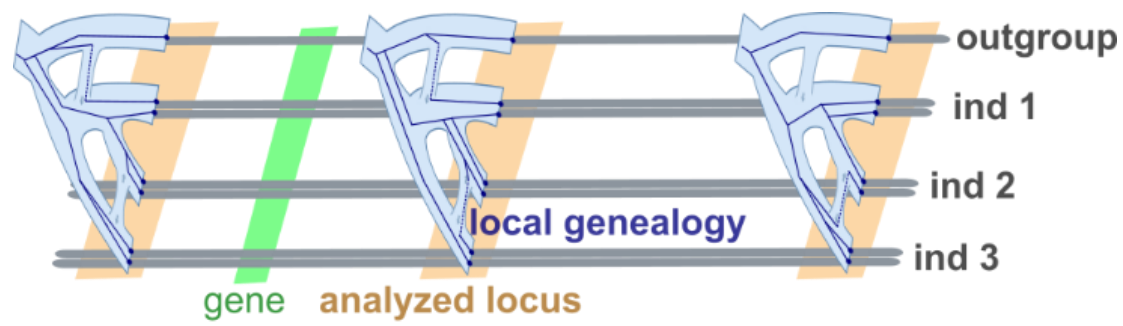
\includegraphics[width=0.8\textwidth]
{multiple_loci_across_sequence}
\captionsetup{width=.8\textwidth}
\caption{\gp uses independant loci, chosen to be far away from genes and from each other to reduce the influence of selection and accomodate the assumption of independence. A local genealogy is represented over each locus and embedded in the population phylogeny.}
\label{fig:multiple_loci_across_sequence}
\end{figure}


\subsection{The Model Selection Problem}

The model selection problem takes sequence data and a series of models $\M_1,... \M_n$, which differ in their structural components, and aims to find the one which best fits the data set, i.e. select the model $\M_i$ with maximal $P(X|\M_i)$. Typically only the structural assumptions of the models are compared ($\Tr$ and $B$), and not specific parameter values ($\T$).


\begin{figure}[h]
\centering
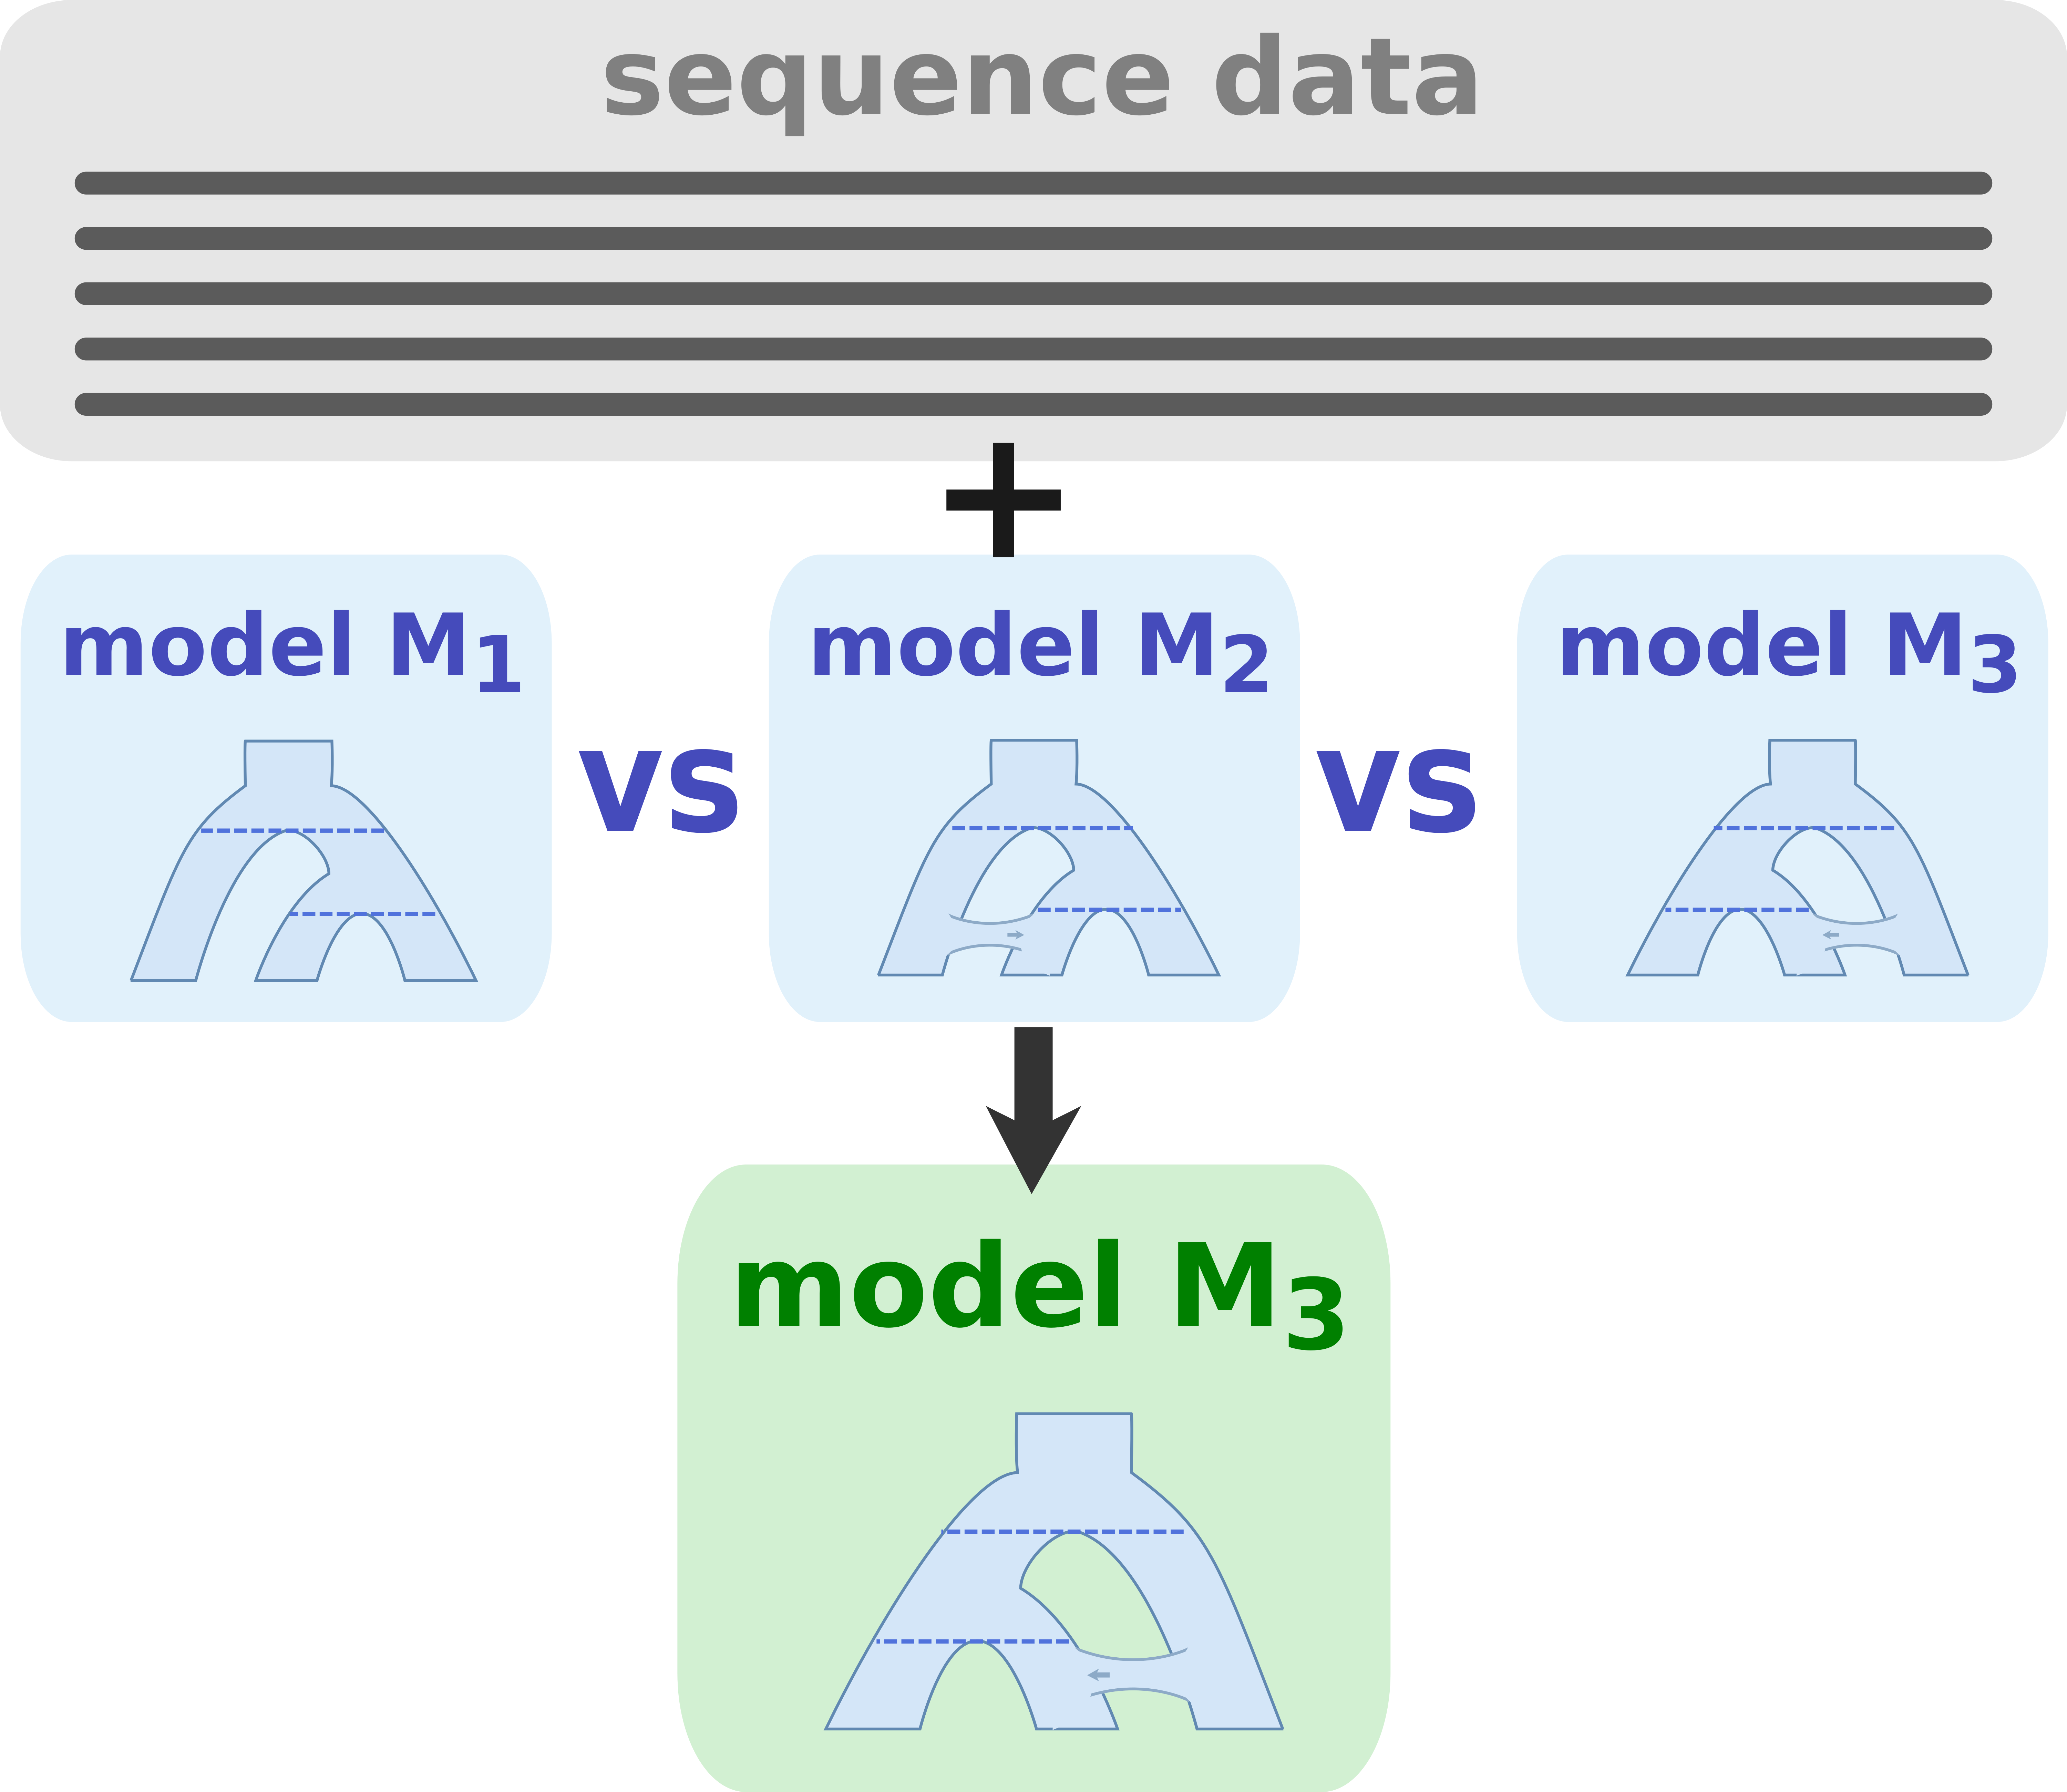
\includegraphics[width=0.6\textwidth]
{by_ilan/probgen_3_model_selection}
\captionsetup{width=.8\textwidth}
\caption{An example problem of selecting between three models with different topological structures. Mdoel $\M_1$ has three leaf populations and no migration. Model $\M_2$ has the same phylogeny as $\M_1$ but with an additional migration band. In model $\M_3$ the relationship between leaves is different. 
%
Given aligned sequence data and a set of structural hypotheses, we wish to choose which structural model best fits the data.}
\label{fig:model_A__OR__model_b}
\end{figure}


%
In this study, building upon the \gp demography inference method and MCMC sampler, we develop the theoretical framework for a robust model-selection scheme, and implement a method for comparing models and their fit to the data, this without analytically calculating $P(X|\M_i)$.

\section{Methods}


\subsection{Estimating data likelihood via importance sampling}

Model fit is best captured by the marginal data likelihood, $P(\X|\M)$, whose computation involves integration over the space of unknown parameter values and genealogical relationships,
denoted jointly by $\GT$.
%
This high-dimensional integral may be approximated via importance sampling using a collection of instances $\{\GT^{(i)}\}$ sampled via MCMC conditioned on $\X$ and $\M$.
%
The approximation is established by expressing the inverse of the likelihood as an expected value under the posterior distribution of $\GT$ given $\M$ and $\X$:
%
%
\begin{small}
\begin{align}
%\frac{1}{\hbf(\M|\X)} ~~~ \triangleq~~
\frac{1}{P(\X|\M)} ~~~
&=~~ \frac{\int P(\GT|\M)d\GT}{P(\X|\M)} \notag \\ %
&=~~ \int \frac{P(\GT|\M)}{P(\X|\M)} \frac{P(\X,\GT|\M)}{P(\X,\GT|\M)}  d\GT \notag \\ %
&=~~ \int \frac{P(\GT,\X |\M)}{P(\X|\M)} ~\bigg/ \frac{P(\X,\GT|\M)}{P(\GT|\M)}  d\GT \notag \\ %
&=~~ \int \frac{P(\GT|\M,\X)}{P(\X|\M,\GT)} d\GT \notag \\ %
&=~~ \int \frac{1}{P(\X|\G)}P(\GT|\M,\X) d\GT  \notag \\ %
&=~~ \E_{\GT|\M,\X } \left[\frac{1}{P(\X|\G)}\right] \notag\\  %~.\label{eq:is_harmonic}\\
%\notag \\ %
%\frac{1}{P(\X|\M)}
&\approx~~ \frac{1}{N} \sum_{i=1}^{N}\frac{1}{P(\X|\G^{(i)})} ~. \label{eq:harmonic}
\end{align}
\end{small}

This {\em harmonic mean estimator} is straightforward and can be applied in a very general setting, but its practical use is often limited due to very high variance
of the inverse likelihood, $1/P(\X|\G)$.
%
This high variance means that only models with very different levels of fit may be compared reliably via harmonic mean estimators of $P(\X|\M)$.
%
The main objective of the approach we propose next is to correlate the sensitivity of model comparison with the level of similarity between the models being compared.
%

\subsection{Relative Bayes factors}
\label{Relative Bayes factors}

We propose here an alternative way to evaluate the fit of model $\M$ by estimating its likelihood relative to some
reference model $\Mref$. 
%
As before, assume a collection $\{\GT^{(i)}\}$ sampled via MCMC according to an approximate posterior probability distribution $P(\GT|\M,\X)$.
%
We wish to use these MCMC samples to estimate the {\em Bayes factor of $\M$ relative to $\Mref$}, defined as the ratio $P(\X|\M) / P(\X|\Mref)$.
%
The Bayes factor can be estimated by running an additional MCMC for $\Mref$ and taking the ratio of the two harmonc-mean estimates for $P(\X|\M)$ and $P(\X|\Mref)$.
%
However, in some cases the relative Bayes factor may be estimated directly from $\{\GT^{(i)}\}$ without the need for an additional MCMC for $\Mref$.
%
This is done by connecting the models $\M$ and $\Mref$ via a conditional distribution over the the hidden variables of $\M$, $\Pref(\GT|\Mref)$,
which satisfies the following two requirements:
%
%
\begin{small}
\begin{align}
&P(\X|\Mref) ~~=~~ \int  \Pref(\GT|\Mref)\ P(\X|\G)\ d\GT \label{eq:pref_integral}\\
&P(\GT|\M,\X)=0 ~~\Rightarrow~~ \Pref(\GT|\Mref)=0 \label{eq:pref_support}
\end{align}
\end{small}
%
%


The \emph{model pairing conditional distribution}, $\Pref(\GT|\Mref)$, plays a key role in our estimator for the relative Bayes factor.
%
The special notation $\Pref$ indicates that this probability function is not naturally defined by either
$\M$ or $\Mref$, and there will typically be some degree of freedom associated with its specification.
%
Given a model-pairing conditional distribution, the relative Bayes factor  may be expressed as an expected value under the posterior distribution of $\GT$ given $\M$ and $\X$,
implying the following approximation:
%
%
\begin{small}
\begin{align}
\frac{1}{\rbf(\M:\Mref|\X)} ~~~ \triangleq ~~ \frac{P(\X|\Mref)}{P(\X|\M)}
&=~~ \frac{\int  \Pref(\GT|\Mref)\ P(\X|\G)\ d\GT}{P(\X|\M)} \label{eq:pref1} \\ %
&=~~ \int \frac{\Pref(\GT|\Mref)\ P(\X|\G) }{P(\X|\M)} \ \frac{P(\GT|\M, \X)}{P(\GT|\M, \X)}  d\GT \label{eq:pref2} \\ %
&=~~ \int \frac{\Pref(\GT|\Mref)\ P(\X|\G)\ }{P(\X,\GT|\M)} P(\GT|\M, \X)  d\GT \notag \\ %
&=~~ \int \frac{\Pref(\GT|\Mref) }{P(\GT|\M)} P(\GT|\M, \X)  d\GT  \label{eq:data_cancel}\\ %
&=~~ \E_{\GT|\M,X } \left[\frac{\Pref(\GT|\Mref) }{P(\GT|\M)}\right]~.\notag \\
&\approx~~ \frac{1}{N} \sum_{i=1}^{N}\frac{\Pref(\GT^{(i)}|\Mref) }{P(\GT^{(i)}|\M)} ~.\label{eq:rbf}
\end{align}
\end{small}
%
%

Note that the condition of Equation \ref{eq:pref_integral} implies the equality in Equation \ref{eq:pref1},
and the condition of Equation \ref{eq:pref_support} guarantees no division-by-zero in Equation \ref{eq:pref2}.
%
Interestingly, the contribution of the data to the likelihood cancels out in Equation \ref{eq:data_cancel} (because it is equal in both models).
%
Thus the ratio used for estimation, ${\Pref(\GT|\Mref) }/{P(\GT|\M)}$, is not a direct function of the data ($\X$),
and the data affects the estimate only through its influence the sampled instances $\{\GT^{(i)}\}$.
%
We refer to the ratio in Equation \ref{eq:pref1} as the {\em relative Bayes factor (RBF) ratio}, and employ it as a model selection criteria by comparing RBFs of competing hypothesis models, calculated using the same reference model - 
\[ \frac{1}{\rbf(\M_i:\Mref|\X)} >  \frac{1}{\rbf(\M_j:\Mref|\X)} \Rightarrow P(\X|\M_j) >  P(\X|\M_i)\]


Importantly, the variance of the RBF depends on the definition of the model-pairing conditional, $\Pref$, and it will typically decrease as $\M$ and $\Mref$ become more similar.
%
For instance, in the trivial case where $\Mref=M$, we can define $\Pref(\GT|\Mref)=P(\GT|\M)$ and the RBF ratio becomes 1 for all instances $\{\GT^{(i)}\}$.
%
This is the key advantage of direct estimation of the Bayes factor, when compared to estimation via harmonic mean, and realizing this advantage requires construction of an effective model-pairing conditional distribution for $\M$ and $\Mref$.
%
The following sections present specific constructions for $\Pref$ in a series of cases.

\subsection{The null reference model $\M_0$}
\label{The null reference model}
We start by considering a simple case where $\M$ is a demographic model with no migration bands and $\Mref$ is the simplest possible model with a single population $p_0$ of constant size $\theta_0$.
%
We refer to this simple one-parameter model as the {\em null reference model} $\M_0$ (figure \ref{fig:null_reference_model_no_migration}).
%
\begin{figure}[h]
\centering
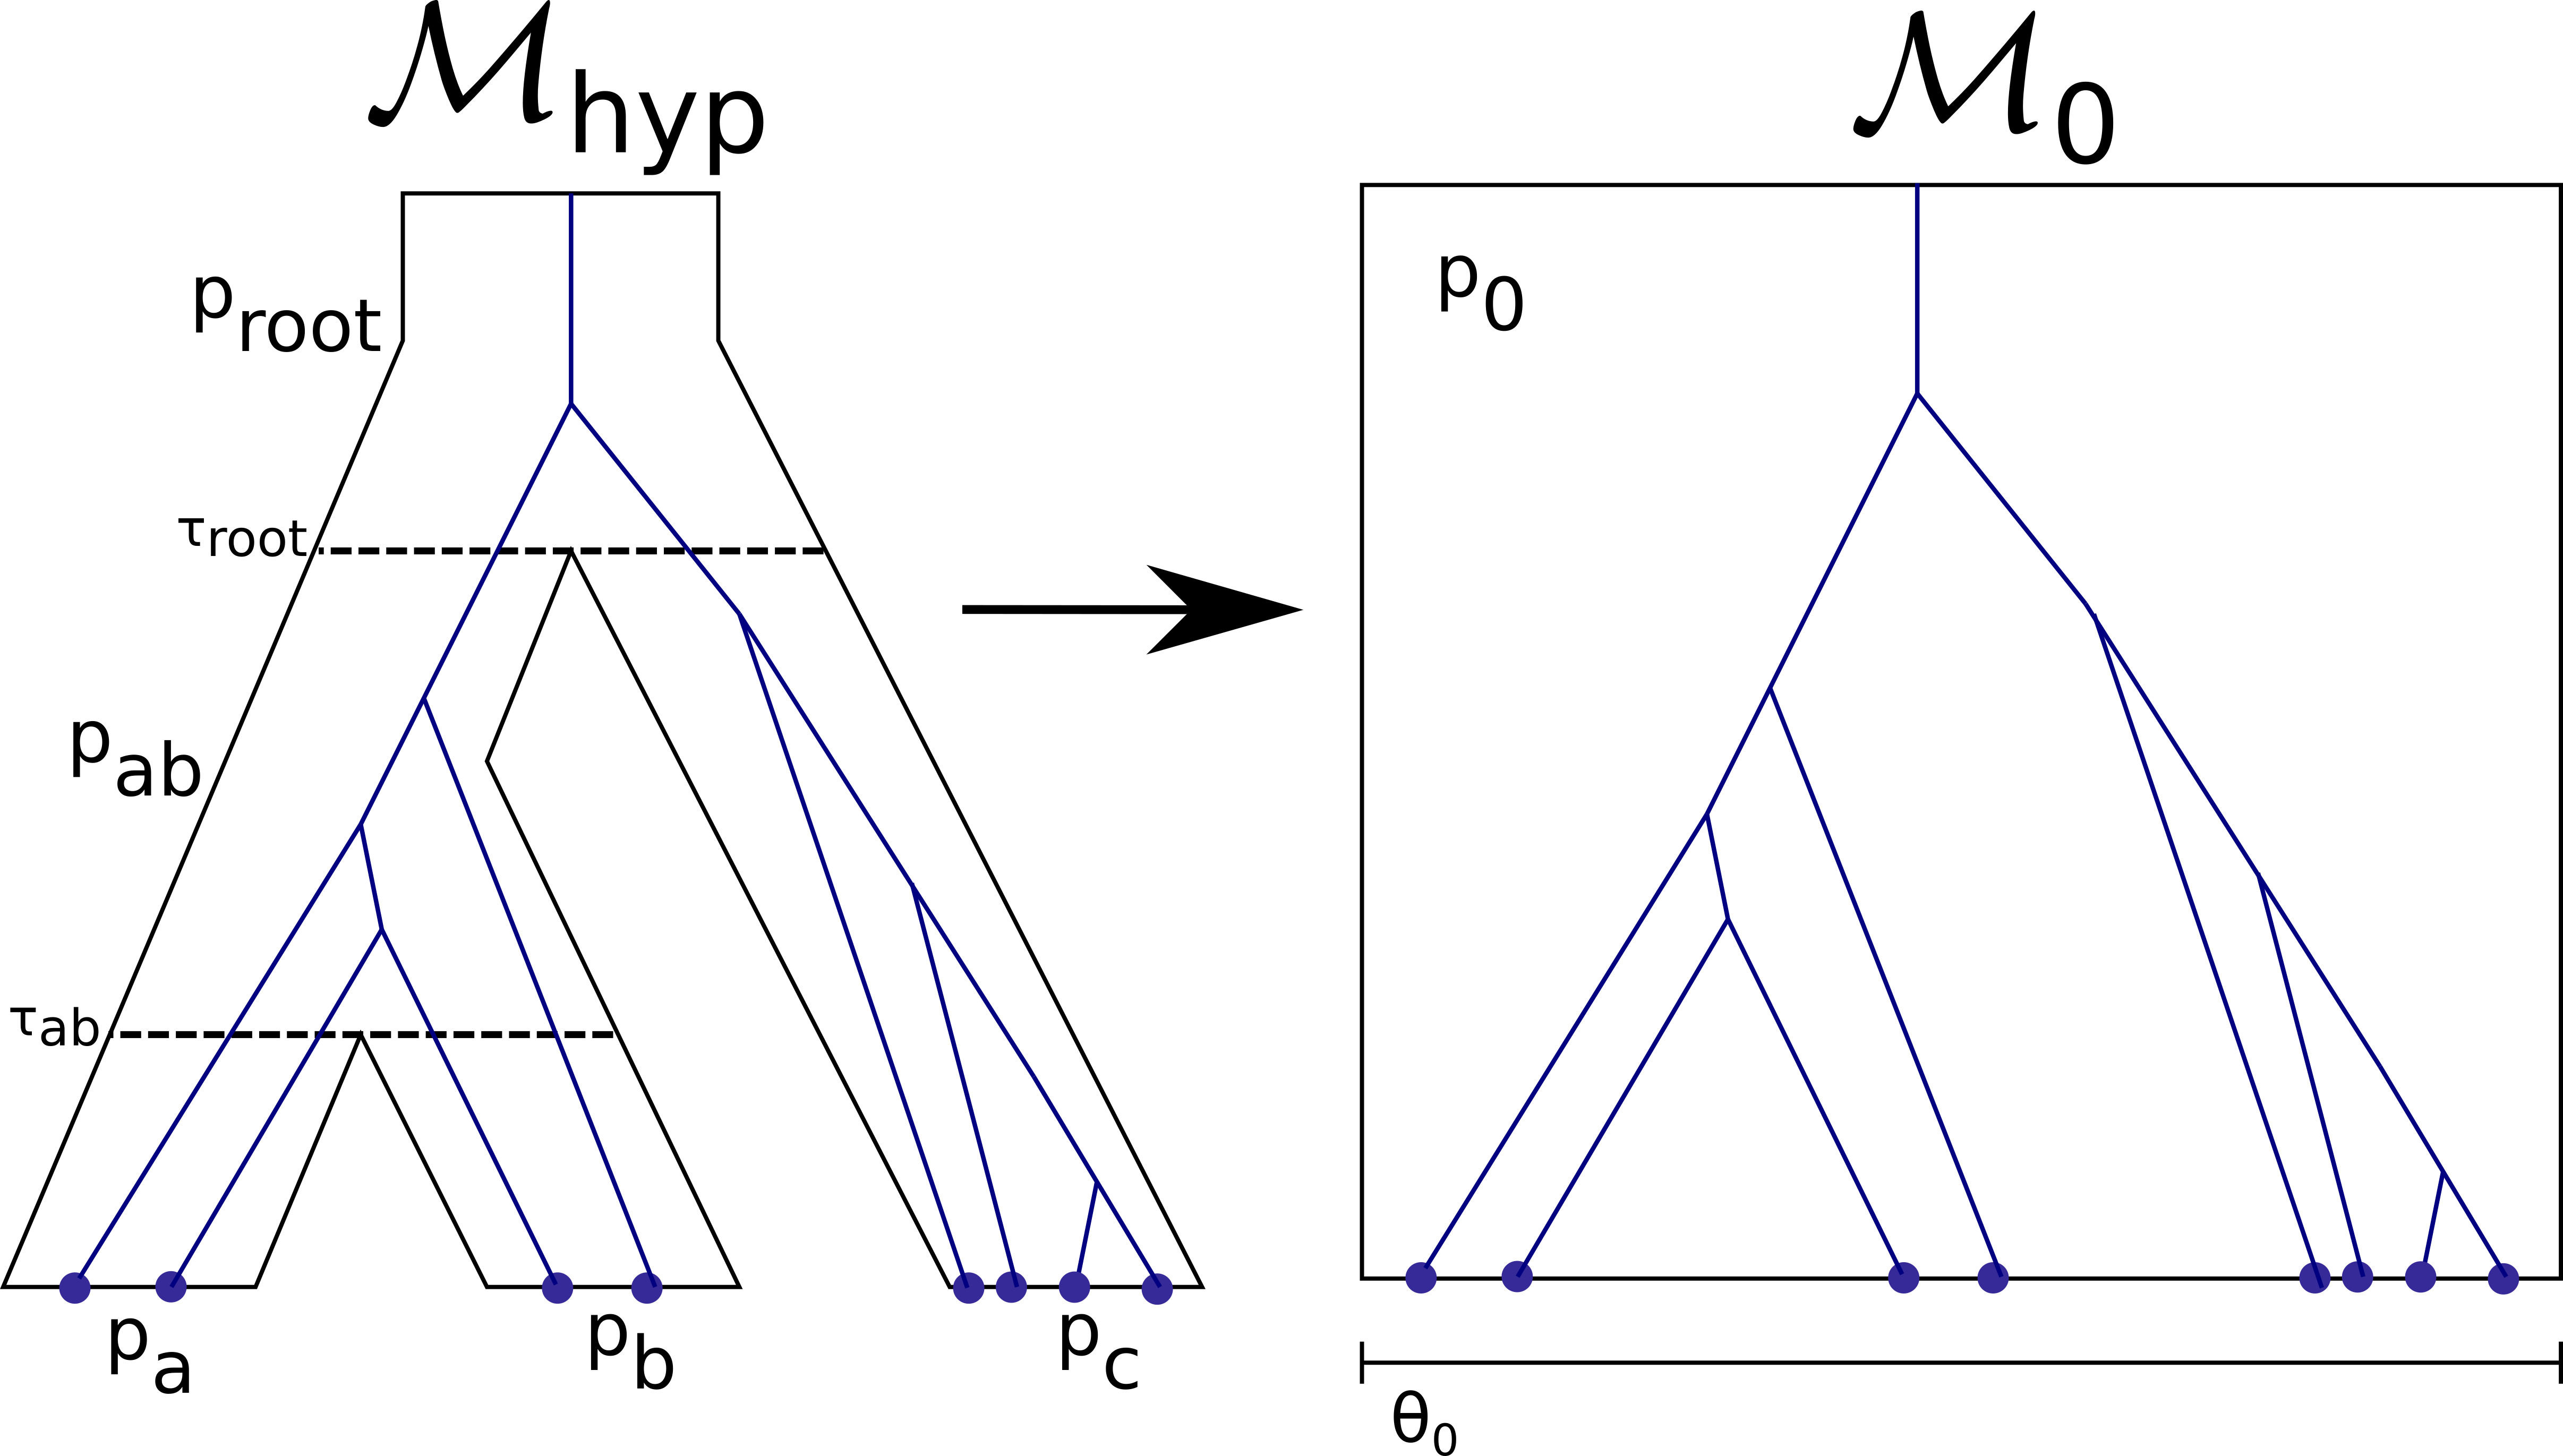
\includegraphics[width=0.8\textwidth]
{null_reference_model_no_migration}
\captionsetup{width=.8\textwidth}
\caption{A mapping from hypothesis model $\M_{hyp}$ onto the null reference model $\M_0$. Population sizes $\{\theta_{p_a}, \theta_{p_b}, \theta_{p_c}, \theta_{p_{ab}}\}$ are mapped according to their prior probability in $\M_{hyp}$. These have no effect on the reference model structure. Divergence times $\{\tau_{ab}, \tau_{root}\}$ are mapped onto a uniform distribution with upper bound calculated as described in appendix \ref{ap:cond_nomig}. The  hypothesis parameter $\theta_{root}$ is mapped onto the free parameter of the reference model $\theta_0$ to minimize RBF variance.}
\label{fig:null_reference_model_no_migration}
\end{figure}
%
The first step of constructing a model-pairing conditional for the two models is to identify a mapping $F$ from the space
of hidden variables in $\M$ to the space of hidden variables in $\M_0$.
%
In our case, denote by $\Gref$ and $\Tref$ the hidden variables of $\M_0$.
%
Because both $\M$ and $\M_0$ have no migration bands, then we may assume that the genealogical information used
by both models is the same, implying a natural one-to-one mapping between $\G$ and $\Gref$ (the implications of migration are discussed in the next section).
%
A mapping between $\T=(\taus,\thetas)$ and $\Tref=(\theta_0)$ can be defined by selecting one of the population size parameters in $\T$
to be associated with $\theta_0$. This can be the size of the root population, $\troot$, or any other population
that we expect to best represent the single population in $\M_0$.
%
The model pairing conditional is obtained by applying this mapping and extending it to the unmapped hidden variables, $~ \Z=(\taus,\thetas\setminus \{\troot\})$, with the use of a conditional distribution, $\Pref(\Z|\GT\setminus\Z)$:
%
%
\begin{small}
\begin{equation}
 \Pref(\GT|\M_0)  ~~=~~
 P(\theta_0=\troot|\M_0)\ P(\Gref=\G|\M_0,\theta_0=\troot)\ \Pref(\Z|\G,\troot)   ~ .\label{eq:pref_null}
\end{equation}
\end{small}
%
%
The model-pairing condition of Equation \ref{eq:pref_integral} is thus established, regardless of how $\Pref(\Z|\G,\troot)$ is defined:
%
%
\begin{small}
\begin{align}
P(\X|\M_0)
&=~~ \int P(\Tref|\M_0)\ P(\Gref|\M_0,\Tref)\ P(\X|\Gref)\   d\Gref d\Tref  \notag \\ %
&=~~ \int P(\theta_0=\troot|\M_0)\ P(\Gref=\G|\M_0,\theta_0=\troot)\ P(\X|\G)\  d\G d\troot \notag \\ 
&=~~ \int P(\theta_0=\troot|\M_0)\ P(\Gref=\G|\M_0,\theta_0=\troot)\ P(\X|\G)\
\left( \int \Pref(\Z|\G,\troot)\ d\Z \right) d\G d\troot \notag \\ 
%
&=~~ \int P(\theta_0=\troot|\M_0)\ P`(\Gref=\G|\M_0,\theta_0=\troot)\ \Pref(\Z|\G,\troot)\ P(\X|\G)\ d\GT \notag \\ 
&=~~ \int \Pref(\GT|\M_0)\ P(\X|\G)\ d\GT ~. \label{eq:likelihood_null} %
\end{align}
\end{small}

We are left to construct $\Pref(\Z|\G,\troot)$ so that it ensures the model-pairing condition of Equation \ref{eq:pref_support},
and we wish to use the remaining degree of freedom to minimize the variance of the RBF ratio.
%
Equation \ref{eq:pref_support} is guaranteed by constricting $\Pref(\Z|\G,\troot)$ to have zero values whenever $P(\G,\troot,\Z|\M,\X)=0$.
%
Among the unmapped variables $\Z=(\taus,\thetas\setminus \{\troot\})$, the population size parameters $\thetas\setminus \{\troot\}$ do not 
pose any restrictions on the mapped variables $\G,\troot$. This means that Equations \ref{eq:pref_support} is guaranteed regardless of how their marginal distribution is defined.
%
We thus define their conditional probability distribution according to their prior probability in $\M$, to cancel out terms in the RBF ratio and potentially reduce its variance.
%
\begin{small}
\begin{align}
\frac{\Pref(\GT|\M_0) }{P(\GT|\M)}
&=~~ \frac{ P(\theta_0=\troot|\M_0) ~ P(\G|\M_0,\theta_0=\troot) ~ \Pref(\Z|\G,\troot)} {P(\GT|\M)} \notag \\
&=~~ \frac{ P(\G|\M_0,\theta_0=\troot) }{ P(\G|\M,\T)}~ 
     \frac{ P(\theta_0=\troot|\M_0) \prod_{p\neq \troot}\Pref(\theta_p|\G,\troot) }{P(\troot|\M)\prod_{p\neq \troot}P(\theta_p|\M)}~
     \frac{ \Pref(\taus|\G,\thetas)}{P(\taus|\M)} \notag \\
&=~~ \frac{ P(\G|\M_0,\theta_0=\troot) }{ P(\G|\M,\T)}~ 
     \frac{ P(\theta_0=\troot|\M_0)}{P(\troot|\M)}\
     \frac{ \Pref(\taus|\G,\thetas)}{P(\taus|\M)} ~. \label{eq:rbf_null}
\end{align}
\end{small}

Note that if we assume that $\M$ and $\M_0$ use the same prior distribution over $\theta_{root}$ and $\theta_0$ (resp.),
then the middle term in Equation \ref{eq:rbf_null} also cancels out.
%
We cannot similarly define $\Pref(\taus|\G,\thetas)=P(\taus|\M)$, because this may lead to conflicts between divergence times and coalescence times in $\G$, which result in violation of
the model-pairing condition of Equation \ref{eq:pref_support}.
%
Such conflicts occur when a divergence time $\tau_p$ is deeper than the most recent common ancestor
in $\G$ of two individuals that are each a descendant of a different daughter population of population $p$.
%
% Because such a conflict implies that $P(\GT|\M) = 0$, we must also guarantee that $\Pref(\{\tau_p\}|\G)=0$.
%
Thus, the final step of constructing $\Pref(\GT|\Mref)$ is to construct $\Pref(\taus|\G,\thetas)=\Pref(\taus|\G)$ to have zero values whenever $P(\G|\M,\taus,\thetas)=0$.
%
This guarantee is achieved by computing for each $\tau_p$ an upper bound based on the coalescent events in $\G$
and defining $\Pref(\taus|\G)$ as a product of uniform distributions in the feasible ranges of $\taus$
%
(see  Appendix \ref{ap:cond_nomig} for complete derivation and proof).


\subsection{Models with gene flow}

Assume now that the reference model is still the null model, $\M_0$, but the model of interest, $\M$, has a non-empty
set of migration bands, $B$, associated with migration rate parameters, $\migs=\{m_b:b\in B\}$.
%
Migrations complicate the mapping between $\M$ and $\M_0$ because the genealogies in $\M$ hold information
about migration events, but the genealogies in $\M_0$ do not.
%
For a sequence of local genealogies $\G$ in $\M$, denote by $\Gc$ the coalescent trees implied by $\G$
and denote by $\Gm$ the information on migration events in $\G$ (locus, timing of event, branch in $\Gc$, source and target populations).
%
%Because the genealogies $\Gref$ in $\M_0$ have no migration events, then t
%There is a natural mapping between $\Gc$ (of $\M$) and $\Gref$ (of $\M_0$) and $P(\X|\Gref) = P(\X|\Gc)$.
Thus, a mapping between the hidden variables of $\M$ ($\Gc,\Gm,\T$) and the hidden variables of $\M_0$ ($\Gref,\theta_0$) can be defined by
mapping $\Gc$ to $\Gref$ and mapping some $\troot\in\T$ to $\theta_0$.
%
Consequently, the set of unmapped hidden variables is $\Z~=~ (\Gm,\taus,\migs,\thetas\setminus\{\troot\})$.
%
This implies a slight modification of the model-pairing conditional specified in Equation \ref{eq:pref_null}:
%
%
\begin{small}
\begin{align}
 \Pref(\GT|\M_0)
 &=~~ 
 %\Pref(\Gc,\troot,\Z|\M_0) ~~=~~
 P(\theta_0=\troot|\M_0)\  P(\Gref=\Gc|\M_0,\theta_0=\troot)\ \Pref(\Z|\Gc,\troot)  ~ .\label{eq:pref_mig}
\end{align}
\end{small}

The model-pairing condition of Equation \ref{eq:pref_integral} can be confirmed  by following a sequence of equalities similar to the ones we derived for 
the scenario without migration (see Equation \ref{eq:likelihood_null}).
%
We are thus left to specify the conditional distribution $\Pref(\Z|\Gc,\troot)$ to ensure that all $\GT$ for which $P(\Gc,\troot,\Z|\M,\X)=0$
also satisfy $\Pref(\Z|\Gc,\troot)=0$.
%
Since the genealogy trees $\Gc$ do not restrict the population size and migration rate parameters, we may define
the conditional probability for these parameters based on their prior probability under $\M$, so that their terms cancel out in the RBF ratio:
%
%
\begin{small}
\begin{align}
\frac{\Pref(\GT|\M_0) }{P(\GT|\M)}
&=~~ \frac{ P(\theta_0=\troot|\M_0) ~  P(\Gref=\Gc|\M_0,\theta_0=\troot) ~ \Pref(\Z|\Gc,\troot) } {P(\GT|\M)} \notag \\
&=~~ \frac{ P(\Gc|\M_0,\theta_0=\troot) }{ P(\Gc,\Gm|\M,\T)}~ 
     \frac{ P(\theta_0=\troot|\M_0) \prod_{p\neq root}\Pref(\theta_p|\Gc,\troot)~\prod_{b}\Pref(m_b|\Gc,\troot) }{P(\troot|\M)\prod_{p\neq\troot}P(\theta_p|\M)~\prod_{b}P(m_b|\M)}~
     \frac{ \Pref(\taus,\Gm|\Gc)}{P(\taus|\M)} \notag \\
&=~~ \frac{ P(\Gc|\M_0,\theta_0=\troot) }{ P(\Gc,\Gm|\M,\T)}~ 
     \frac{ P(\theta_0=\troot|\M_0)}{P(\troot|\M)}\
     \frac{ \Pref(\taus,\Gm|\Gc)}{P(\taus|\M)} ~. \label{eq:rbf_mig}
\end{align}
\end{small}

As in the case without migration, we are left to define the conditional probability distribution over the restricting hidden variables, which are in this case the divergence times
$\taus$ and the migration events $\Gm$.
%
The complex dependence between divergence times and migration events makes this particularly challenging.
%
For instance, a migration event between populations $p_1$ and $p_2$ at time $t$ implies that the divergence times of all populations ancestral to $p_1$ and $p_2$ is at least $t$,
%
but at the same time this migration event may also relax the upper bound of these divergence times.
%
Thus, bounds on divergence times cannot be determined solely based on $\Gc$, and the conditional $\Pref(\taus,\Gm|\Gc)$ cannot be factored into a product of
two separate probability distributions for $\taus$ and $\Gm$.
%
In Appendix \ref{ap:cond_mig} we present a specification for the joint conditional distribution $\Pref(\taus,\Gm|\Gc)$,
which addresses this complex dependence and ensures that $\Pref(\taus,\Gm|\Gc)=0$ whenever $P(\taus,\Gm,\Gc|\M)=0$.
%%
This construction results in additional terms canceling out with terms in  the genealogy likelihood
$P(\Gc,\Gm|\M,\T)$, to further reduce the variance of the RBF ratio.


\subsection{The comb reference model} \label{The comb reference model} 


The null model has the unique advantage of being a valid reference for the comparison of any two models.
This advantage, however, comes at the cost of collapsing all population structure.
%
In many cases we know the population designation of the sampled individuals, and model uncertainty is restricted to the relationships between the sampled populations.
%
To capture this simple structure we use a population phylogeny with a single ancestral population splitting simultaneously into all sampled populations.
We refer to such reference models as {\em comb} models and denote them by $\Mcomb$,  due to the comb-like structure of the population phylogeny.
%
A comb model is defined by: (1) a set of sampled (leaf) populations, $L$; (2) an ancestral population, $comb$; and (3) a set of migration bands $B_L$ between populations in $L$.
%
The resulting demographic model, $\Mcomb(L,B_L)$, has $|B_L|+|L|+2$ parameters: $\Tref ~=~ (\tacomb, \widetilde{\thetas},\widetilde{\migs})$,
where $\widetilde{\thetas}=\{\theta_p:p\in L\cup \{comb\}\}$ and $\widetilde{\migs} = \{m_b:b\in B_L\}$.
%

\begin{figure}[h]
\centering
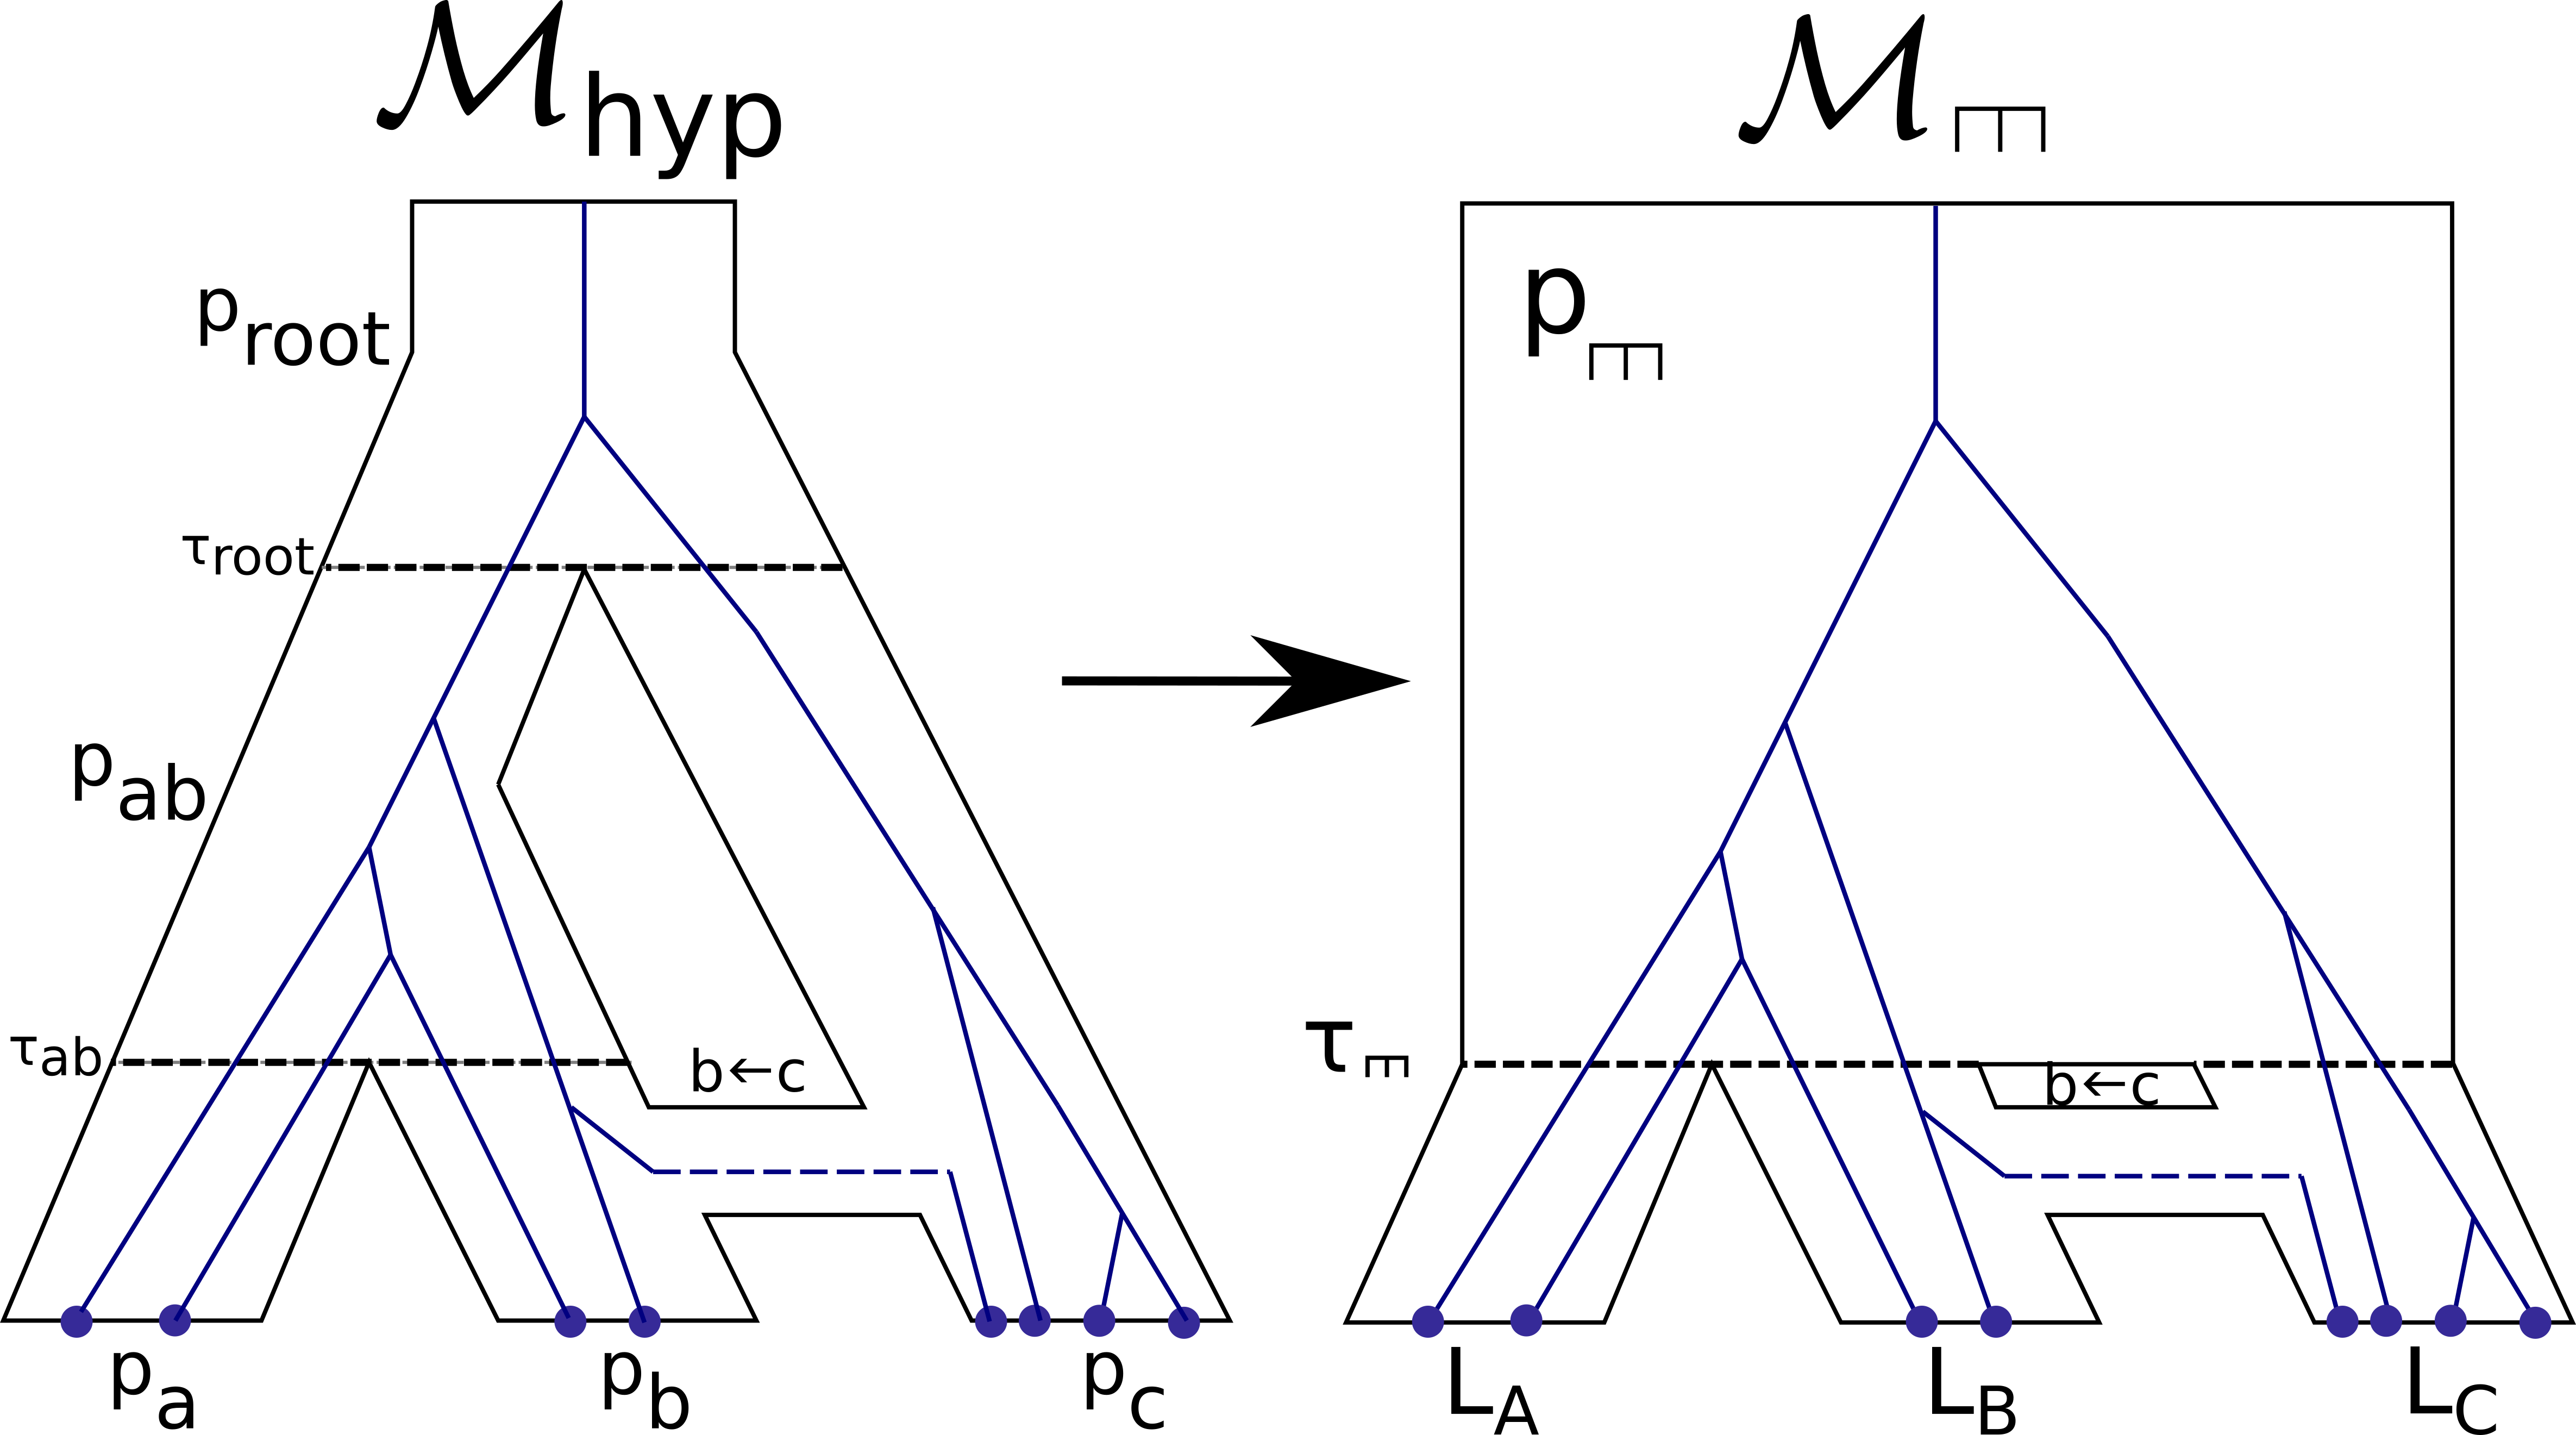
\includegraphics[width=0.8\textwidth]
{comb_model_with_migration_single_genealogy}
\captionsetup{width=.8\textwidth}
\caption{A mapping from a hypothesis model with a migration band $\M_{hyp}$ onto the null reference model $\M_0$. Population sizes $\{\theta_{p_a}, \theta_{p_b}, \theta_{p_c}, \theta_{p_{ab}}\}$ and migration rate $m_{B->C}$ are mapped according to their prior probability in $\M_{hyp}$. These have no effect on the reference model structure. Divergence times $\{\tau_{ab}, \tau_{root}\}$ are mapped onto a uniform distribution with upper and lower bounds calculated as described in appendix \ref{ap:cond_mig}. The remaining hypothesis parameter $\theta_{root}$ is mapped onto the free parameter of the reference model $\theta_{p_0}$ so as to minimize the RBF ratio.
}
\label{fig:comb_model_with_migration_single_genealogy}
\end{figure}


%
Consider a demographic model, $\M(\Tr,B)$, and its corresponding comb model, $\Mcomb(L,B_L)$, defined by $L=leaves(\Tr)$ and $B_L=B \cap (L \times L)$.
%
For brevity, we refer to $\Mcomb(L,B_L)$ simply as $\Mcomb$.
%
The model-pairing conditional distribution for $\M$ and $\Mcomb$ is constructed by first defining a mapping between the hidden variables of $\M$ ($\GT$) and the hidden variables of $\Mcomb$ ($\Gref\Tref$).
%
This mapping is derived from the requirement that below the comb divergence time ($\tacomb$) the comb model is identical to $\M$ and above it $\Mcomb$ is identical to the null model $\M_0$.
%
We thus set $\tacomb=\tmin\eqdef\min(\taus)$, to guarantee that all population divergence events in $\M$ map to the comb population in $\Mcomb$.
%
The migration rates of bands in $\B \cap (L \times L)$ and effective sizes of populations in $L$ are mapped into their counterparts in $\Tref$,
%
and following the mapping for the null model, a single ancestral population size parameter ($\troot$) is chosen to be mapped into $\thcomb$.
%
We denote the set of mapped migration rate and population size parameters of $\M$ collectively as $\Tcomb$.
%
Mapping between genealogies is obtained by {removing from $\G$ all migration events above time $\tmin$}.
The resulting collection of local genealogies are denoted by $\Gcomb$ and are directly mapped to $\Gref$.
%
The remaining unmapped hidden variables ($\Z$) of $\M$ consist of the following components:
\begin{enumerate}
 \item Unmapped population size parameters: $\{\theta_p : p\notin L\cup \{root\}\ \}$.
 \item Unmapped migration rate parameters:  $\{m_b: b\notin L \times L \}$.
 \item The identity of the ancestral population in $\Tr$ with minimum divergence time: $minAncPop=\argmin(\taus)$. 
   Note that this population may be \emph{any ancestral population with two leaf daughters}, and its identity is lost when mapping $\taus$ into $\tacomb$.
 \item The divergence times of all other populations: $\{\tau_p:p\neq minAncPop\}$.
 \item Information on all migration events in $\G$ above time $\tacomb$, which we denote by $\G_{m|>\tmin}$.
\end{enumerate}


A model-pairing conditional distribution for $\M$ and $\Mcomb$ is thus established by applying the mapping described above and
specifying a conditional distribution over the unmapped parameters, $\Pref(\Z|\Gcomb,\Tcomb,\tmin)$. The proof of the condition in Equation \ref{eq:pref_integral} is given below:
%
%
\begin{small}
\begin{align}
 \Pref(\GT|\Mcomb)
 &=
 P(\Tref=(\Tcomb,\tmin)|\Mcomb)\ P(\Gref=\Gcomb|\Mcomb,\Tcomb,\tmin)\ \Pref(\Z|\Gcomb,\Tcomb,\tmin)  ~ .\label{eq:pref_comb}\\
%\notag \\
%\end{align}
%\end{small}
%
%
%\begin{small}
%\begin{align}
P(\X|\Mcomb)
&= \int P(\Tref|\Mcomb)\ P(\Gref|\Mcomb,\Tref)\ P(\X|\Gref)\   d\Gref\Tref  \notag \\ %
&= \int P(\Tref=(\Tcomb,\tmin)|\Mcomb)\ P(\Gref=\Gcomb|\Mcomb,\Tcomb,\tmin)\ P(\X|\Gcomb)\  ~ d\Gcomb\Tcomb\tmin \notag \\ 
&= \int P(\Tref=(\Tcomb,\tmin)|\Mcomb)\ P(\Gref=\Gcomb|\Mcomb,\Tcomb,\tmin)\ P(\X|\Gcomb) \left( \int \Pref(\Z|\Gcomb,\Tcomb,\tmin) d\Z \right) d\Gcomb\Tcomb\tmin \notag \\ 
&= \int P(\Tref=(\Tcomb,\tmin)|\Mcomb)\ P(\Gref=\Gcomb|\Mcomb,\Tcomb,\tmin)\ \Pref(\Z|\Gcomb,\Tcomb,\tmin)\ P(\X|\G)\   d\GT \notag \\ 
&= \int \Pref(\GT|\M_0)\ P(\X|\G)\ d\GT ~. \label{eq:likelihood_comb} %\\
%\notag \\
\end{align}
\end{small}

The conditional distribution $\Pref(\Z|\Gcomb,\Tcomb,\tmin)$ is defined similar to its specification in the null model.
%
The unmapped population size and migration rate parameters are distributed according to their prior probability under $\M$ to eliminate terms in the RBF ratio.
%
The identity of the minimal ancestral population, $minAncPop$, is distributed uniformly among all ancestral populations in $\Tr$ with two leaf daughters.
%
We denote the number of such populations in $\Tr$ by $\kappa(\Tr)$.
%
The only unmapped variables restricted by $\Gcomb$ and $\tmin$ are the unmapped divergence times and migration events above time $\tmin$. Their conditional distribution,
$\Pref(\taus\setminus\{\tmin\},\G_{m|>\tmin}|\Gc)$, is defined using the process described for the null model (see Appendices \ref{ap:cond_nomig} and \ref{ap:cond_mig}).
%
This specification thus guarantees the condition of Equation \ref{eq:pref_support}, as in the case of the null reference model.
%
The resulting RBF ratio is expressed as follows:
%
%
\begin{small}
\begin{align}
\frac{\Pref(\GT|\Mcomb) }{P(\GT|\M)}
&= \frac{ P(\Tref=(\Tcomb,\tmin)|\Mcomb) ~ P(\Gref=\Gcomb|\Mcomb,\Tcomb,\tmin) ~ \Pref(\Z|\Gcomb,\Tcomb,\tmin) } {P(\GT|\M)} \notag \\
&= \frac{ P(\Gref=\Gcomb|\Mcomb,\Tcomb,\tmin) }{ P(\G|\M,\T)}~ 
   \frac{ P(\Tref=(\Tcomb,\tmin)|\Mcomb) }{ P(\Tcomb|\M) }~
   \frac{ \frac{1}{\kappa(\Tr)}\Pref(\taus\setminus\{\tmin\},\G_{m|>\tmin}|\Gc)}{P(\taus|\M)} ~. \label{eq:rbf_comb}
\end{align}
\end{small}


As in the case of the null reference model, the above RBF ratio has several terms canceling out. First, the conditional probabilities of the unmapped population size and
migration rate parameters cancel out with their priors under $\M$. Second, if we assume identical priors in both models for the mapped parameters,
then these cancel out as well in the second term of Equation \ref{eq:rbf_comb}.
Terms in the genealogy likelihood contributed by migration events above time $\tmin$ also cancel out in the ratio (see Appendix \ref{ap:cond_mig}).
Finally, the contribution of all events below time $\tmin$ (coalescence and migration) also cancel out.
If we denote the portion of $\G$ below time $\tmin$ by $\G_{<\tmin}$, and the portion above it by $\G_{>\tmin}$, then the contribution of $\G_{<\tmin}$ 
to the first term of the RBF ratio cancels out as follows:
%
%
\begin{small}
\begin{align}
\frac{ P(\Gcomb|\Mcomb,\Tcomb,\tmin) }{ P(\G|\M,\T)}
&=~~ \frac{ {P(\Gcomb}_{<\tmin}|\Mcomb,\Tcomb,\tmin) P({\Gcomb}_{>\tmin}|\Mcomb,\Tcomb,\tmin) }{ P(\G_{<\tmin}|\M,\T) P(\G_{>\tmin}|\M,\T)}   \notag \\
&=~~ \frac{ {P(\G}_{<\tmin}|\Mcomb,\Tcomb,~\tacomb=\tmin)}{ P(\G_{<\tmin}|\M,\Tcomb,~\min(\taus)=\tmin)} ~\frac{ P({\G}_{c|>\tmin}|\Mcomb,\thcomb=\troot) }{ P(\G_{>\tmin}|\M,\T)}   \notag \\
&=~~ \frac{ P({\G}_{c|>\tmin}|\M_0,\theta_0=\troot) }{ P(\G_{>\tmin}|\M,\T)} ~.  \label{eq:gen_ratio_comb}
\end{align}
\end{small}

The RBF may thus be re-expressed as follows:
%
%
\begin{small}
\begin{align}
\frac{\Pref(\GT|\Mcomb) }{P(\GT|\M)}
&= \frac{1}{\kappa(\Tr)} ~
   \frac{\Pref(\G_{>\tmin},\ \T\setminus\{\tmin\}\ |\ \M_0) }{P(\G_{>\tmin},\ \T\setminus\{\tmin\}\ |\ \M)} ~
   \frac{ P(\Tref\setminus\{\thcomb\}=(\Tcomb\setminus\{\troot\},\tmin)|\Mcomb) }{ P(\Tcomb\setminus\{\troot\}|\M) }~. \label{eq:rbf_comb1}
\end{align}
\end{small}



\subsection{Constructing a Reference Model}  \label{Constructing a Reference Model}

Subsections \ref{The null reference model}-\ref{The comb reference model} described two examples of reference models - the null reference model and the root comb reference model. 
%
During construction of both these reference models, the structure of the entire phylogeny (sans a portion of the leaves for the comb) is collapsed into a single population, and a mapping is derived from this.
%
However, in many cases of interest the modeling uncertainty is restricted to a certain subtree in the population phylogeny.
%
In such cases, we wish to consider a reference model where only a subset of the sampled populations is collapsed into a clade or a comb submodel.\\
%
In general, a reference model $\Mref$ for hypothesis model $\M$ may be obtained by applying the following three-step process:

\begin{enumerate}
\item First, \textbf{choose a subtree} of the population phylogeny of $\M$. The subtree is associated with the population $p$ at its root. 

\item Then \textbf{collapse the subtree structure} into either a clade structure, i.e. a single population $p_{clade}$, or a comb structure, i.e. an ancestral population $p_{comb}$ and a set of leaf populations and migration bands $L, B_L$. 

\item Finally, \textbf{map the hidden parameters} of $\M$ onto parameters of $\Mref$, defining the model-pairing conditional distribution $\Pref$ s.t. conditions (\ref{eq:pref_integral}) and (\ref{eq:pref_support}) are met. This mapping should cancel-out as many terms of the RBF ratio as possible (equations (\ref{eq:rbf_mig}) \& (\ref{eq:rbf_comb1})).
\end{enumerate}

Identically mapping all structure and parameters outside the subtree of $p$ during step 3 leads to canceling-out of all corresponding terms in the RBF of $\M$ relative to $\Mref$.

\section{RBF Computational Scheme}
\label{sec:RBF Computational Scheme}

Having defined the concept of reference models and formulated their relative Bayes factors, we now describe the computational scheme we use to estimate RBFs as derived in subsection \ref{Relative Bayes factors}:
%
\begin{equation}
\label{eq:computational_scheme}
 \frac{1}{\rbf(\M:\Mref|\X)}  ~~\approx~~ \frac{1}{N} \sum_{i=1}^{N}\frac{\Pref(\GT^{(i)}|\Mref) }{P(\GT^{(i)}|\M)} ~ 
\end{equation}

This RBF is further derived for clade and comb reference models in equations  \ref{eq:rbf_mig} and \ref{eq:rbf_comb1}. 
%
We now focus our attention on the components making up the model pairing conditional. Consider for example the RBF derivation for a root clade reference model in equation \ref{eq:rbf_mig} - 
\[ 
	\frac{\Pref(\GT|\M_0) }{P(\GT|\M)}
	~~\approx~~ 
	\frac{ P(\Gc|\M_0,\theta_0=\troot) }{ P(\Gc,\Gm|\M,\T)} 
	\frac{ P(\theta_0=\troot|\M_0)}{P(\troot|\M)}
	\frac{ \Pref(\taus,\Gm|\Gc)}{P(\taus|\M)}
\]

The two denominators $P(\Gc,\Gm|\M,\T)$ and $P(\taus|\M)$ are calculated as part of the \gp flow.
%
During RBF estimation these values are taken as-is from \gp and utilized as explained in section \ref{sec:Finalizing the RBF computation}.
%
%
In the derivation the parameter priors $P(\troot|\M)$ and $P(\theta_0=\troot|\M_0)$ share the same distribution and cancel out.
%
However in theory and practice, any parameter prior or constant value can be used as $P(\theta_0|\M_0)$.
%
In such a case, $P(\troot|\M)$ is taken from \gp as-is and $P(\theta_0|\M_0)$ is plugged into the calculation in section \ref{sec:Efficient Sufficient Statistics for Reference Model Genealogy Likelihood}.
%
%
The divergence times condtional distribution $\Pref(\taus,\Gm|\Gc)$ is calculated as described in appendices \ref{ap:cond_nomig} and \ref{ap:cond_mig} and utilized as described in section \ref{sec:Finalizing the RBF computation}.
%
Lastly, the genealogy likelihood in the reference model $P(\Gc|\M_0,\theta_0=\troot)$ is calculated from scratch under Kingman's coalescent. 
%
We consider this the main component of the model pairing conditional, as it represents the bulk of our computational challenge. The rest of section \ref{sec:RBF Computational Scheme} details it's calculation in an efficient manner.

\subsection{Maximizing algorithm flexibility}

A main objective of our computational scheme is allowing maximal flexibility in choice of reference model, while attaining reasonable algorithm run time and space usage.
%
Since the most time consuming step is the MCMC sampling algorithm, we assume only a single MCMC chain per hypothesis.
%
With this in mind, we note that there exists a clear trade-off between flexibility in choice of reference model and amount of data the MCMC process is required to emit. 
%
For example, if the reference model is predetermined before MCMC execution (i.e. no flexibility is required), the RBF ratio can be calculated during MCMC iteration and only the final RBF estimation need be emitted.
%
Unfortunately, this approach would require another full MCMC execution in order to estimate RBF of any other reference model.
%
On the other hand, the RBF for every reference model could be computed in post-processing if the MCMC would print out the full hidden state $\GT$ in each iteration.
%
This, however, would yield an unreasonable amount of traced information - in proportion to the size of the model and to the number of loci.


Our computational scheme aims to find a reasonable middle ground between these two extremes.
%
Our objective is to maximize the number of reference models we can consider using a single MCMC sampling chain without blowing up the output trace.
%
This is accomplished by identifying a collection of sufficient statistics for $\G$ that satisfy three conditions:
%
\begin{enumerate}
 \item The sufficient statistics allow calculation of $P(\G|\T,\Mref)$ for a wide variety of reference model structures, i.e. for any model structure obtained by applying a comb or clade collapse operation on an ancestral population.
 \item Given a reference model structure, the sufficient statistics allow calculation of $P(\G|\T,\Mref)$ for any value of the unmapped parameter $\theta_{root}$.
 \item The number of sufficient statistics depends on the complexity of the hypothesis model $\Mhyp$, but not on the size of the data (i.e. the number of individuals and the number of loci).
\end{enumerate}
%

We then perform the RBF calculation in two phases. 
%
Phase 1, which is performed jointly with the MCMC sampling process, emits intermediate summary statistics which meet the above three conditions. 
%
Phase 2 is then given a definition of specific reference model structure and mapping of free reference parameters. This phase assembles the relevant statistics, plugs in the appropriate parameter priors and emits the final estimate of $ \frac{1}{\rbf(\M:\Mref|\X)}$. 
%
Phase 2 can be repeatedly rerun with different reference models, utilizing the same sufficient statistics emitted by phase 1, thus calculating RBFs of different reference models.

Subsection \ref{sec:Efficient Sufficient Statistics for Reference Model Genealogy Likelihood} explains how to calculate sufficient statistics which meet conditions 2 \& 3 for a single model structure.
%
Subsections \ref{sec:Recursive Sufficient Statistics for All Clade Models} and \ref{sec:Recursive Sufficient Statistics for All Comb Models} attain condition 1 by efficiently extending these statistics to all comb and clade reference models.
%
Later, section \ref{sec:Finalizing the RBF computation} explains how the intermediate sufficient statistics are combined with other statistics into an RBF estimate for a specific reference model.

\subsection{Efficient Sufficient Statistics for Reference Model Genealogy Likelihood}
\label{sec:Efficient Sufficient Statistics for Reference Model Genealogy Likelihood}

Sufficient statistics that satisfy conditions 2 \& 3 are derived from the expression for the genealogy likelihood $P(\G|\T, \Mref)$ under Kingman's coalescent, which we briefly recall here.
First, because the loci are assumed to be freely recombining, then the local genealogies $\G=(G_1,...G_L)$ are conditionally independent given the model parameters and the likelihood may be expressed as a product of locus-specific likelihoods, $P(G_l|\T,\Mref)$.  Each locus-specific likelihood is a product of exponentially distributed waiting times for coalescent and migration events. The rates of these exponential distributions depend on the model parameters (population sizes and migration rates) as well as the number of lineages considered for coalescence and migration. We thus identify for each population the set of coalescent and migration events that change the number of lineages modeled in that population in $G_l$. Each time interval $I$ between two consecutive events is associated with the following properties:
\begin{itemize}
 \item $t(I)$ -- the elapsed time of the interval.
 \item $n(I)$ -- the number of lineages of $\G_l$ alive during that time in the target population.
 \item $isCoal(I)$ , $isInMig(I)$  -- binary values that indicate whether the event above the interval is a coalescent event or incoming migration event (respectively).
\end{itemize}
%
%
The contribution of population $p$ to $P(G_l|\T,\Mref)$ can then be expressed as a product over the set of relevant time intervals $\Ip$:
%
%
\begin{small}
\begin{align}
f_{coal}(\G_l,p|\T,\Mref) 
& ~\triangleq~ \prod_{I \in \Ip} \left(\frac{2}{\theta_p}\right)^{isCoal(I)} \exp\left(-\frac{2}{\theta_p}{n(I) \choose 2}t(I)\right) ~. %\notag\\
% & ~=~ \left(\frac{2}{\theta_p}\right)^{numCoals(G_l,p)} \exp\left( -\frac{1}{\theta_p} \sum_{I \in \Ip} (n(I)^2-n(I))~t(I) \right) ~.
\label{eqn:ld-coal}
\end{align}
\end{small}
%
%
Similarly, the contribution of migration band $b$ to $P(G_l|\T,\Mref)$ can be expressed as a product over the set of time intervals $\Ib$ defined by events in the target population of the migration band:
%
%
\begin{small}
\begin{equation}
f_{mig}(\G_l,b|\T,\Mref) ~\triangleq~ \prod_{I \in \Ib} m_{b}^{isInMig(I)} ~ \exp \left( - m_b~ n(I)~t(I)\right) ~.
\label{eqn:ld-mig}
\end{equation}
\end{small}
%
%

Using these notations, the genealogy log likelihood can be expressed as follows:
%
%
\begin{small}
\begin{align}
\ln \left( P(\G| \T,\Mref) \right) ~&=~ \ln \left( \prod_{l}  P(G_l| \T,\Mref) \right)  \notag \\ 
%
&=~  \ln \left( ~\prod_{l}  \left( \prod_{p} f_{coal}(\G_l,p|\T,\Mref) ~ \prod_{b} f_{mig}(\G_l,b|\T,\Mref) \right) ~\right) \notag \\ 
%
&=~  \sum_{p}\sum_{l}\ln \left( f_{coal}(\G_l,p|\T,\Mref) \right) ~ + ~ \sum_{b}\sum_{l}\ln \left( f_{mig}(\G_l,b|\T,\Mref) \right)~. 
\label{eqn:ld-details}
\end{align}
\end{small}

The key to likelihood calculation is to sum over the log-likelihood contributions across time intervals and across loci (see figure \ref{fig:multiple_loci}):
%
%
\begin{small}
\begin{align}
\sum_{l}\ln \left( f_{coal}(\G_l,p|\T,\Mref) \right) &=~ %\sum_{l} \sum_{I \in \Ip} \left( isCoal(I)\cdot \ln \left( \frac{2}{\theta_p}\right)~-~\frac{(n(I)^2-n(I))~t(I)}{\theta_p} \right)\notag \\
%&=~ 
\ln\left( \frac{2}{\theta_p}\right) \sum_{l} \sum_{I \in \Ip} isCoal(I)  - \frac{2}{\theta_p} \sum_{l} \sum_{I \in \Ip}{n(I)\choose 2}t(I) ~.
\label{eqn:ld-coal-stats}\\
% &\notag\\
\sum_{l}\ln \left( f_{mig}(\G_l,b|\T,\Mref) \right) &=~ %\sum_{l} \sum_{I \in \Ib} \left( isInMig(I)\cdot \ln\left( m_b\right) ~-~ m_b n(I) t(I) \right) \notag \\
%&=~
\ln\left( m_b\right) \sum_{l} \sum_{I \in \Ip} isInMig(I)  - m_b \sum_{l} \sum_{I \in \Ip}n(I) t(I) ~.
\label{eqn:ld-mig-stats}
\end{align}
\end{small}

Note that the four double sums in these expressions depend on the local genealogies $\G$ and the divergence times $\{\tau_p\}$, but they do not depend on the population size and migration rate parameters. We thus denote these sums respectively as $numCoals(\G,p)$, $coalStats(\G,p)$,  $numMigs(\G,b)$, and $migStats(\G,b)$, and the log-likelihood can be expressed as follows:
%
%
\begin{small}
\begin{align}
\ln \left( P(\G| \T,\Mref) \right) ~=&~ \sum_{p}  \ln\left( \frac{2}{\theta_p}\right)\cdot numCoals(\G,p) - \frac{1}{\theta_p}\cdot coalStats(\G,p) \\
& +~ \sum_{b}  \ln\left( m_b\right)\cdot numMigs(\G,b) - m_b \cdot migStats(\G,b) ~. 
\label{eqn:ld-final}
\end{align}
\end{small}


\begin{figure}[h]
\centering
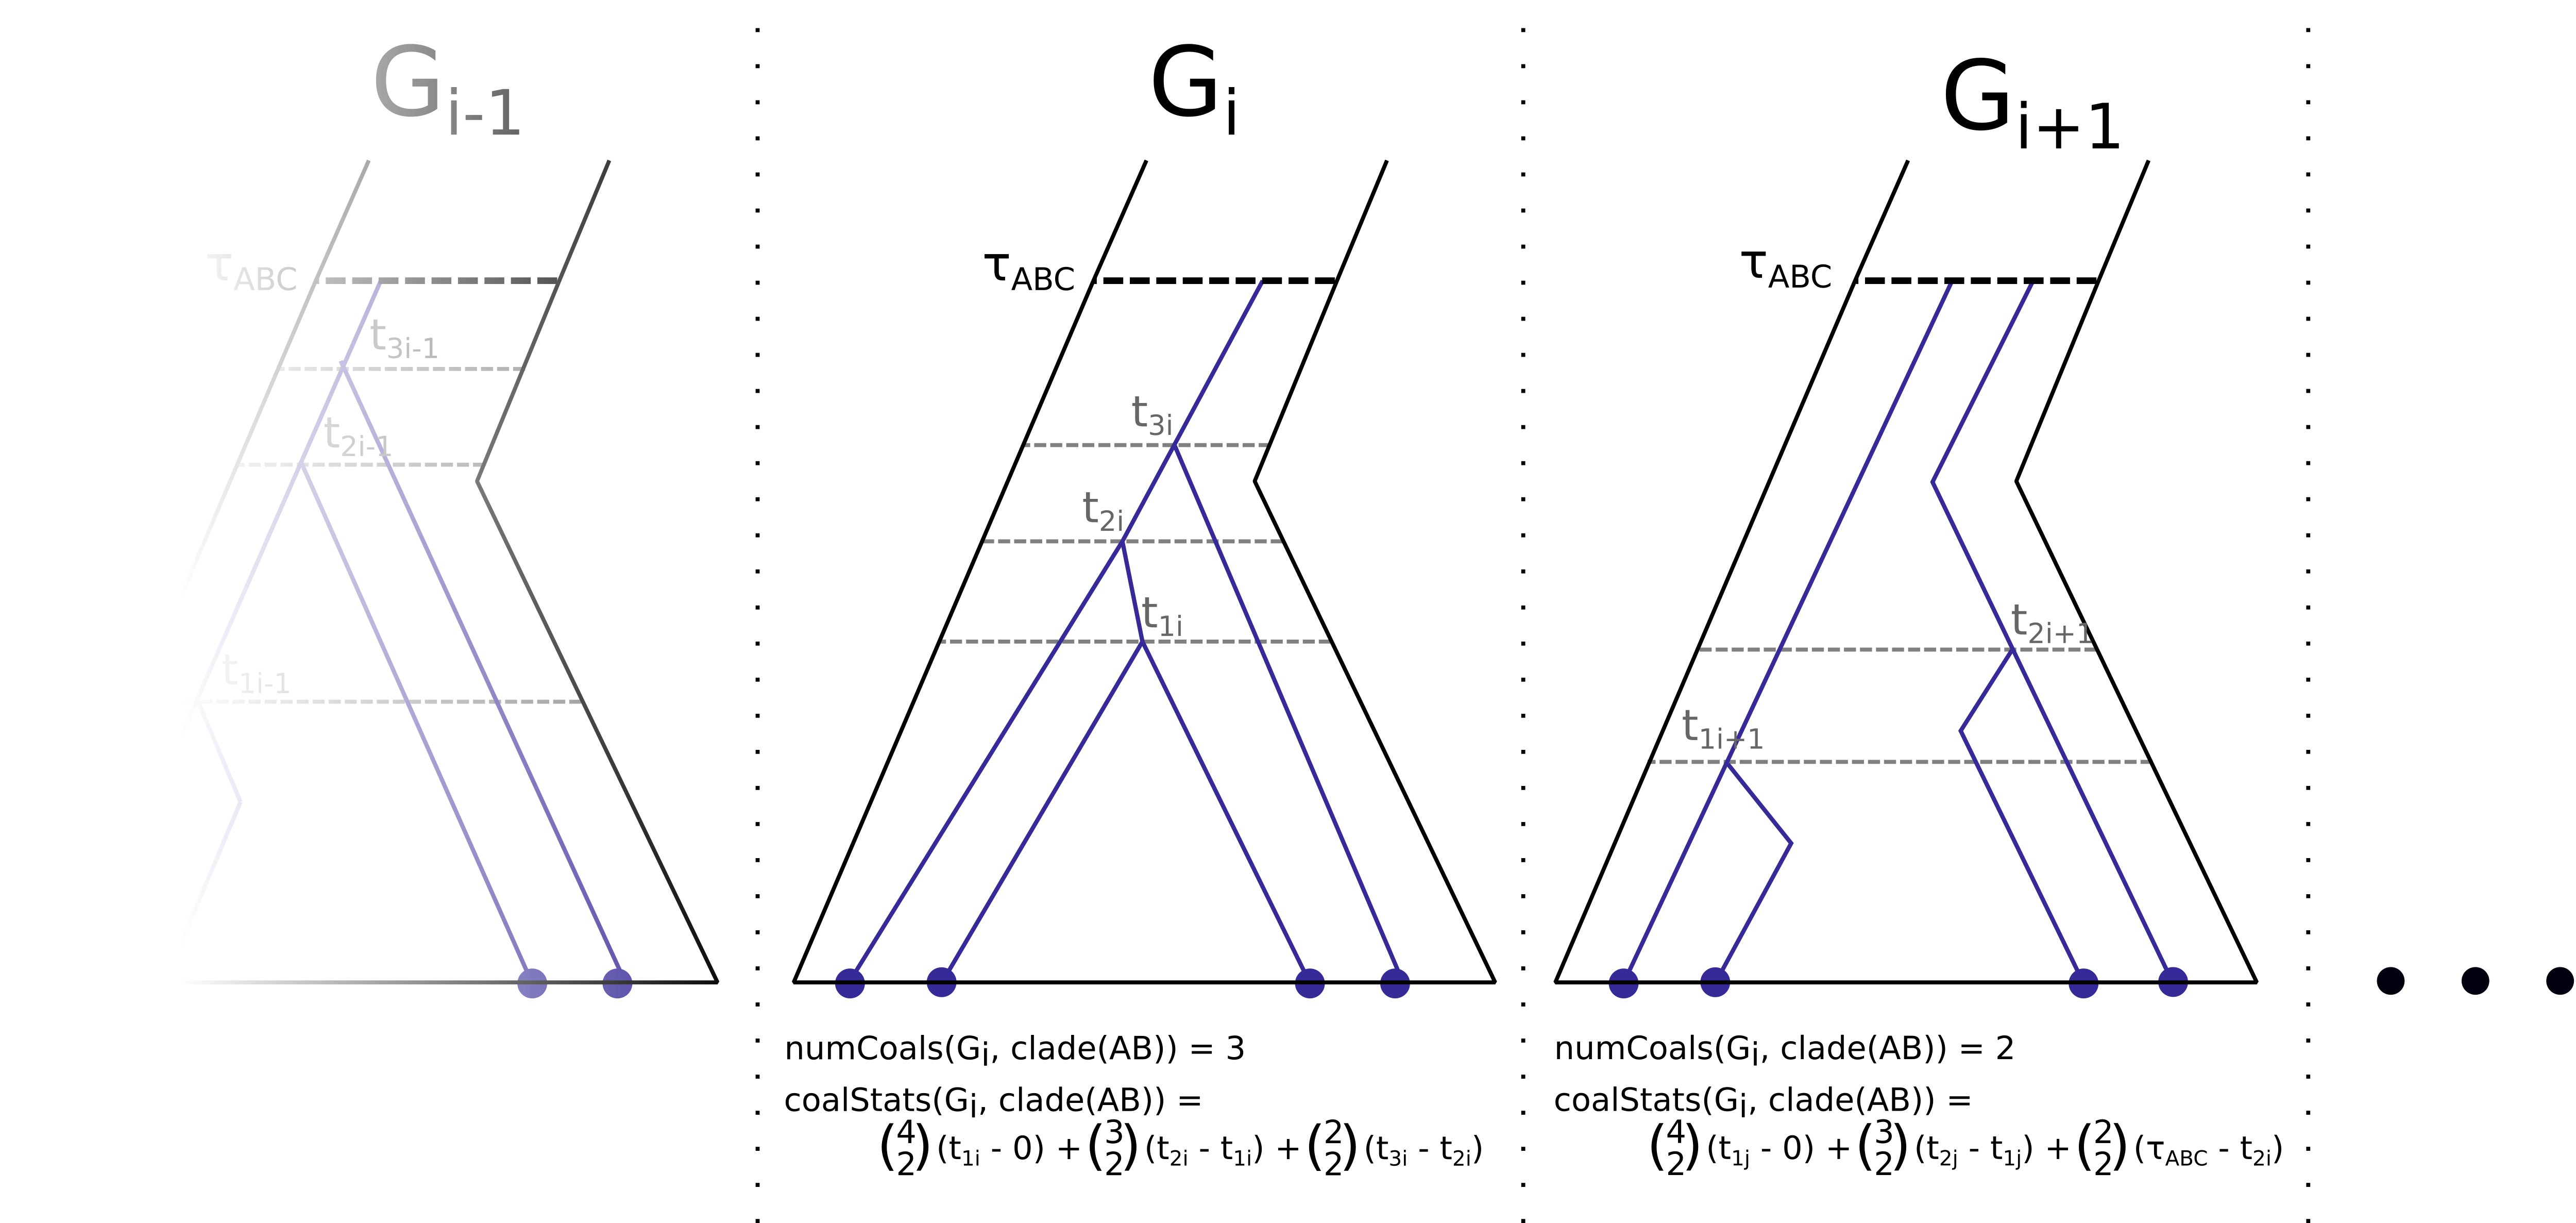
\includegraphics[width=1.0\textwidth]
{multiple_loci}
\captionsetup{width=.8\textwidth}
\caption{The sufficient statistic $coalStat(G, clade(AB))$ is calculated by accumulating the Kingman Coalescent genealogy log-likelihod across loci. The contribution of each locus is calculated via the set of intervals $\mathcal{I}(clade(AB),l_i)$. The sufficient statistic $numCoals(G, clade(AB))$ is simply the sum across loci of the amount of coalescnece events inside $clade(AB)$.
}
\label{fig:multiple_loci}
\end{figure}


The summary statistics $\{~numCoals(\G,p),~~ coalStats(\G,p)~\}_p$~ and ~$\{~numMigs(\G,b),~~ migStats(\G,b)~\}_b$ satisfy condition 3 in that their number depends on the complexity of the reference model $\Mref$ but not on the size of the data.
%
They also satisfy the second condition, because statistics computed for a given set of local genealogies and given values of divergence times enable computation of the likelihood $P(\G|\T,\Mref)$ for any set of values of the population size and migration rate parameters.


\subsection{Recursive Sufficient Statistics for All Clade Models}
\label{sec:Recursive Sufficient Statistics for All Clade Models}

To support all valid reference model structures generated by the reference construction process (subsection \ref{Constructing a Reference Model}) we must calculate the sufficient statistics for every population and migration band in every valid reference model -  \[\{~numCoals(\G,clade(p)),~~ coalStats(\G,clade(p))~\}_{p\in P_{ref}}\]

To efficiently achieve this, calculation of $numCoals$ and $coalStats$ is done recursively down the population phylogeny of $M$ as implemented in the pseudo-python code below. This implementation uses a function for computing $coalStats$ given a sorted list of intervals (function \pythoninline{calculate_coal_stats}), as well as accessors to data from \gp (functions \pythoninline{num_coals_from_gphocs} \& \pythoninline{sorted_intervals_from_gphocs}):
%

\begin{python}


def recursive_num_coals(pop):
    """recursively calculate and store num of coalescence
    events in clade(pop) as well as all descendant clades"""

    pop_num_coals = num_coals_from_gphocs(pop)

    if is_leaf(pop):
        return pop_num_coals

    left_num_coals = recursive_num_coals(pop.left)
    right_num_coals = recursive_num_coals(pop.right)

    current_num_coals = pop_num_coals + left_num_coals + right_num_coals
    store(current_num_coals)

    return current_num_coals


def recursive_coal_stats(pop):
    """recursively calculate and store coalescence stats
    of clade(pop) as well as all descendant clades"""

    pop_intervals = sorted_intervals_from_gphocs(pop)

    if is_leaf(pop):
        return pop_intervals

    left_intervals = recursive_coal_stats(pop.left)
    right_intervals = recursive_coal_stats(pop.right)
    merged_intervals = merge_sort(left_intervals, right_intervals)

    clade_intervals = merged_intervals.append(pop_intervals)

    clade_coal_stats = calculate_coal_stats(clade_intervals)
    store(clade_coal_stats)

    return clade_intervals

\end{python}

\subsection{Recursive Sufficient Statistics for All Comb Models}
\label{sec:Recursive Sufficient Statistics for All Comb Models}

Equation \ref{eq:gen_ratio_comb} shows how for a reference model created by comb-collapsing the root population, contribution of the genealogy-likelihood to the model-pairing conditional is reduced to contribution of the portion of genealogies above $\tmin$ - 
\[\frac{ P({\G}_{c|>\tmin}|\M_0,\theta_0=\troot) }{ P(\G_{>\tmin}|\M,\T)}\]

When comb-collapse is applied to a subtree, we apply the same idea to the portion of the genealogy contained in that subtree. Figure \ref{fig:calculate_hyp_stats_above_tmin} illustrates the intervals relevant for genealogy-likelihood calculation in the hypothesis and reference models. 


As in the case for clade reference models, we wish to calculate statistics for all viable comb reference models after only one MCMC chain. We do this by storing for every ancestral population $p$ the log of the denominator $~ln(P(\G_{>\tmin}|\M,\T))~$ and the two sufficient statistics involved in the calculation of the enumerator - ($\{~numCoals(\G,comb(p)),~~ coalStats(\G,comb(p))~\}_p$). 
%
This is again calculated recursively down the population phylogeny of $\M$, but the function \pythoninline{calculate_coal_stats} now takes into account only intervals inside the subtree of $p$ and above $\tmin$.


\begin{figure}[h]
\centering
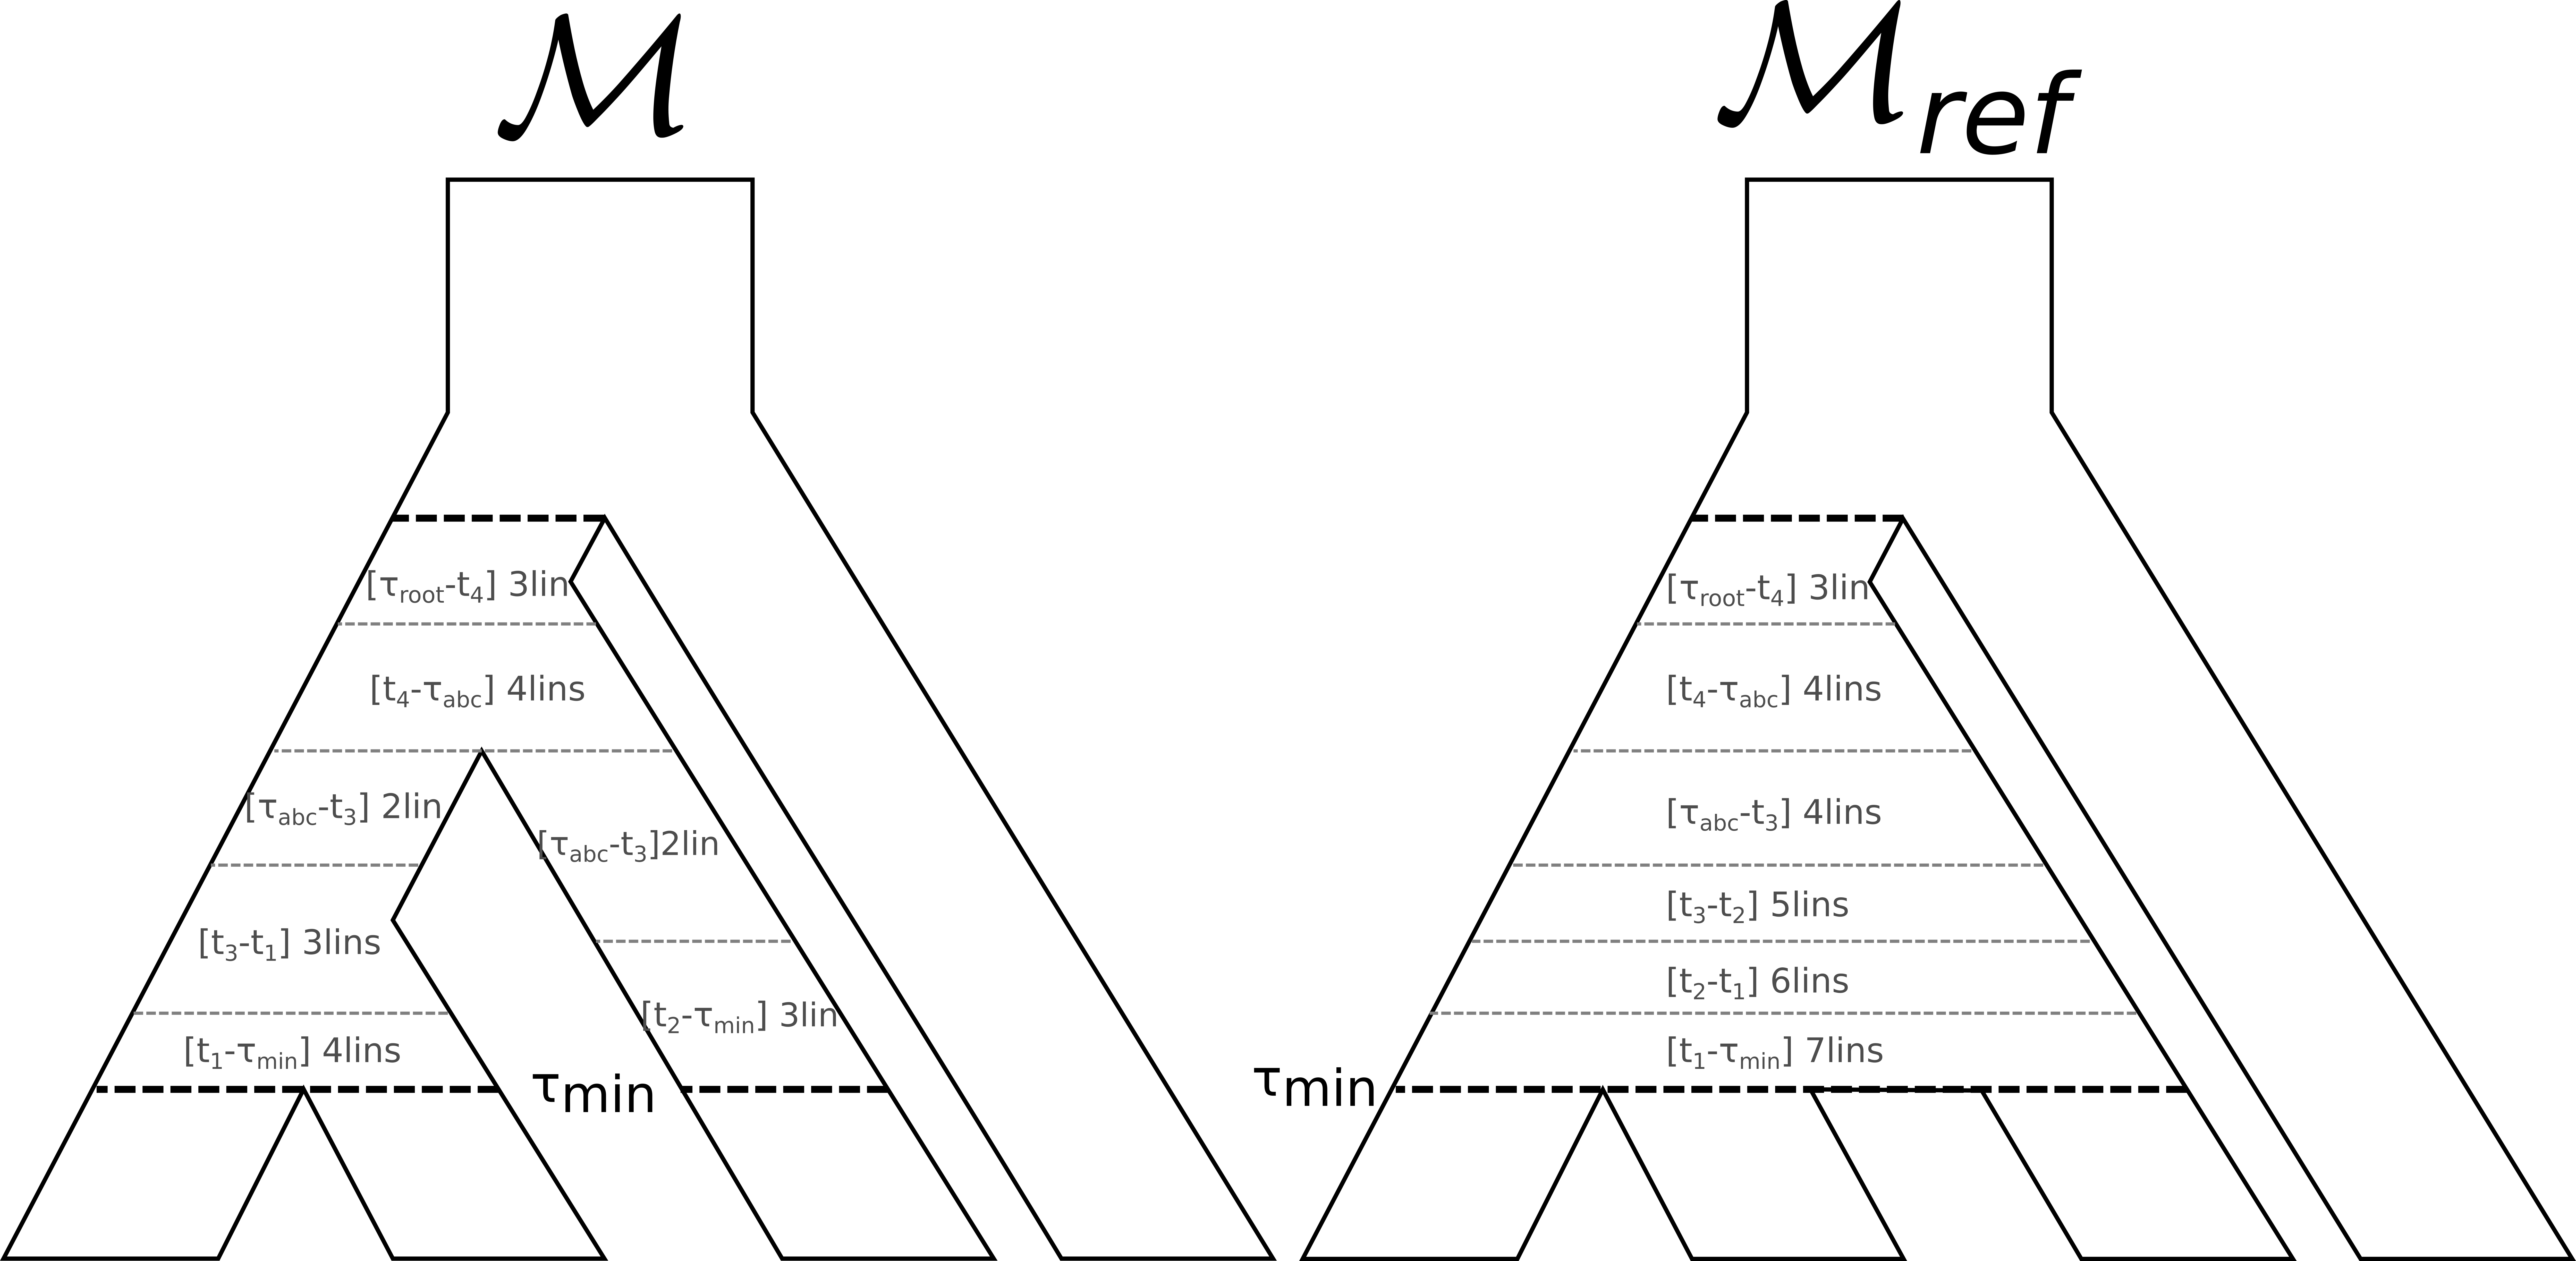
\includegraphics[width=1.0\textwidth]
{hyp_and_comb_intervals}
\captionsetup{width=.8\textwidth}
\caption{In comb reference models, genealogy-likelihood need only be calculated strictly within the bounds of the comb population $comb(p)$. Outside this area of the topology, genealogy-likelihood of the reference and hypothesis models cancels out in the Model-Pairing Conditional.}
\label{fig:calculate_hyp_stats_above_tmin}
\end{figure}


\subsection{Finalizing the RBF computation using McRef}
\label{sec:Finalizing the RBF computation}
After the MCMC process is completed, we are left with sufficient statistics and parameter priors per iteration for each clade and comb reference model. These are stored in multiple trace files (see example trace snippets in appendix \ref{ap:scripts}).
%
The only remaining step is to calculate the estimated relative model fit $P(X|\Mref)/P(X|\Mhyp)$ for a chosen reference model (or several). For this purpose we developed the McRef utility.

When setting up McRef, several parameters are configured. 
%
Chief among the configurations is the choice of reference model. This is specified by simply stating on what hypothesis population to perform a comb/clade collapse operation.
%
The remaining configuration options pertain to standard I/O (e.g. where the trace data files are stored and where to store output), to \gp configuration (e.g. what alpha \& beta to use for gamma priora, what print multipliers were applied to trace data when emitted by gphocs etc.), to internal statistical calculations (e.g. number of bootstrap iterations for confidence calculation and burn-in and sample-dilution in genealogy likelihood calculation) and to debugging (e.g. what debug calculations to run and visualizations to emit). 
%
See appendix \ref{ap:scripts} for an example configuration file.

McRef finishes calculating Equation \ref{eqn:ld-final} by plugging in the chosen parameters for each configured reference population. In our current implementation, $\theta_{root}$ of the comb/clade population in the reference model is set to the value of theta of the population at the root of the comb/clade in the hypothesis, but this can be easily adjusted if ever we decide to consider other theta mappings. 

With the goal of optimizing the practical run-time and usability of McRef, several techniques were employed; trace data files, which are repeatedly read and used, are lazily loaded and cached in each mcref process. Multiple McRef computations are launched using a single command-line tool and are cocurrently run in different processes, eventually aggregating summary results to a single log file. See appendix \ref{ap:scripts} for an example output.
%
To clarify results and to help in the understanding and debugging of mcref runs, several visualizations are emitted. Each mcref run emits plots of the genealogy-log-likelihood of the reference model and of the hypothesis model, as well as a plot of the rbf calculation across \gp iterations and a plot of the harmonic mean of likelihood of the hypothesis model. 
%
Multiple debug plots are also emitted by mcref. Their goal is to help the researcher assert the experiment was executed as planned. These plots contain the kingman coalescence and kingman migration of every population and migration in both the hypothesis and reference models. They also contain the aggregate coal-stats of the hypothesis and reference model. See appendix \ref{ap:scripts} for example debug graphs.



\section{Results}

In order to evaluate our new method we designed a series of experiments which measure it's strengths and weaknesses. 
%
The experiments were set up to try to distinguish between different hypothesis structures. 
%
Experiment 1 tries to decide whether a divergence did or did not occur. Experiment 2 tries to decide the ancestral relationship between three leaf populations and an out-group, and experiment 3 tries to identify the true migration pattern between leaf populations. 
%
We expect the RBF values to correlate with the degree of separation between different hypotheses.
%
A secondary goal of the experiment design is to learn how best to employ RBFs and how to choose a reference model for a given set of hypotheses.

\subsection{General Setup}
%
We generated data sets under different demographic scenarios, using the following constant setup. 
%
In experiments I and III, the generative population models (the "true" models) have 3 leaf populations $A$, $B$ and $C$, an ancestral population $AB$ and a root ancestral population $ABC$. 
%
In experiment II the true model has another ancestor population $ROOT$ which splits to $ABC$ and an outgroup leaf population $O$. 
%
We use the coalescent software \textit{ms} to generate four haploid sequences per leaf population. Sequence are comprised of 5000 loci of length 1000 bases. See appendix C for a sample file.
%
For each demographic scenario we generated two independent data sets (using the same generative hypothesis) to examine replication of results. 
%
To further assess replication we ran 2 independent MCMC runs in each G-PhoCS setting. See appendix \ref{ap:scripts} for an example \gp MCMC configuration file.


In each comparison instance we compared two hypothesis models $\M_1$ and $\M_2$ on a given data set. 
%
Depending on the specific test, comparison was done using relative Bayes factors with a differing reference model $\M_{ref}$ and using the harmonic mean for as a benchmark comparison. 
%
On each data set we ran \gp twice with $\M_1$ and twice with $\M_2$, yielding four potential differences between the relevant stats (e.g., $HM(\M_{\mathbf{1}}, data) - HM(\M_{\mathbf{2}},data)$, $RBF(\M_{\mathbf{1}}, \M_{null}, data) - RBF(\M_{\mathbf{2}}, \M_{null}, data)$). 
%
The differences represent the algorithms final "choice" between $\M_1$ and $\M_2$, i.e. which model has higher estimated data likelihood relative to the reference model.


For each comparison we recorded the maximum and minimum of the 4 differences with their standard error margins (which McRef computes via bootstrap). 
%
For the max value we recorded $max+ste$ and for the min value we recorded $min-ste$. Since the these errors correspond to the difference between two values, we took the square root of the sum of the two appropriate errors. 
%
As a result we attained 4 values for each comparison of $M_1$ and $M_2$ on a given data set and each method of comparison (e.g. $HM$, $RBF$ with null model, etc). We used these values to plot the confidence intervals seen in the following figures.


\subsection{Experiment I - Identifying Population Separation}
In this experiment we generated data sets for which population $ABC$s divergence time is fixed to 0.00300, and perturbed $AB$s divergence time from 0 up to 0.00050. No migration was allowed between any population. We considered 2 hypotheses:
%
\begin{enumerate}
\item $\M_{3pops}$ - A model with 3 leaf populations $A$, $B$ and $C$. This is the true model used to generate the sequence data
\item $\M_{2pops}$ - A model with 2 leaf populations $AB$ and $C$, where the sequenced individuals of the original $A$ and $B$ populations are grouped into a single leaf population $AB$. This model coincides with the true model in the data set with $\tau_{AB}:=0$
\end{enumerate}
%
and compared these two models using each of three techniques:
%
\begin{enumerate}
\item The harmonic mean
\item Relative Bayes factors with a reference model of $\M_{null}$
\item Relative Bayes factors with a reference model of $\M_{clade(AB)}$ (the original model with a clade rooted at population $AB$). Note that when $\Mhyp := \M_{2pops}$ we get $\Mref=\Mhyp$
\end{enumerate}


We used these three techniques to compare models $\M_{3pops}$ and $\M_{2pops}$ (i.e., $\log{\frac{P(X|\M_{3pops})}{P(X|\M_{2pops})})}$) with each variant of the data set.



\begin{figure}[h]

\figuretitle{Selecting between $\M_{3pops}$ vs $\M_{2pops}$ using RBFs or HM}


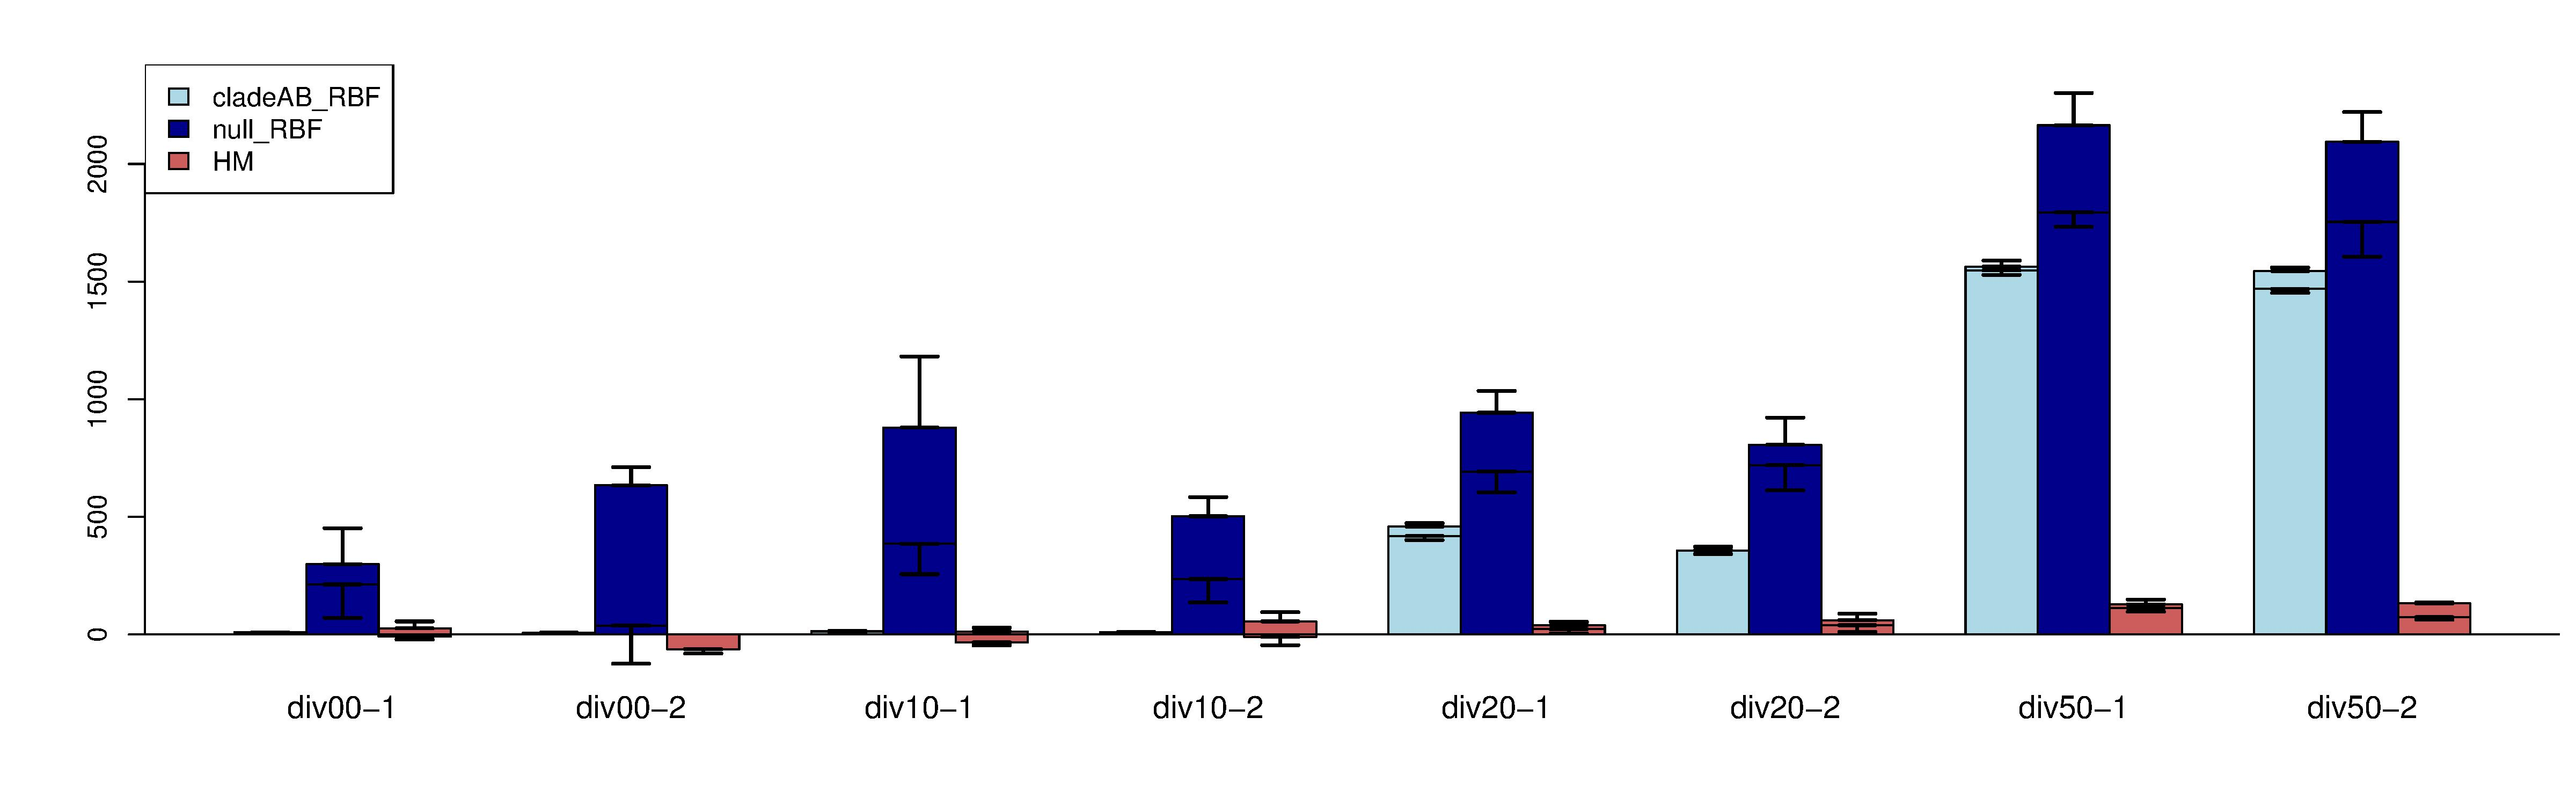
\includegraphics[scale=0.4]{results/results-divAB-select}
\captionsetup{width=0.8\textwidth}
\caption{
Data sets are marked on the X-axis by divXX-a, where the value of $XX$ stands for $\tau_{AB} \times 10,000$ and $a$ indicates the data replicate (1 or 2).
%
The divergence time of $AB$ used in the generation of the data set increases between comparisons (left to right).
%
The bars heights are the values of the comparison metric $\log{\frac{P(X|\M_{3pops})}{P(X|\M_{2pops})}}$.
%
Each experiment was repeated twice to assess reproducability. We see in the graph that for $\tau_{AB} \leq 0.00020$ the harmonic mean does not confidently prefer the true hypothesis $\M_{3pops}$ over the competing hypothesis $\M_{2pops}$.
%
RBFs, however, prefer $\M_{3pops}$ starting from $\tau_{AB} \geq 0.00010$, regardless of the chosen reference model.
%
}
\label{fig:results-divAB}
\end{figure}


First, we observe that when computing $RBF(\Mhyp=\M_{2pops}, \Mref=\M_{clade(AB)}$, we get values near 0 ($<1e^{-6}$). This is because the reference and hypothesis models converge to the same model. We consider this a simple validation of our RBF calculation. 
%
We also notice that both HM and the two RBFs are able to determine the correct model ($\M_{3pops}$) for $div\-50$, and they don't reject $\M_{2pops}$ for $div\-00$ (although $null\_RBF$ does give positive values). 
%
In $div\-20$ we see that both RBFs determine the correct model, while the harmonic mean does not significantly reject $\M_{2pops}$.
%
Lastly, when we use $\Mref = \M_{clade(AB)}$, we see that the estimates of RBF are much less noisy than when using $\Mref = \M_{null}$.
%
Also, the added noise for $\M_{null}$ appears to bias upward the RBF estimates, resulting in false-positives for low divergence data sets ($div\-00$ and $div\-10$).



\subsection{Experiment II - Determining model topology}
In this experiment the true model contained an additional outgroup leaf population $O$. The divergence time of population $ROOT$ to $O$ and $ABC$ was set to 0.01000. The divergence time of $ABC$ was again fixed to 0.00300 and the divergence time of $AB$ was perturbed between 0.00300 and 0.00180. Again, no migration was allowed between any population. We considered 3 hypotheses:
%
\begin{enumerate}
\item $\M_{AB\_C}$ - A model with four leaf populations $A$, $B$ and $C$ and $O$ where $A$ and $B$ are siblings. This is the true model used to generate the sequence data
\item $\M_{A\_BC}$ - A similiar model but in which $B$ and $C$ are siblings
\item $\M_{AC\_B}$ - A similiar model but in which $A$ and $C$ are siblings
\end{enumerate}
%
Note that when $\tau(AB) = 0.00300 = \tau(ABC)$, the simulated model is one in which  the three populations instantaneously diverge, so we expect the three hypothesis models to have similiar fit to data. We compared these models using each of five techniques:
%
\begin{enumerate}
\item The harmonic mean
\item Relative Bayes factors with a reference model of $\M_{Clade(ROOT)} = \M_{null}$
\item Relative Bayes factors with a reference model of $\M_{Clade(ABC)}$
\item Relative Bayes factors with a reference model of $\M_{Comb(ROOT)}$
\item Relative Bayes factors with a reference model of $\M_{Comb(ABC)}$
\end{enumerate}


Similiarly to experiment I, we used these techniques to compare the true model $\M_{AB\_C}$ against the alternatives $\M_{A\_BC}$ and $\M_{AC\_B}$. Figures \ref{fig:results-M4-divAB-comb}-\ref{fig:results-M4-divAB-HM} show the results of the comparisons.



\begin{figure}[H]

\figuretitle{Comparing performance of multiple reference models and HM}

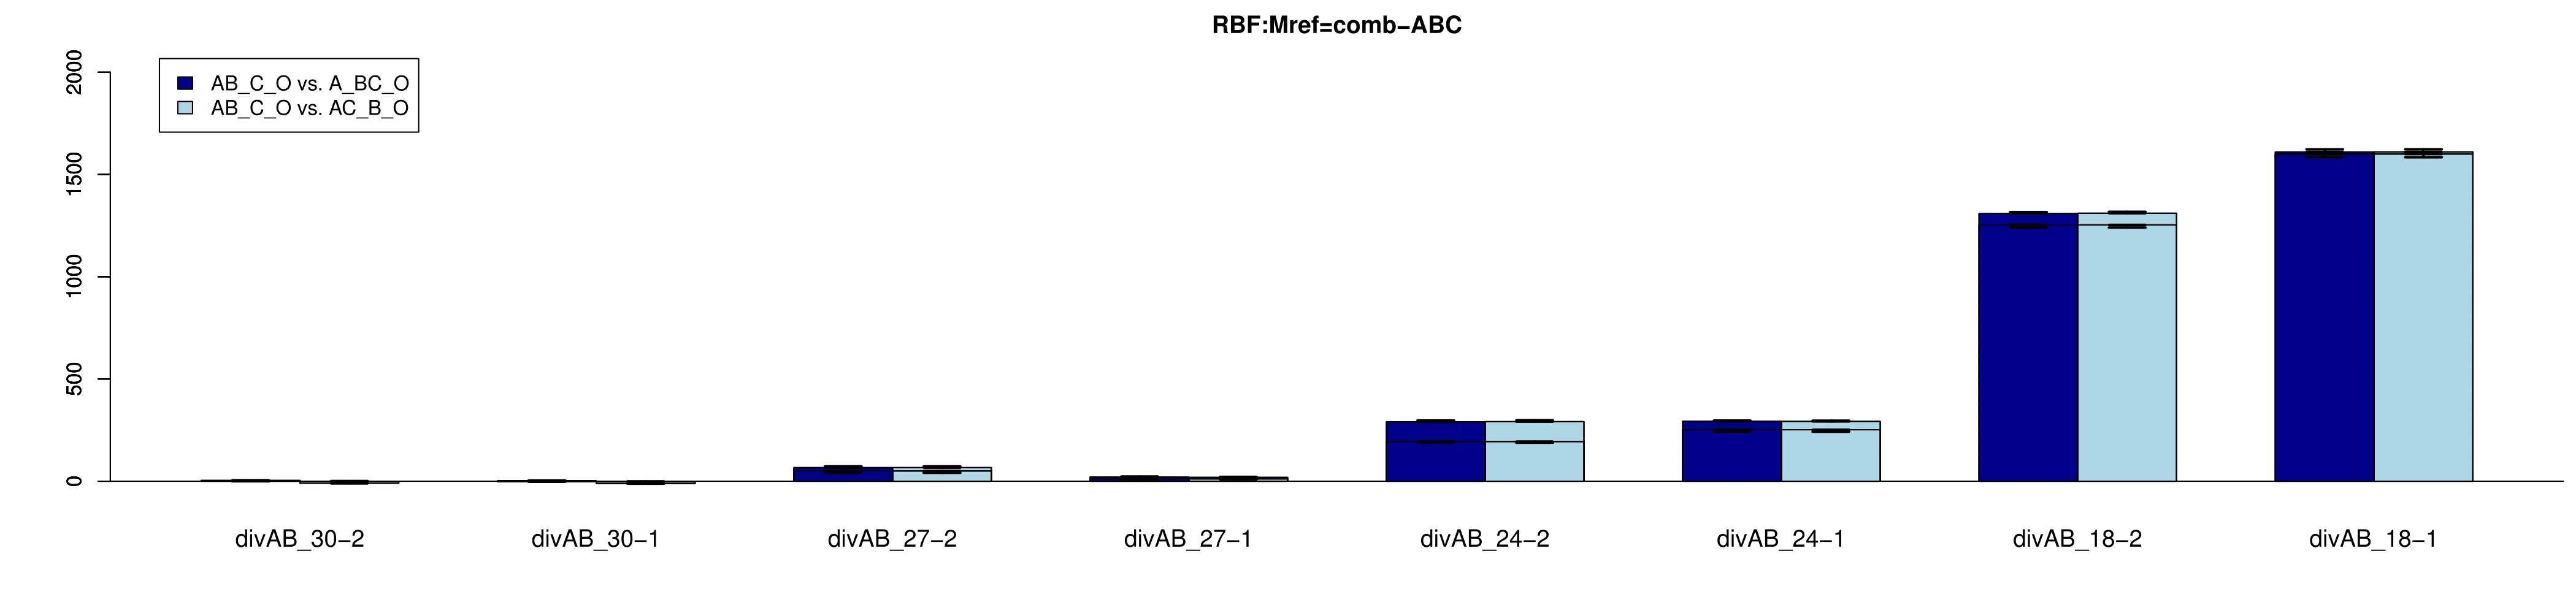
\includegraphics[width=1.0\textwidth]{results/results-M4-divAB/M4-divAB-results-comb_ABC}

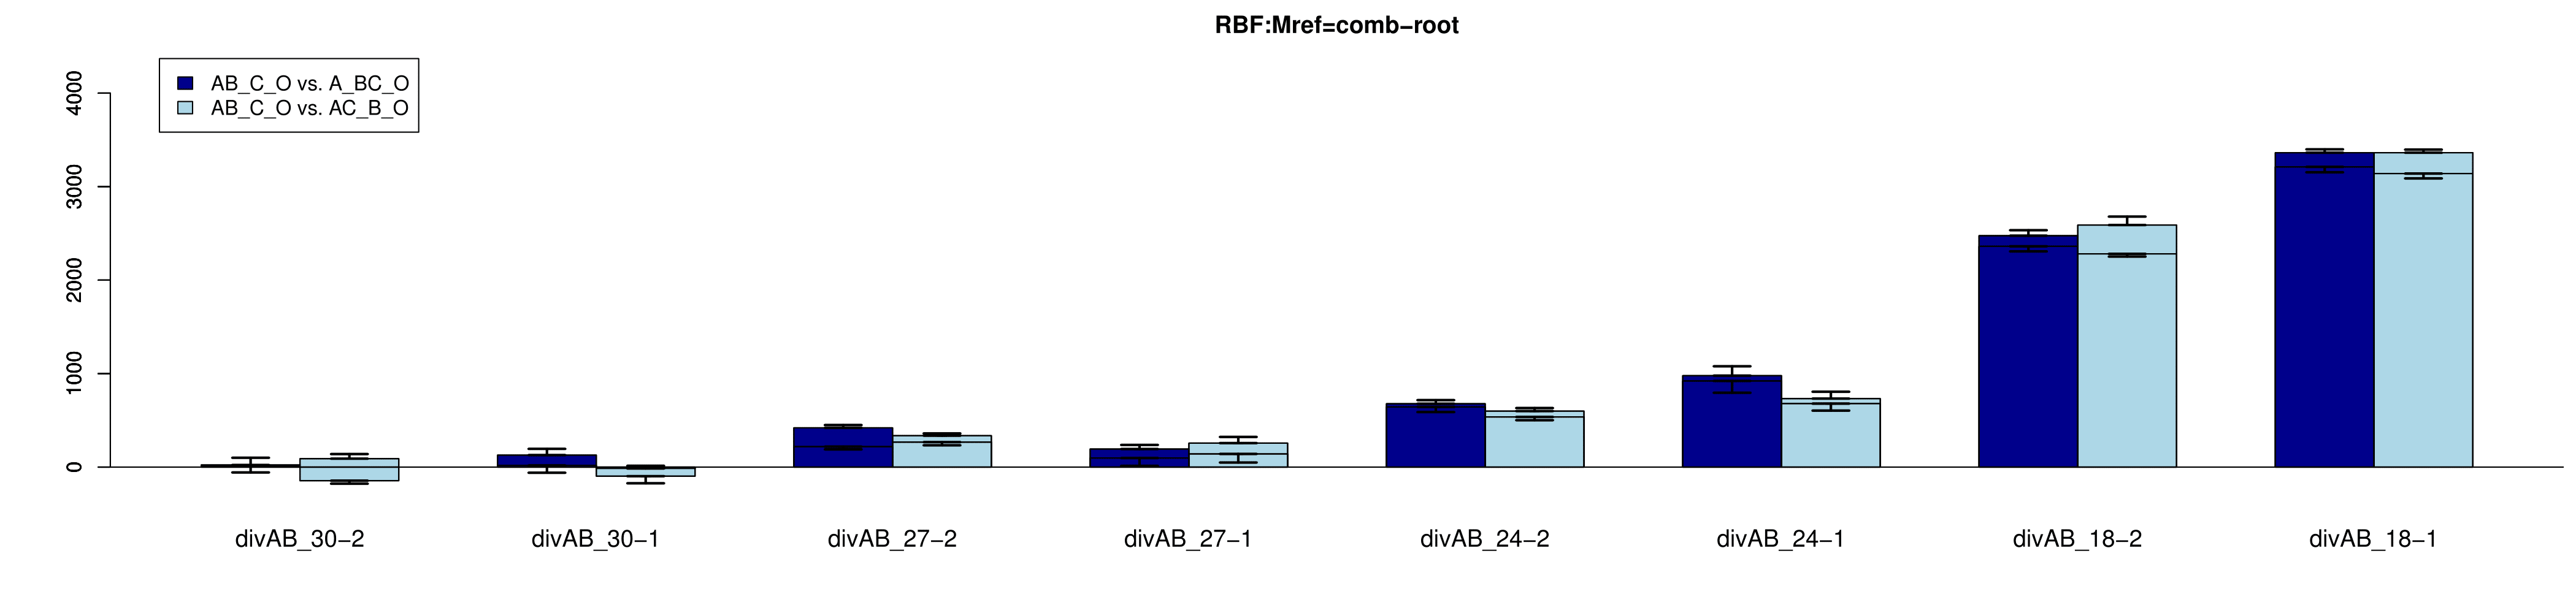
\includegraphics[width=1.0\textwidth]{results/results-M4-divAB/M4-divAB-results-comb_ROOT}

\captionsetup{width=0.8\textwidth}
\caption{ 
Data sets are marked on the X-axis by $divAB\_XX-a$, where the value of $XX$ stands for $\tau(AB) \times 10,000$ and $a$ indicates the data replicate (1 or 2).
%
The true gap between divergence times $\tau(ABC)$ and $\tau(AB)$ starts from zero on the left (where $\tau(ABC) = 0.00300 = \tau(AB)$) and increases between comparisons (left to right).
%
We clearly see from figures \ref{fig:results-M4-divAB-comb} -  \ref{fig:results-M4-divAB-HM} that the more specialized reference models ($Comb(ABC)$ followed by $Comb(ROOT)$) successfully select the true model, whereas the  more general methods are very noisy and uncertain, even when the hypotheses should be indistinguishable.}
\label{fig:results-M4-divAB-comb}
\end{figure}

\begin{figure}[H]
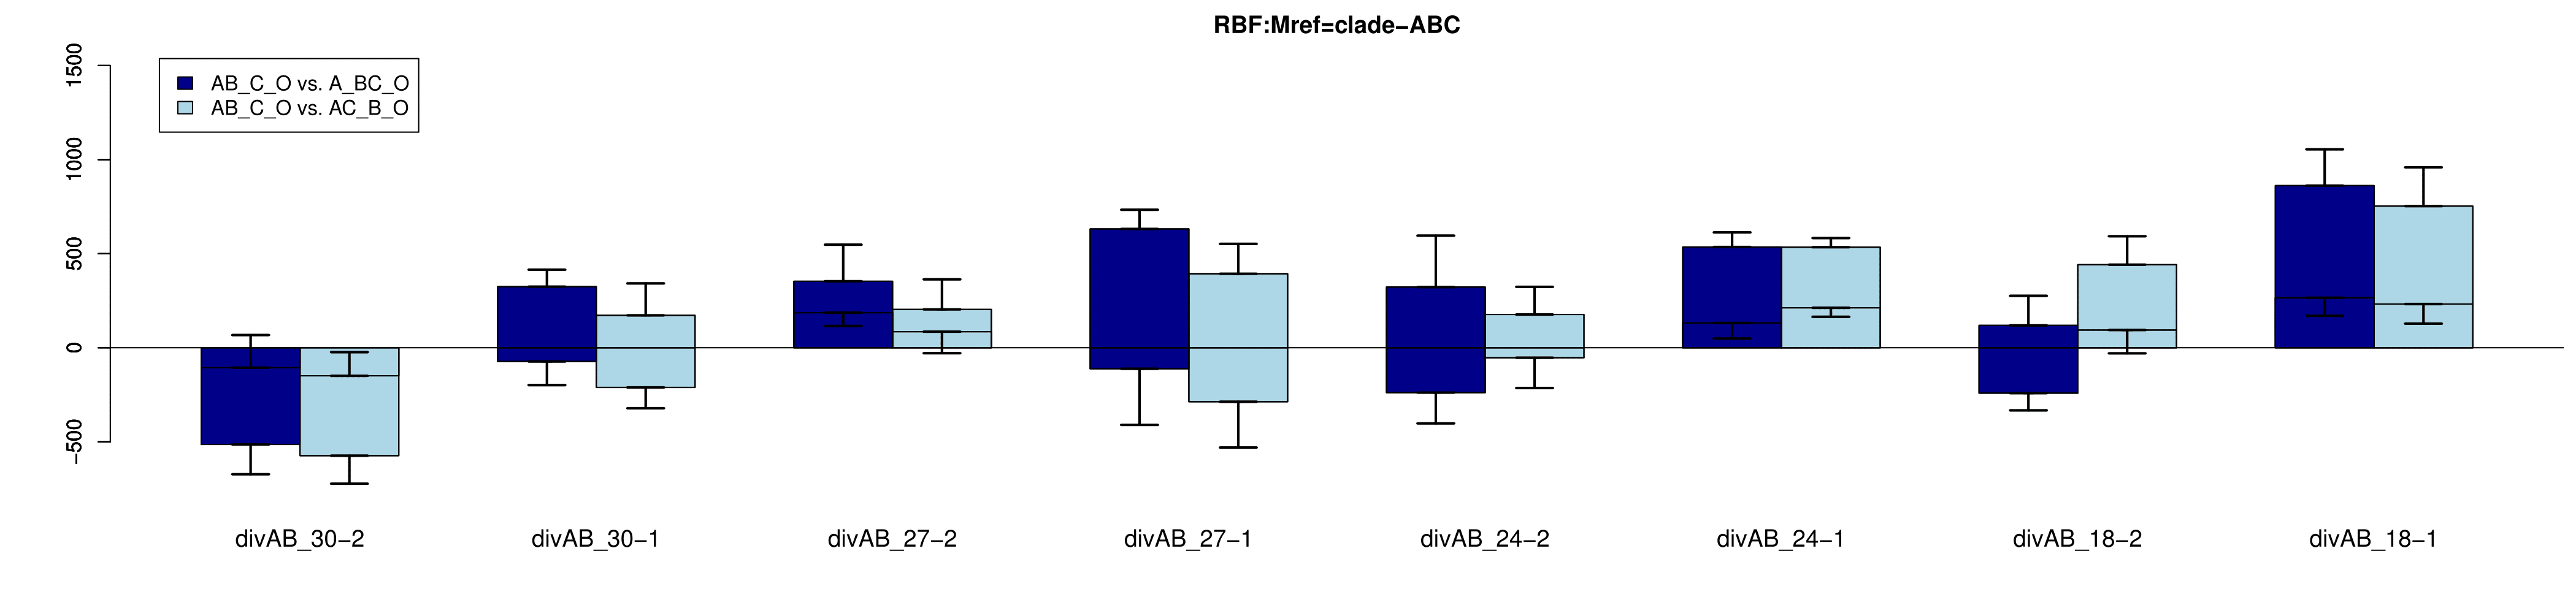
\includegraphics[width=1.0\textwidth]{results/results-M4-divAB/M4-divAB-results-clade_ABC}
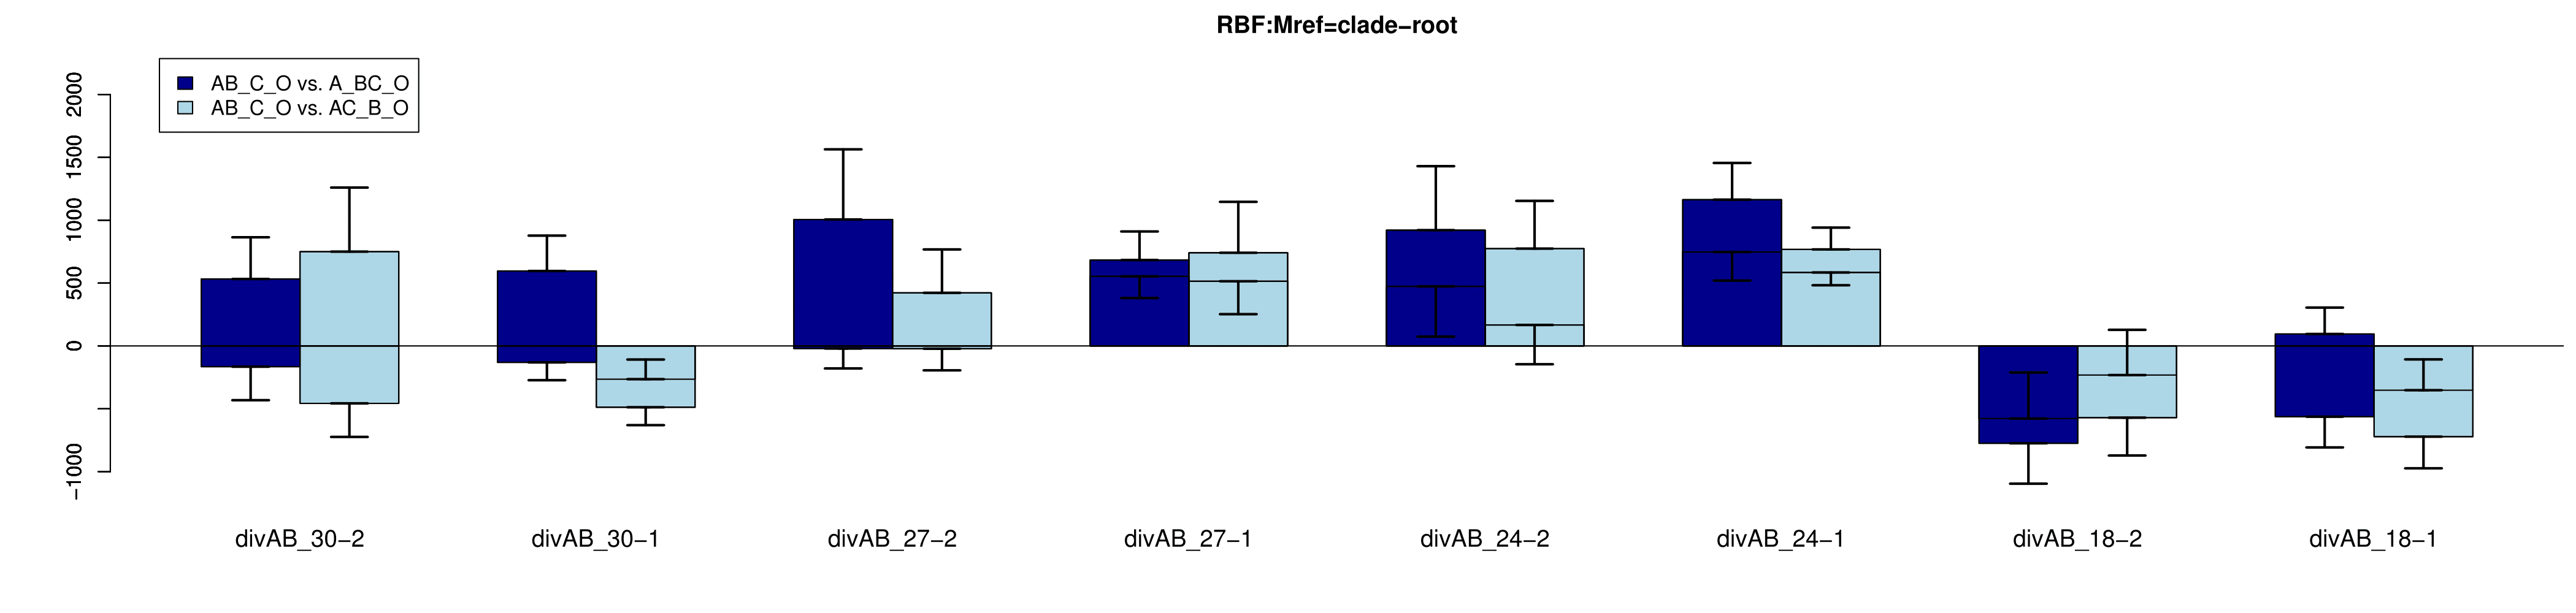
\includegraphics[width=1.0\textwidth]{results/results-M4-divAB/M4-divAB-results-clade_ROOT}
\caption{ }
\label{fig:results-M4-divAB-clade}
\end{figure}

\begin{figure}[H]
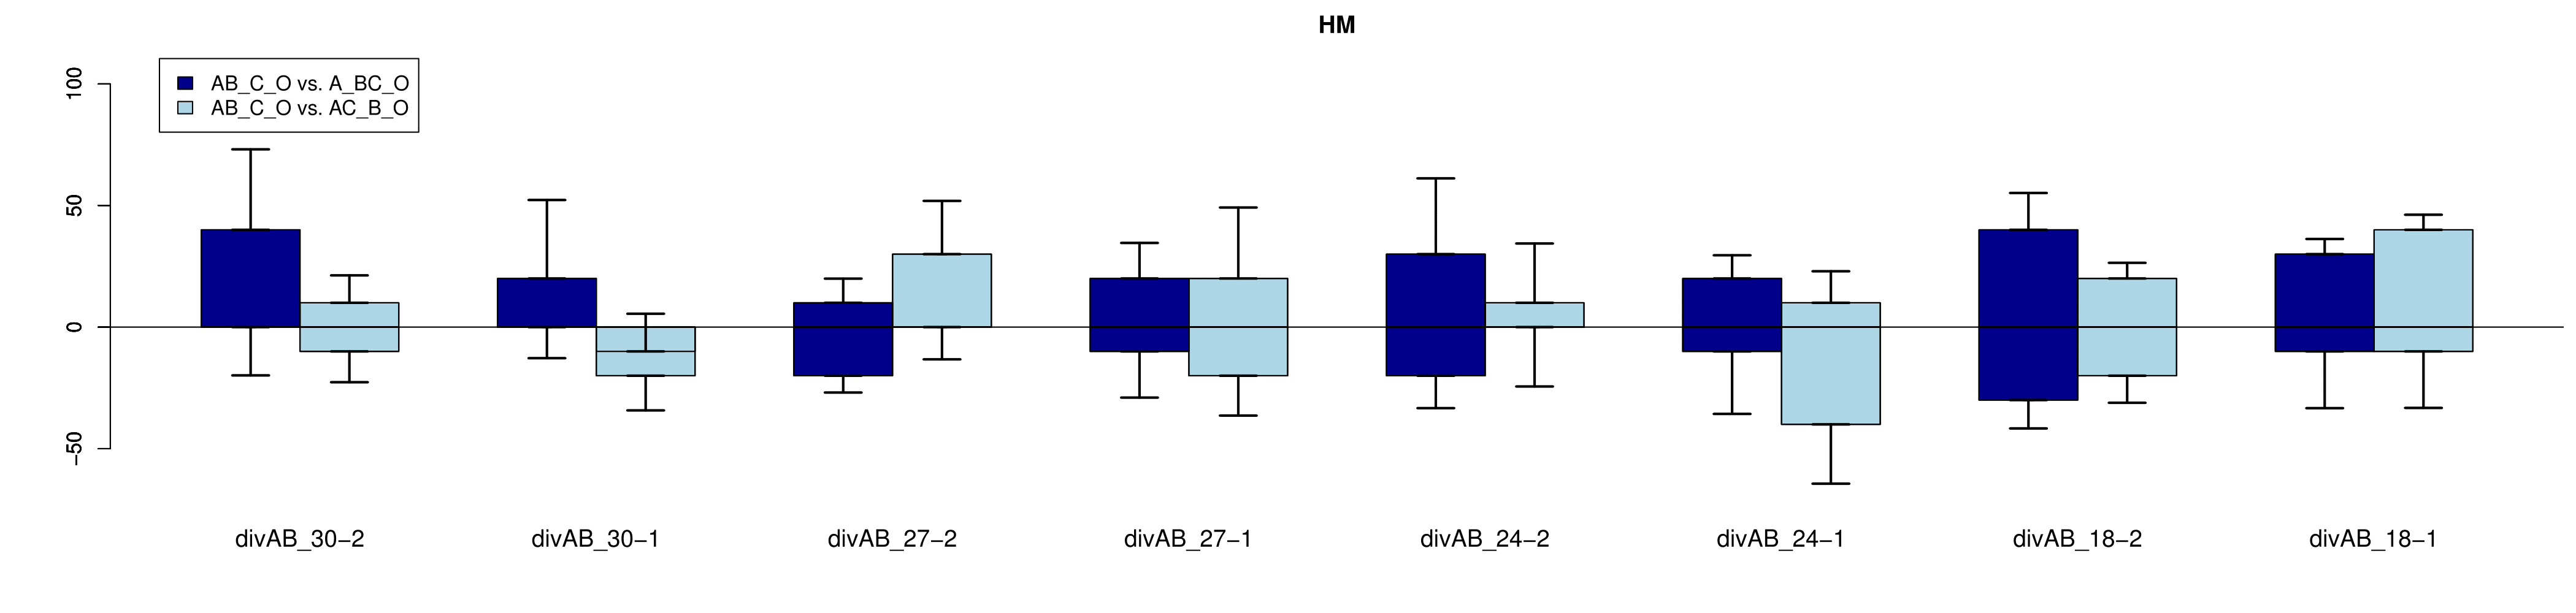
\includegraphics[width=1.0\textwidth]{results/results-M4-divAB/M4-divAB-results-HM}
\caption{ }
\label{fig:results-M4-divAB-HM}
\end{figure}

As seen in figure \ref{fig:results-M4-divAB-comb}, the two comb reference methods clearly and confidently choose the true hypothesis model, $\M_{AB_C}$.
%
The comb reference methods also correctly show no preference to any model when the hypotheses were eqivalent. This is not true for the other methods.
%
Amongst the two comb reference methods, the more localized $Comb(ABC)$ provided a stronger and more confident signal.
%
However, when using the $Clade(ABC)$ reference model (top of figure \ref{fig:results-M4-divAB-clade}) we see at most a gentle upward trend in results, but no reproducable clear selection. 
%
In the remaining two experiments ,$Clade(ROOT)$ and HM (figures \ref{fig:results-M4-divAB-clade} and \ref{fig:results-M4-divAB-HM}) we see no selection and a high degree of uncertainty.



\subsection{Experiment III - Determining direction of gene flow}
In this experiment we generated data sets where the divergence times are fixed to $\tau_{ABC} = 0.00300$, and $\tau_{AB} = 0.00150$ and simulated different migration rates from population $C$ to population $B$.
%
We considered four hypotheses:
\begin{enumerate}

\item $\M_{migCB}$ - A model with a migration band from $C$ to $B$ (the true model)

\item $\M_{nomig}$ - A model with no migration bands

\item $\M_{migALL}$ - A model with migration bands between all pairs of sampled populations (6 migration bands total)

\item $\M_{migBC}$ - A model with migration band from $B$ to $C$

\end{enumerate}
%
and examined two ways to compare these 4 models:
\begin{enumerate}
\item Using the harmonic mean estimator (HM)
\item Using RBF where $\Mref = \M_{null}$

\end{enumerate}

To present the results, we conducted a comparison between each of the three models with migration against $\M_{nomig}$ as a base model (e.g. $\log{ \frac{P(X|\M_{migBC})}{P(X|\M_{nomig})}}$). 
%
We ploted for each data set and each model with migration the 4 values associated with this comparison, under $null\_RBF$ (Figure \ref{fig:results-migCB-1}) and the harmonic mean (Figure \ref{fig:results-migCB-2}). 
%
Because the conditional distribution for migration events is not fully implemented, we applied a small shortcut and assumed the hypothesis and reference likelihoods cancel out. We estimate that this results in a relatively small correction, and believe strong trends in results will not be affected by this.



\begin{figure}[H]

\figuretitle{Selecting between $\M_{migALL}$ vs $\M_{migCB}$ vs $\M_{migBC}$ using HM}

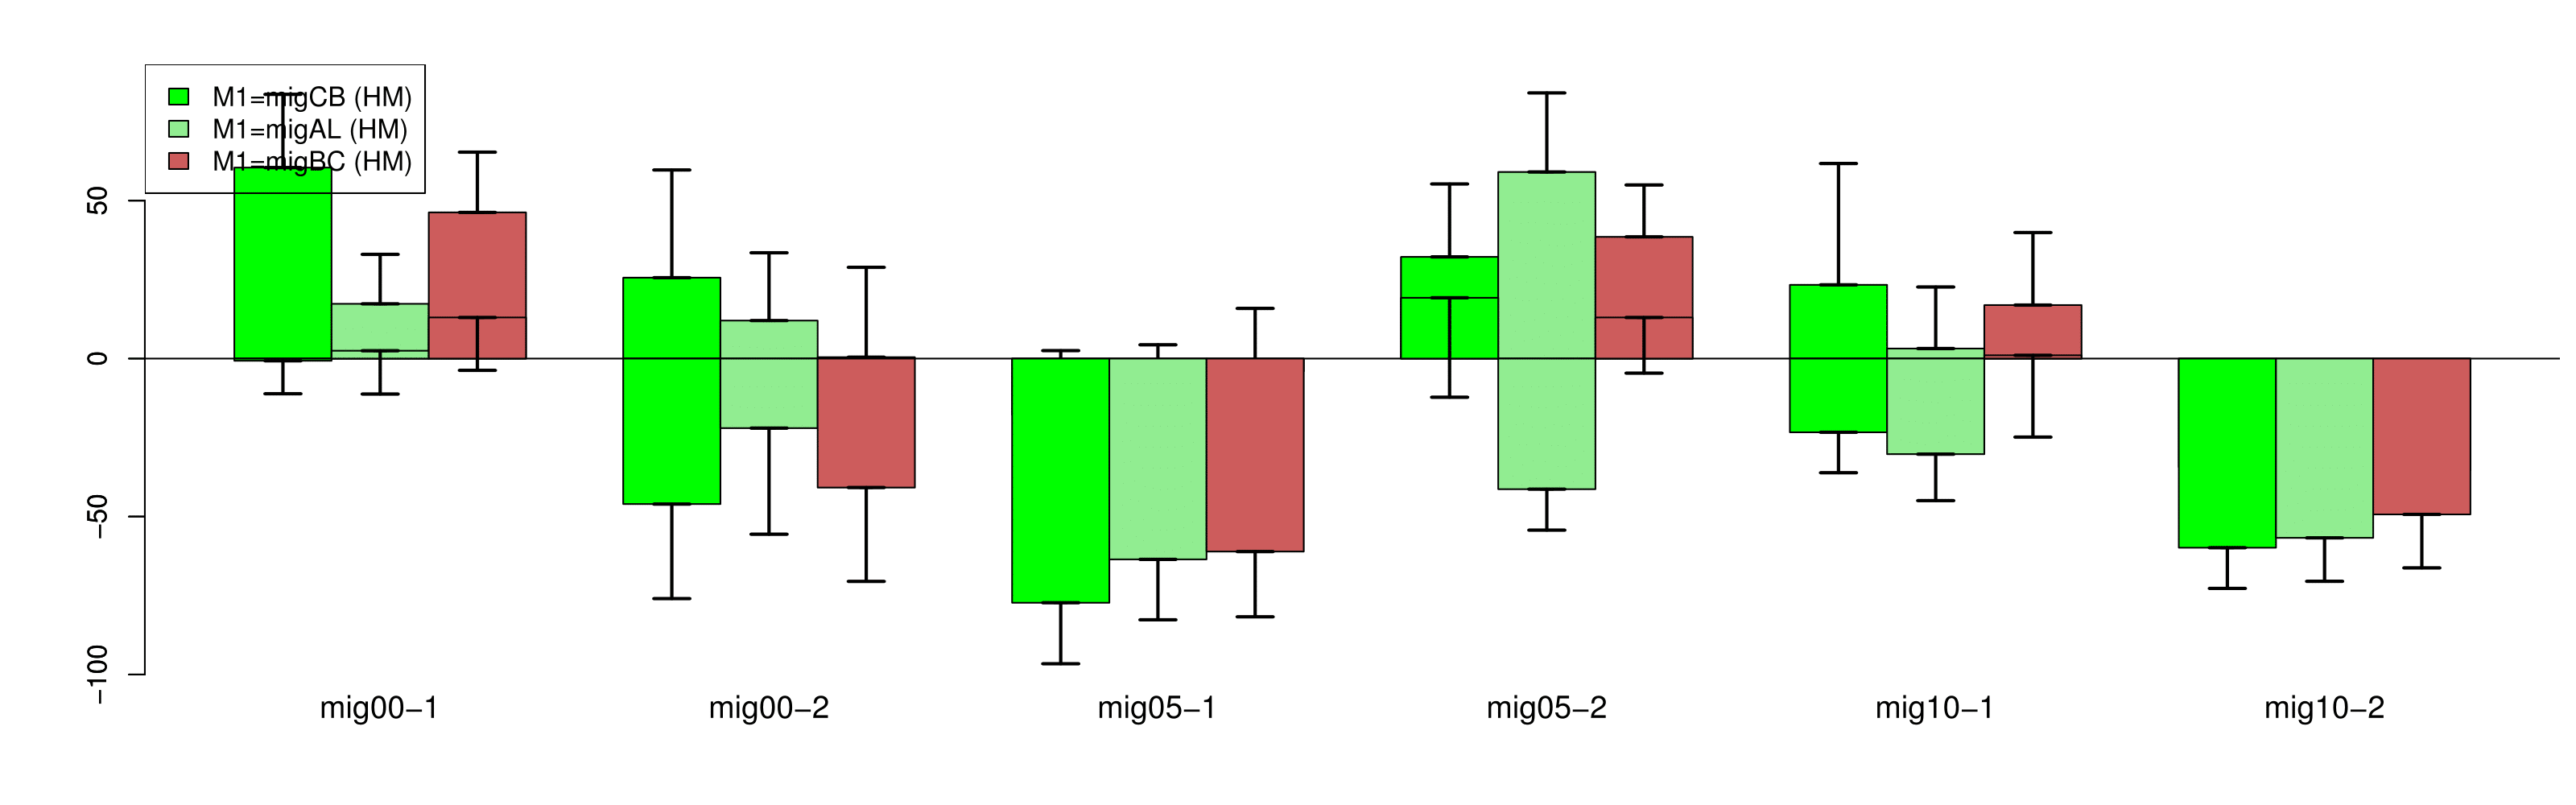
\includegraphics[width=1.0\textwidth]{results/results-migCB-select-2}
\captionsetup{width=1.0\textwidth}
\caption{
Data sets are marked by $migXX-a$, where $XX$ stands for the migration rate from population $C$ to $B$ and $a$ indicates the data replicate (1 or 2).
%
The migration rate from $C$ to $B$ used in the generation of the data set increases between comparisons (left to right).
%
The bars heights are the values of the comparison metric against $\M_{nomig}$ , e.g. $\log{ \frac{P(X|\M_{migBC})}{P(X|\M_{nomig})}}$.
%
Each experiment was repeated twice to assess reproducability.
%
We see in the graph that the harmonic mean does not consistently prefer any model over another.
}
\label{fig:results-migCB-2}
\end{figure}



\begin{figure}[H]

\figuretitle{Selecting between $\M_{migALL}$ vs $\M_{migCB}$ vs $\M_{migBC}$ using RBF with $\M_{null}$}


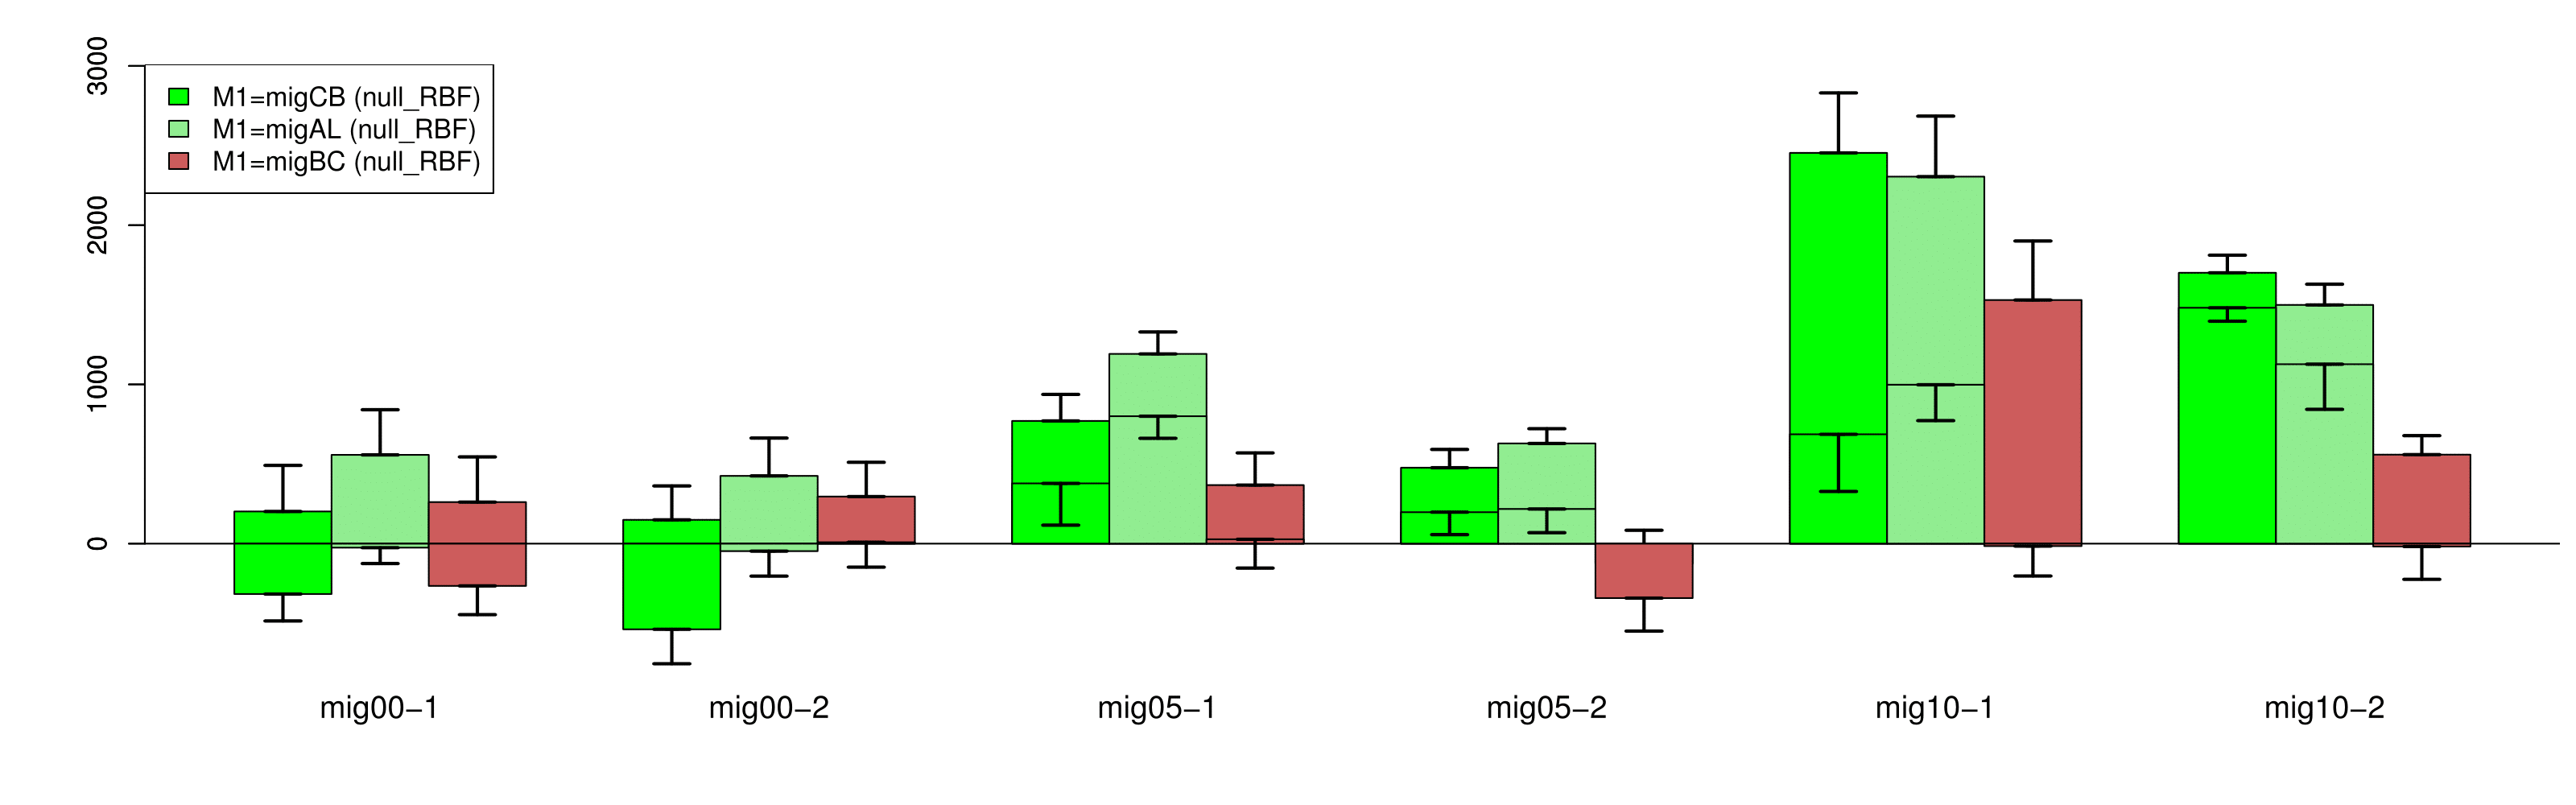
\includegraphics[width=1.0\textwidth]{results/results-migCB-select-1}
\captionsetup{width=1.0\textwidth}
\caption{
As opposed to in figure \ref{fig:results-migCB-2}, we see that the RBF prefers models with migration to the migration-less base model. 
%
This preference is correlated with migration rate. 
%
We also see that RBF using a comb reference model produces estimates with higher confidence.
}
\label{fig:results-migCB-1}
\end{figure}



In figure \ref{fig:results-migCB-2} we see that the harmonic mean scores the three models with migrations similarly and it never significantly prefers models with migration to $\M_{nomig}$.
%
RBFs however consistently score $\M_{migCB}$ and $\M_{migAL}$ higher than $\M_{nomig}$ in the 4 data sets with migration. The preference is correlated to the simulated migration rate. 
%
RBFs also score $\M_{migCB}$ and $\M_{migALL}$ higher than $\M_{migBC}$. This shows that they are able to identify the direction of migration ($C\rightarrow B$ instead of $B \rightarrow C$).
%
There doesn't seem to be a significant difference between the scores of $\M_{migCB}$ and $\M_{migALL}$. In principle, we would've liked to give a higher score to the most "compact" model, but this is not attained.



\subsection{summary}

We've examined RBFs under three questions - 1) whether a divergence event occured, what is the migration pattern and what is the relationship between leaves. In all three scenarios, model selection using relative Bayes factors significantly outperform the harmonic mean estimator
%
We've also shown (in experiment 2) that the choice of reference model has a great impact on algorithm performance. Generaly speaking, the more localized the reference model is to the disputed hypothesis region, the better the algorithm performed. 
%
We see that , as expected, the success of the algorithm is correlated with the true distance between models, but it's estimations are not of high certainty.
%
Finally we note that it did not succeed in choosing the more parsimonious hypothesis in experiment 3 leaving room for improvement.


\newpage

\newpage

\section{References}
\renewcommand*{\refname}{ }
\bibliographystyle{mbe}
\bibliography{compbio}



\newpage


\appendix
\newcommand{\anc}{\geq_\Tr}
\newcommand{\nanc}{\ngeq_\Tr}

\section{\texorpdfstring{The conditional distribution $\Pref(\taus|\G)$ for models without migration}{Conditional distribution without migration}}\label{ap:cond_nomig}

When the hypothesis model $\M$ has no migration, its model-pairing conditional distribution with the null model $\M_0$ is determined by specifying a conditional
distribution for the divergence times, $\Pref(\taus|\G)$, such that $\Pref(\taus|\G)>0$ if and only if $P(\G|\taus,\M)>0$
(see Equations \ref{eq:pref_support} and \ref{eq:rbf_null}).
%
Let $(\Tr,\taus)$ be a timed population phylogeny and let $\G$ be a collection of coalescent trees in which every leaf is mapped to a leaf population in $\Tr$
and  every internal vertex $v$ corresponds to a coalescent event at time $t(v)$.
Then $P(\G|\taus,\M)>0$ if and only if the trees in $\G$ can be \emph{embedded} in  $(\Tr,\taus)$, as defined below.
%
\begin{definition}\label{def:embed}
 An embedding of a collection of local genealogies $\G$ in a timed population phylogeny $(\Tr,\taus)$ is a mapping, $pop:\G\rightarrow\Tr$,
 which satisfies the following conditions for every coalescence event $v\in\G$:
 \begin{enumerate}
  \item $pop(v)$ is alive at time $t(v)$:~~ $\tau(pop(v)) ~<~ t(v) ~\leq~ \tau(parent(pop(v)))$~.\label{cond:time}\\
  (if $p$ is a leaf population then $\tau(p)=0$ and if $p$ is the root population then $\tau(parent(p))=\infty$.)
  \item $pop(parent(v))$ is ancestral (or equal) to $pop(v)$:~~ $pop(parent(v)) \anc pop(v)$.\label{cond:anc}
 \end{enumerate}
\end{definition}

% Note that condition \ref{cond:anc} can be extended to show that for every $u$ ancestral to $v$, we have $pop(u) \anc pop(v)$.
%
%An interesting observation about embeddings is that they are unique.
%
Note that if $\G$ is embeddable in $(\Tr,\taus)$, then this embedding is unique, because given a coalescent event $v$ with daughter $u$,
there is only one population that is  alive at time $t(v)$ (condition \ref{cond:time}) and ancestral or equal to $pop(u)$ (condition \ref{cond:anc}).
%
A similar argument is used to establish a sufficient and necessary condition for embeddability below.
%
\begin{definition}[$mrcaPop$]\label{def:tmrca_pop}
 Given a coalescence event $v$ in a local genealogy whose leaves are assigned to the leaves of a population phylogeny $\Tr$,
 let ${mrcaPop(v)}$ denote the most recent common ancestor (MRCA) in $\Tr$ of all populations to which leaves in the subtree rooted at $v$ are mapped. %$\{pop(l):l\in leaves(v)\}$.
\end{definition}

\begin{lemma}\label{lem:embed}
 A collection of local genealogies $\G$ has an embedding in a timed population phylogeny $(\Tr,\taus)$ iff for every $v\in\G$ we have $t(v) > \tau(mrcaPop(v))$.
\end{lemma}
\begin{proof}
 ~\\
 $\Rightarrow$:~~ Consider an embedding $pop:\G\rightarrow\Tr$, and let $v$ be an arbitrary coalescence event in $\G$.
 Condition \ref{cond:anc} implies that $pop(v)\anc pop(l)$ for all leaves in the subtree rooted at $v$. % $l\in leaves(v)$
 We thus get $pop(v)\anc mrcaPop(v)$, and by condition \ref{cond:time}: $t(v) > \tau(pop(v)) \geq \tau(mrcaPop(v))$.\\
 %
 $\Leftarrow$:~~ Let $v$ be an arbitrary coalescence event in $\G$, and assume that $t(v) > \tau(mrcaPop(v))$. This means that there is a (unique) population, $p^*$,
 ancestral to $mrcaPop(v)$ that is also alive at time $t(v)$ (i.e., $\tau(p^*) ~<~ t(v)$\\
 $\leq~ \tau(parent(p^*))$). Define the embedding by mapping $v$ to population $p^*$.
 Condition \ref{cond:time} is guaranteed by construction. 
 Condition \ref{cond:anc} is proved by considering an arbitrary coalescence event $v$ and its parent $u=parent(v)$.
 Both $pop(u)$ and $pop(v)$ are ancestral (or equal) to $mrcaPop(v)$, because $mrcaPop(u)\anc mrcaPop(v)$.
 Thus either $pop(v)\anc pop(u)$ or $pop(u)\anc pop(v)$.
 Condition 1  implies that $pop(v)$ cannot be strictly ancestral to $pop(u)$ via the following sequence of inequalities:
 %
 $$\tau(parent(pop(u)) ~\geq~ t(u) ~>~ t(v) ~>~ \tau(pop(v))~.$$
 %
 Hence, $pop(u)\anc pop(v)$, establishing condition \ref{cond:anc}.
\end{proof}

Lemma \ref{lem:embed} directly implies a feasible range of every divergence time $\tau_p$:
%by noting that a given divergence time
%is feasible (i.e., $P(\G|\tau_p=\tau,\M)>0$) if and only if the values of the other divergence times can be set to allow the embedding of $\G$ in $(\Tr,\taus)$.

\begin{claim}\label{claim:tau_bound_nomig}
 Let $\G$ be a  collection of local genealogies whose leaves are mapped to leaves of a population phylogeny $\Tr$.
 Then for every ancestral population $p$, $P(\G|\tau_p=\tau,\M)>0$ iff $\tau \in [0 , ubound(p|\G) )$, where the upper bound of the feasible range for $\tau_p$
 is given by:
 %
 %
 \begin{small}
 \begin{align}
  ubound(p|\G)   =~~ & \min \{t(v):mrcaPop(v)\anc p\} \label{eq:ubound_nomig}  %\\
 \end{align}
 \end{small}
 %
 % 
\end{claim}

We thus define $\Pref(\taus|\G)$ as a product of uniform distributions for $\taus$ in their feasible ranges, as defined by Claim \ref{claim:tau_bound_nomig}.

\section{\texorpdfstring{The conditional distribution  $\Pref(\taus,\Gm|\Gc,\migs)$ for models with migration}{Conditional distribution with migration}}\label{ap:cond_mig}

As with the case without migration, the conditional distribution $\Pref(\taus,\Gm|\Gc,\migs)$ is constructed by first specifying the necessary and sufficient conditions
under which a genealogy with migration events $\G=(\Gc,\Gm)$ is embeddable in a timed population phylogeny $(\Tr,\taus)$.
%
Migration complicates these conditions because of two main reasons:
(1) migration breaks the fundamental assumption that genealogy branches move from a population to its parent in the phylogeny,
and (2) unlike coalescent events, migration events are mapped to specific populations and thus pose strict constraints on the embedding.
%
The first issue is addressed by examining \emph{migration-free} trees, obtained by cutting branches of the local genealogies in $\G$ at migration events.
%
We associate each migration event  $w\in\Gm$ with the branch in $\Gc$ on which it is placed, a specific time along that branch, a source population for migration, and a target population for migration.
%
Thus, each migration event, $w\in\Gm$, is a root of one migration-free tree mapped to population $target(w)$ and a leaf of another tree mapped to population $source(w)$.
%
In each migration-free tree, leaves are mapped to populations in $\Tr$ and branches move from a population to its parent, as assumed in condition \ref{cond:anc} of Definition \ref{def:embed}.
Hence, we can extend the operator $mrcaPop(v)$ of Definition \ref{def:tmrca_pop} as the MRCA of all populations to which the leaves of the migration-free subtree rooted at $v$ are mapped.
%
The following lemma specifies embeddability conditions based on this extended $mrcaPop$ operator and on the restriction that at the time of each migration event,
the source and target populations must be alive.


\begin{lemma}\label{lem:embed_mig}
 A collection of local genealogies $\G$  consisting of coalescent trees $\Gc$ and migration events $\Gm$ has an embedding in a timed population phylogeny $(\Tr,\taus)$ iff
 the following four conditions are satisfied:
 %
 %
 \begin{enumerate}
  \item \label{cond:ub_coal}  $\forall v\in \Gc: t(v) > \tau(mrcaPop(v))$
  \item \label{cond:mrca_mig} $\forall w\in\Gm: target(w)\anc mrcaPop(w)$
  \item \label{cond:ub_mig}   $\forall w\in\Gm: t(w) > \max(~\tau(source(w))~,~\tau(target(w))~)$
  \item \label{cond:lb_mig}   $\forall w\in\Gm: t(w) \leq \min(~\tau(parent(source(w)))~,~\tau(parent(target(w)))~)$
 \end{enumerate}
\end{lemma}

\begin{proof}
~\\
 %
 %
 $\Rightarrow$:~~ Assume a collection of local genealogies $\G$ embedded in a timed population phylogeny $(\Tr,\taus)$. For every coalescent event $v\in\Gc$, we know that
 $t(v)\geq \tau(pop(v))$, and $pop(v)\anc mrcaPop(v)$ (considering the migration-free tree that $v$ belongs to), implying condition \ref{cond:ub_coal}.
 Now consider an arbitrary migration event $w\in\Gm$, which is a root of some migration-free tree in $\G$ . Because this root is mapped to population $target(w)$, we get that
 $target(w)\anc  mrcaPop(w)$ (condition \ref{cond:mrca_mig}).
 Finally, conditions \ref{cond:ub_mig} and \ref{cond:lb_mig} are implied by the fact that $w$ is mapped to populations $target(w)$ (as the root of a migration-free tree) and
 $source(w)$ (as a leaf of a migration-free tree).\\
 %
 %
 $\Leftarrow$:~~ Assume a collection of local genealogies $\G$ and a timed population phylogeny $(\Tr,\taus)$ satisfying the four conditions of the lemma.
 We embed $\G$ in $(\Tr,\taus)$ by mapping every coalescent event to the population ancestral to $mrcaPop(v)$ that is also alive at time $t(v)$.
 This is the same mapping used in the proof of Lemma \ref{lem:embed}, when no migration was assumed, and as in that case,
 we can show that such a population exists (through condition \ref{cond:ub_coal}) and that for each coalescent event $v$  we have $pop(parent(v))\anc pop(v)$.
 Hence, the two conditions of Definition \ref{def:embed} are satisfied for all coalescent events.
 The same holds for all migration events, because
 conditions \ref{cond:ub_mig} and \ref{cond:lb_mig} imply that each migration event $w$ is mapped to source and target populations that are both alive at time $t(w)$,
 and condition \ref{cond:mrca_mig} implies that $target(w)$ is ancestral to the population to which the event at the bottom of the branch below $w$ is mapped.
 Thus the mapping satisfies the two conditions of Definition \ref{def:embed} with respect to all migration-free trees in $\G$, implying that $\G$ is embeddable
 in $(\Tr,\taus)$.
\end{proof}

Note that condition \ref{cond:mrca_mig} of the lemma specifies constraints on migration events in $\Gm$ and conditions \ref{cond:ub_coal}, \ref{cond:ub_mig}, and \ref{cond:lb_mig}
define the feasible range for divergence times, as defined below.
%
%
\begin{claim}\label{claim:tau_bound_mig}
 Let $\G$ be a  collection of local genealogies with migration events. Then for every ancestral population $p$, $P(\G|\tau_p=\tau,\M)>0$ iff for every $w\in\Gm$ we have $target(w)\anc mrcaPop(w)$
 and   $\tau \in [lbound(p|\G) , ubound(p|\G) )$, where the bounds of the feasible range for $\tau_p$
 are given by:
 %
 %
 \begin{small}
 \begin{align}
  lbound(p|\G)   =~~ & \max\left\{t(w)| w\in \Gm \wedge ( p\anc parent(source(w)) \vee p\anc parent(target(w))) \right\} \label{eq:lbound_mig}\\
  ubound(p|\G)   =~~ & \min(ubound_1(p|\G) , ubound_2(p|\G)) \label{eq:ubound_mig}  \\
  ubound_1(p|\G) =~~ & \min\left\{t(v)| v\in \Gc \wedge mrcaPop(v)\anc p\right\} \label{eq:ubound1_mig}\\
  ubound_2(p|\G) =~~ & \min\left\{t(w)| w\in \Gm \wedge ( source(w)\anc p \vee target(w)\anc p) \right\} \label{eq:ubound2_mig} %\\
 \end{align}
 \end{small}
 %
 % 
\end{claim}

We thus define the conditional distribution $\Pref(\Gm,\taus|\Gc,\migs)=\Pref(\taus|\G)\Pref(\Gm|\Gc,\migs)$,
where $\Pref(\taus|\G)$ is the product of uniform distributions for $\taus$ in their feasible ranges, as defined by Claim \ref{claim:tau_bound_mig},
and $\Pref(\Gm|\Gc,\migs)$ is defined using a probabilistic protocol for sampling migration events.
%
This protocol mimics the true migration model of $\M$ as much as possible without knowing the divergence times.
% 
Migration events are sampled backward in time by holding for each branch $(u,v)\in\Gc$ the set of populations it may be embedded in (those ancestral to $mrcaPop(v)$),
and allowing the branch to migrate back along any migration band whose target population is one of those populations.
%
The protocol starts by enabling migration in all bands, and it removes a migration band $b$ from consideration when the protocol reaches time
$t=\min\left(ubound(parent(source(b))|\G),ubound(parent(target(b))|\G)\right)$, as defined by Equations \ref{eq:ubound_mig}-\ref{eq:ubound2_mig}.
%
By doing this, the protocol ensures that the resulting $\G$ will be embeddable in some timed version of the population phylogeny (see Claim \ref{claim:protocol} below).

\noindent \textbf{Sampling protocol for } $\Pref(\Gm|\Gc,\migs)$:
%
%
\begin{enumerate}\vspace{-1em}
  \item \textbf{Initialization:}
  \begin{enumerate}
    \item \label{step:init_mapping} Initialize set of living branches: $E_{live}\leftarrow\{(u,v)\in E(\Gc)| v \text{ is a leaf}\}$. Map each $(u,v)\in E_{live}$ to the sampling population of the leaf $v$
    and all populations ancestral to it: $pops((u,v))\leftarrow\{p|p\anc pop(v)\}$.
    \item Initialize living migration bands: $B_{live}\leftarrow B$.
    \item Initialize time: $t\leftarrow 0$.
 \end{enumerate}
 
  \item \label{step:interval} \textbf{Determine current migration rates:}
    Determine the number of branches currently mapped to each population, $n[p]=|\{e\in E_{live}:p\in pops(e)\}|$, and 
    compute the \emph{effective rate} of each living migration band:  $\lambda[b] = m_b\times n[target(b)]$
    (the migration rate scaled by the number of potentially migrating branches).
    %If $0 = \lambda=\sum_{b\in B_{live}}\lambda[b]$, then terminate scan (no more migration events).
  \item  \label{step:deltaT} \textbf{Sample time of next migration:} 
    Sample a waiting time $\Delta t$ for the next migration event according to an exponential distribution with rate $\lambda=\sum_{b\in B_{live}}\lambda[b]$. 
    If there are no live migration bands with positive rates, then $\lambda=0$ and the scan terminates (no more migration events to sample).
    Otherwise, set $t\leftarrow t+\Delta t$ and compare $t$ to the time of the next coalescent event back in time, $v$.

  \item \label{step:sample-mig} If $t<t(v)$, then \textbf{sample migration event:}
  \begin{enumerate}
    \item \label{step:mig_band} Sample a migration band $b\in B_{live}$ using a categorical distribution with $p_b=\frac{\lambda[b]}{\lambda}$.
    \item \label{step:mig_branch} Select a branch for migration $e\in E_{live}$ uniformly at random among the $n[target(b)]$ branches mapped to the target population of the selected migration band.
    \item Add a new migration event $w$ to $\Gm$ on branch $e$ from population $source(b)$ to population $target(b)$ at time $t$.
    \item \label{step:mig_mapping} Update the population mapping of edge $e$: $pops(e)\leftarrow\{p:p\anc source(b)\}$.
    \item  \label{step:ub_mig} Remove from $B_{live}$ all migration bands whose source or target population is a strict descendant of either $source(b)$ or $target(p)$.
    Formally, remove band $b'$ iff there is $p'\in\{source(b'),target(b')\}$ and $p\in\{source(b),target(b)\}$  s.t. $p\anc parent(p')$.
   
    \item Go to Step \ref{step:interval}.
  \end{enumerate}
  
  \item If $t \geq t(v)$, then \textbf{encounter coalescence event:}
  \begin{enumerate}
    \item \label{step:coal} Let $e_1$ and $e_2$ be the two branches coalescing in $v$, and let $e$ be the branch above $v$.
    \item Update current branches: $\E_{live}\leftarrow E_{live}\setminus\{e_1,e_2\}\cup\{e\}$.
    \item \label{step:coal_mapping} Map the new branch: $pops(e) = pops(e_1)\cap pops(e_2)$.
    %\item Decrease $n[p]$ by one for all populations in $pops(l_1)\cup pops(l_2)$ and updated $\lambda[b]$ values of migration bands whose target population is in this union. 
    \item \label{step:ub_coal} Remove from $B_{live}$ all migration bands whose source or target is a strict descendant of the most recent population in $pops(e)$.
    Formally, if $p_0$ is the most recent population in $pops(e)$, then remove band $b$ iff $p_0 \anc parent(source(b))$ or $p_0\anc parent(target(b))$.
    \item Set $t\leftarrow t(v)$ and go to Step \ref{step:interval}.
  \end{enumerate}
  
\end{enumerate}

The following claim establishes the validity and completeness of the above protocol for $\Pref(\Gm|\Gc,\migs)$:
%
%
\begin{claim}\label{claim:protocol}
 %The protocol described above samples a set of migration events $\Gm$ given a collection of coalescent trees $\Gc$ and migration rates $\migs$
 $\Pref(\Gm|\Gc,\migs)>0$ ~~ iff ~~there exist $\taus$ s.t. $P(\Gc,\Gm|\taus,\migs,\M)>0$.
\end{claim}
%
%
\begin{proof}
 First, note that the protocol maps each branch $(u,v)$ to the set of populations ancestral to $mrcaPop(v)$: $pops((u,v))=\{p:p\anc mrcaPop(v)\}$.
 This is done by the appropriate initialization of the mapping in leaf branches in step \ref{step:init_mapping} and branches above migration events in step \ref{step:mig_mapping},
 and by the appropriate intersection update in branches above coalescent events in step \ref{step:coal_mapping}.
 Both directions of the claim are now proved using this observation and the conditions of Claim \ref{claim:tau_bound_mig}\\
 %
 %
 $\Rightarrow$\\
 % 
 Let $\Gm$ be the set of migration events sampled by the protocol given $\Gc$ and $\migs$.
 To establish that there exist $\taus$ s.t. $P(\Gc,\Gm|\taus,\migs,\M)>0$ using Claim \ref{claim:tau_bound_mig}, we need to show that:
 (1) every sampled migration event in $\Gm$ satisfies  $target(w)\anc mrcaPop(w)$, and
 (2) the resulting $\G$ satisfies $lbound(p|\G)<ubound(p|\G)$ for every ancestral population $p$.
 Let $w\in\Gm$ be an arbitrary migration event and denote by $e(w)$ the branch in $\Gc$ on which $w$ is sampled.
 Then, $target(w)\subseteq pops(e(w))$ (step \ref{step:mig_branch}), implying that $target(w)\anc mrcaPop(w)$, as required by Claim \ref{claim:tau_bound_mig}.
 Now, consider an arbitrary ancestral population $p$, and denote for brevity $lb=lbound(p|\G)$, $ub_1=ubound_1(p|\G)$, and $ub_2=ubound_2(p|\G)$ (Equations \ref{eq:lbound_mig}-\ref{eq:ubound2_mig}).
 We will show that $lb<\min(ub_1,ub_2) = ubound(p|\G)$.
 
 Let $v$ be the coalescent event realizing $ub_1$ and let $w$ and $w'$ be the migration events realizing $ub_2$ and $lb$, respectively.
 Note that if one of these events does not exist, then the appropriate bound is set to its extreme value (0 for $lb$ and $\infty$ for $ub_1$ and $ub_2$),
 and the inequality above holds. Otherwise,  the definition of $w'$ and $lb$ implies that either $p\anc parent(source(w'))$ or $p\anc parent(target(w'))$,
 and the definition of $w$ and $ub_2$ implies that either $source(w)\anc p$ or $target(w)\anc p$.
 %
 Hence, the condition of step \ref{step:ub_mig} of the protocol is satisfied for the migration band of event $w'$ ($b'$) when the protocol samples event $w$.
 This means that migration band $b'$ is not alive after sampling $w$ and $lb = t(w') < t(w) = ub_2$.
 Similarly, the condition of step \ref{step:ub_coal} of the protocol is satisfied for migration band $b'$ when the protocol encounters coalescent event $v$
 ($p_0=mrcaPop(v)$). Hence, migration band $b'$ is not alive after encountering $v$ and $lb = t(w') < t(v) = ub_1$, completing the requirements of Claim \ref{claim:tau_bound_mig}.\\
 %
 %
 $\Leftarrow$\\
 % 
 Let $(\G,\taus)$ be a collection of local genealogies and divergence times s.t. $P(\Gc,\Gm|\taus,\migs,\M)>0$.
 We will show that the migration events in $\Gm$ can be sampled by the protocol (with some positive probability).
 Consider an arbitrary migration event $w\in\Gm$ and assume that the protocol reached time $t(w)$ in $\Gc$ after
 having correctly sampled all events $w'\in\Gm$ s.t. $t(w')<t(w)$.
 To prove that event $w$ can be sampled with positive probability we need to establish that:
 (1) its migration band $(p_s,p_t)=(source(w),target(w))$ is alive at time $t(w)$,
 and (2) its branch, $e$, is mapped to the target population $p_t$.
 The second requirement follows from Claim \ref{claim:tau_bound_mig}, which implies that $p_t\anc mrcaPop(w)$, and our observation on the mapping that
 states that each branch is mapped to the set of populations ancestral to its $mrcaPop$.
 
 To establish the first requirement we need to prove that migration band $b=(p_s,p_t)$ was not removed from $B_{live}$ before time $t(w)$.
 The protocol removes migration bands from $B_{live}$ either after sampling migration events (step \ref{step:ub_mig}) or
 after encountering a coalescent events (step \ref{step:ub_coal}).
 Let $w'\in\Gm$ be an arbitrary migration event sampled before $w$ s.t. $t(w')<t(w)$.
 Claim \ref{claim:tau_bound_mig} implies that for $p'\in\{source(w'),target(w')\}$ we have $\tau(p')<ubound_2(p'|\G)\leq t(w') < t(w)$, and
 for $p\in\{p_s,p_t\}$ we have $t(w)\leq lbound(parent(p)|\G) \leq \tau(parent(p))$.
 Hence, $\tau(p')<\tau(parent(p))$, implying that populations $source(w')$ and $target(w')$ are not strictly ancestral to populations $p_s$ and $p_t$,
 and so the migration band $(p_s,p_t)$ is not removed from $B_{live}$ after sampling event $w'$ (see step \ref{step:ub_mig}).
 
 Now, let $v\in\Gc$ be an arbitrary coalescent event encountered before sampling $w$ s.t. $t(v)<t(w)$.
 Claim \ref{claim:tau_bound_mig} implies that for $p'=mrcaPop(v)$ we have $\tau(p')<ubound_1(p'|\G) \leq t(v)<t(w)$ and
 for $p\in\{p_s,p_t\}$ we have $t(w)\leq lbound(parent(p)|\G) \leq \tau(parent(p))$.
 This means that $\tau(p')<\tau(parent(p))$, implying that population $mrcaPop(v)$ is not strictly ancestral to populations $p_s$ and $p_t$,
 and so the migration band $(p_s,p_t)$ is not removed from $B_{live}$ after encountering event $v$ (see step \ref{step:ub_coal}).
 Thus, migration band $(p_s,p_t)$ is alive at time $t=t(w)$, and the branch $e$ is mapped to $p_t$,
 allowing the protocol to sample $w$ at time $t(w)$ with positive probability.
 \end{proof}

\subsection*{Computing the conditional probability}

Now that we have fully defined the conditional probability distribution $\Pref(\Gm,\taus|\G,\migs)$, we turn to describe how to compute it for given values of $(\G,\taus,\migs)$.
The divergence time conditionals, $\Pref(\taus|\G)$, are defined as a product of uniform distributions in the feasible space of every parameter, as defined by Claim \ref{claim:tau_bound_mig}.
The bounds $lbound$ and $ubound_2$ are easy to compute by traversing all migration events in $\Gm$, and the bound $ubound_1$ can be computed by recursively computing $mrcaPop$ for all coalescent
events in $\Gc$, as described in the previous section. This is done by considering the migration-free trees defined by $\G$.
%
The conditional probability for the migration events, $\Pref(\Gm|\Gc,\migs)$ is computed according to the sampling protocol described above.
%
As in a standard model of migration at constant rate, this probability can be expressed as a product of contributions across migration bands:
\begin{equation}\label{eq:pref-m}
 \ln \left( \Pref(\Gm|\Gc,\migs) \right) ~=~ \sum_b \left( \ln( m_b) \cdot numMigs(\Gm,b)^{m_b} -m_b \cdot \widetilde{migStats}(\G,b) \right) ~.
\end{equation}

Consequently, the contribution of migration band $b$ to $\Pref(\Gm|\Gc,\migs)$ is very similar to its contribution to $P(\G|\T,\M)$, and the ratio
between these contributions is defined by the difference between $migStats(\G,b)$ and $\widetilde{migStats}(\G,b)$.
Both migration statistics are defined as sum across time intervals in population $target(b)$ across the life span of the migration band.
In model $\M$, the life span starts at $t=\max(\tau(source(b)),\tau(target(b)))$ and ends at \\ $t=\min(\tau(parent(source(b))),\tau(parent(target(b))))$.
In the sampling protocol the life span starts at time $t=0$ and ends at $t=\min(ubound(parent(source(b))|\G),ubound(parent(target(b))|\G))$.
Note that the life span in $\M$ is contained in the protocol life span, and in this time the lineages mapped to population $target(b)$ are the same in both cases.
Thus the residual difference, $migStats(\G,b)-\widetilde{migStats}(\G,b)$, is computed by considering intervals mapped to $target(b)$ in the protocol and not in $\M$.
For instance, if $b$ is a migration band between two sampled populations, then its life span in $\M$ and in the protocol starts at $t=0$, and the residual is computed by 
determining which branches of $\G$ are mapped to population $target(p)$ in the time interval between $t=\min(\tau(parent(source(b))),\tau(parent(target(b))))$ and
$t=\min(ubound(parent(source(b))|\G),ubound(parent(target(b))|\G))$.




\section{Pipeline examples}\label{ap:scripts}

\begin{lstlisting}[language=bash,caption={\textit{ms} script used to generate data-sets in experiment III}]
#!/bin/bash

# M4 - four population model with 26 individuals (8 per pop + 2 in outgroup),
# theta = 0.001, tau_AB = TAU, tau_ABC=0.0003, tau_ABCD=0.001, mig C-->A (M_CA) 
# and mig A-->C (M_AC)
ms     26       5000   -T   -r 0.000001   1000         -I 4 8 8 8 2
    -n 1 100  -n 2 100  -n 3 100 -n 4 100
    -m 1 3 M_CA -m 3 1 M_AC
    -ej TAU    2 1  -en TAU 1 100 -em TAU 1 3 0.0 -em TAU 3 1 0.0
    -ej 30    3 1  -en 30  1 100
    -ej 100   4 1  -en 100 1 100

\end{lstlisting}

\noindent\rule{16cm}{0.4pt}


\begin{figure}[H]
\figuretitle{Sample \gp MCMC configuration}
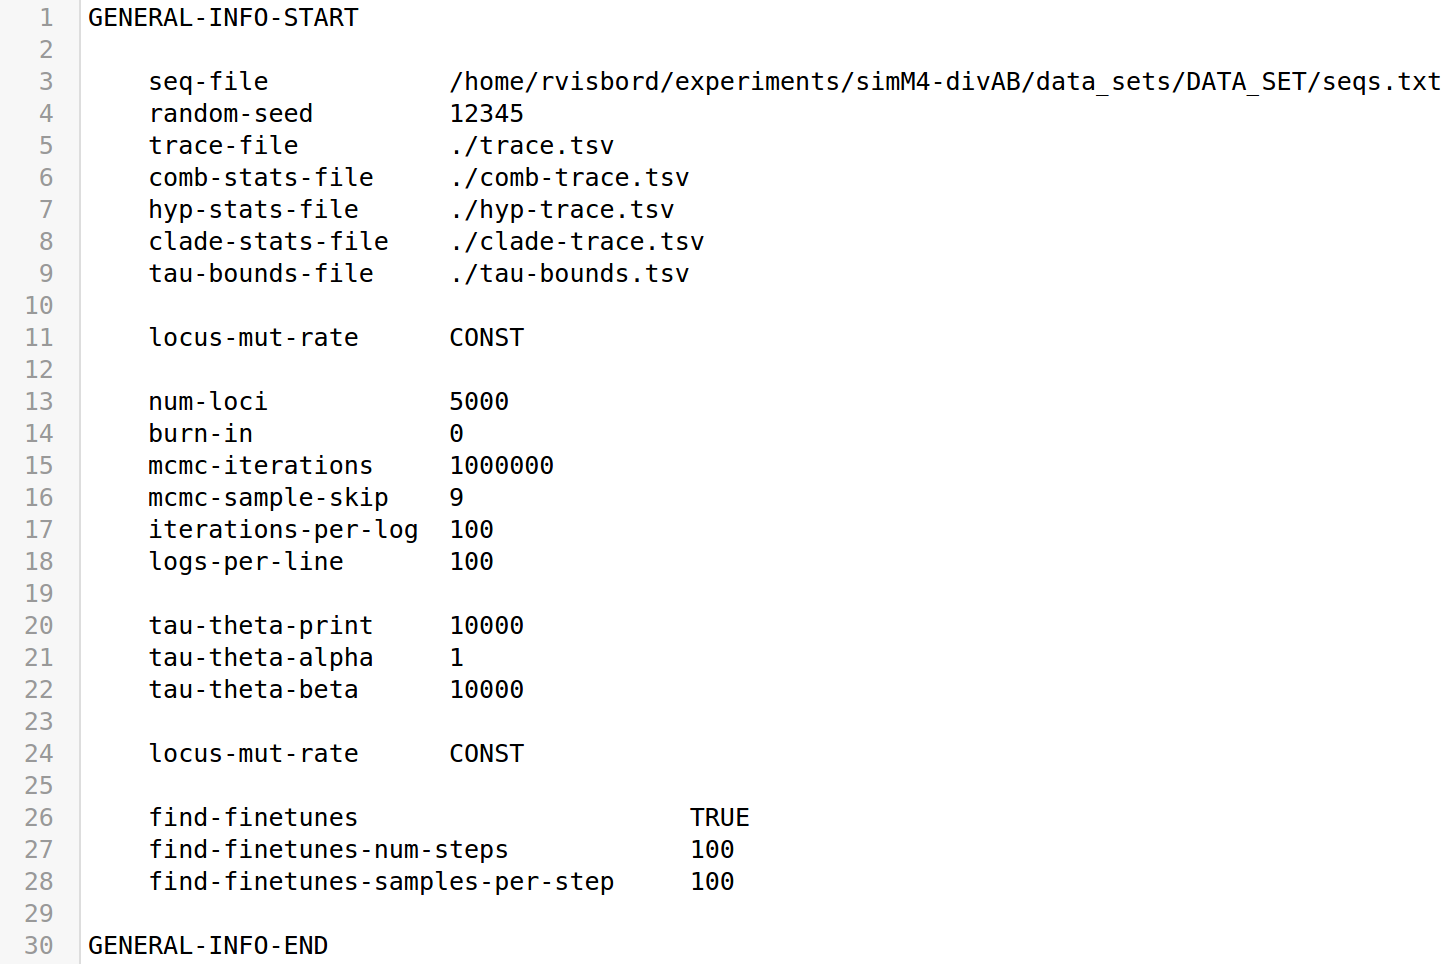
\includegraphics[width=0.8\textwidth]{appendix/general_info}
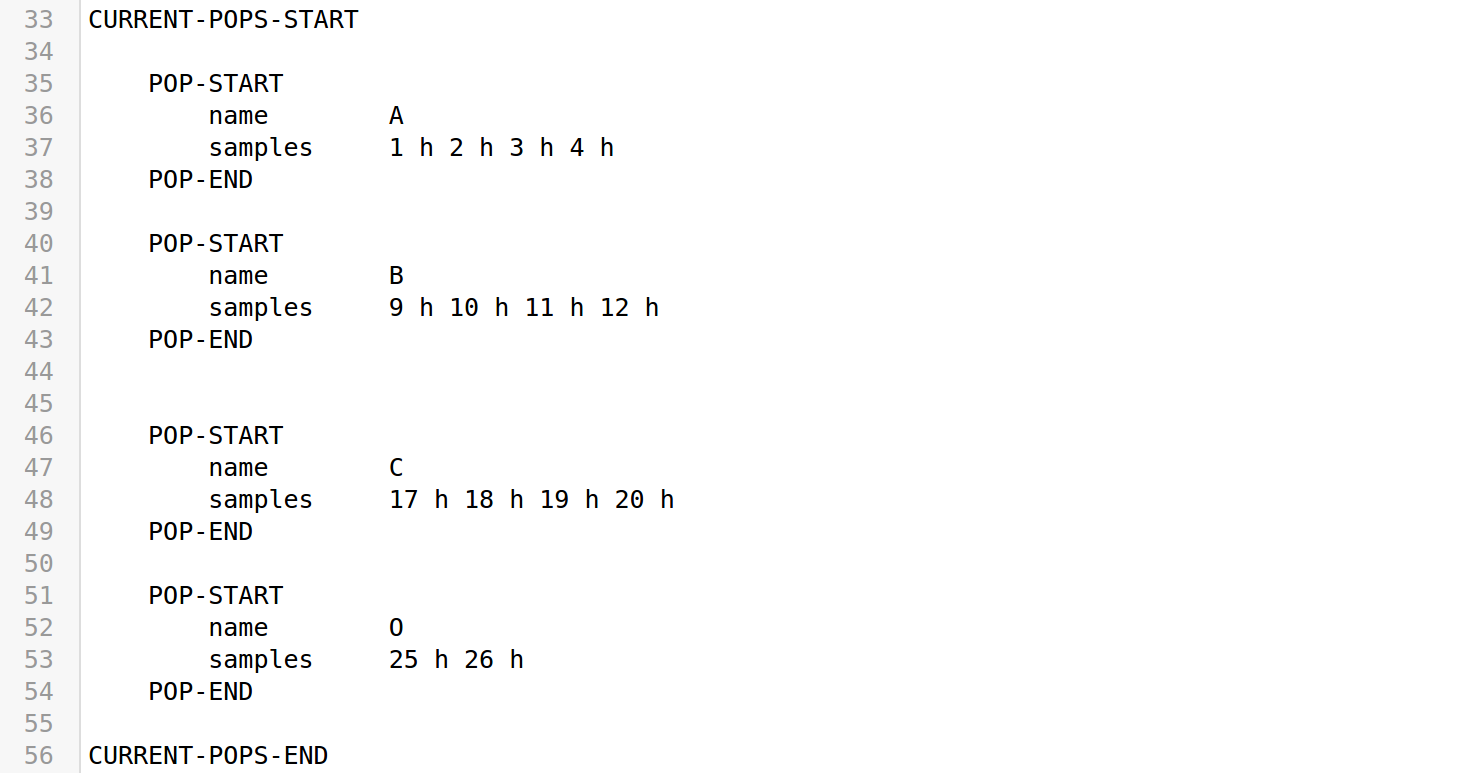
\includegraphics[width=0.8\textwidth]{appendix/current_pops}
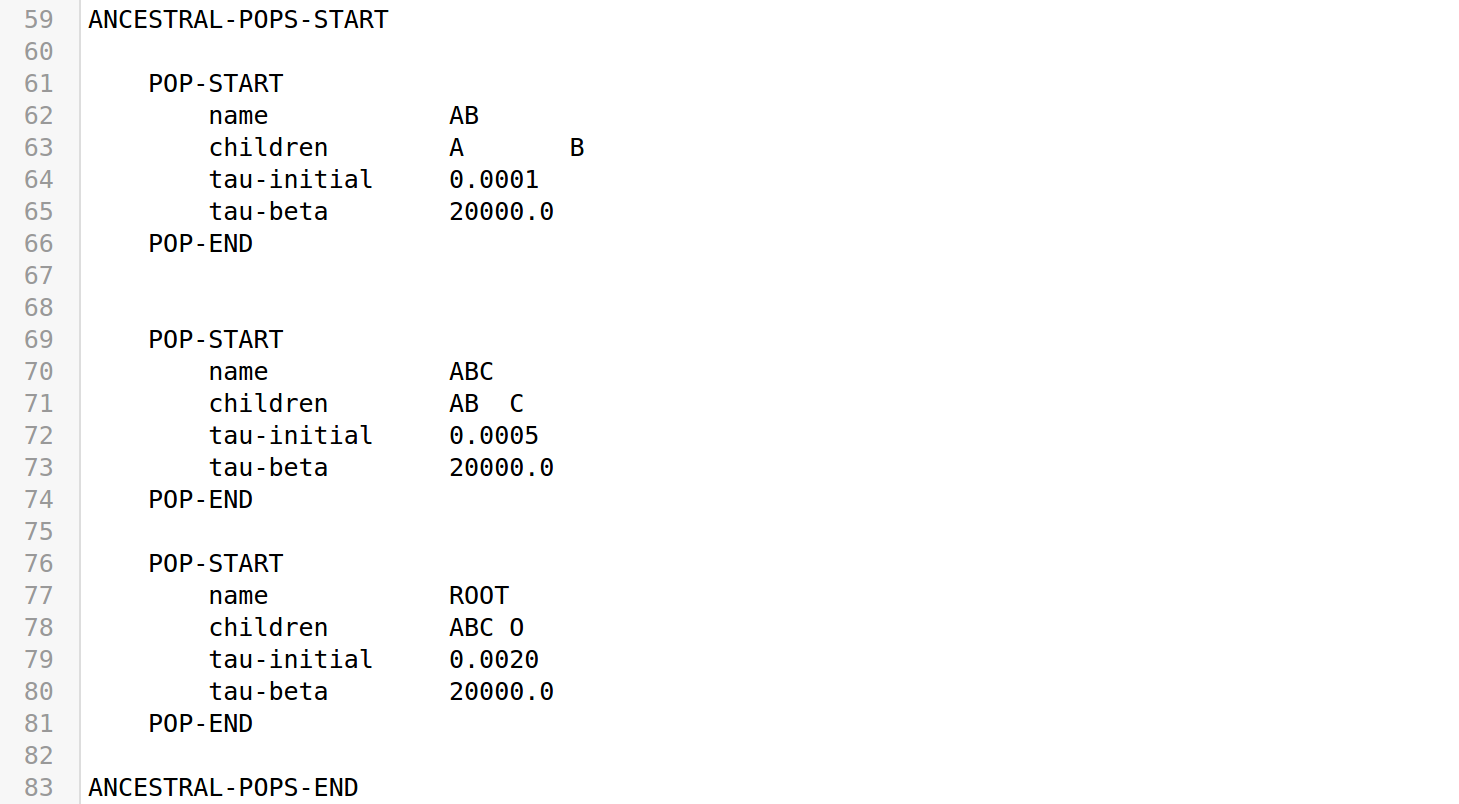
\includegraphics[width=0.8\textwidth]{appendix/ancestral_pops}
\label{fig:sample_McRef_output}
\end{figure}

\noindent\rule{16cm}{0.4pt}

\begin{figure}[H]
\figuretitle{Sample \gp traces of sufficient stats}
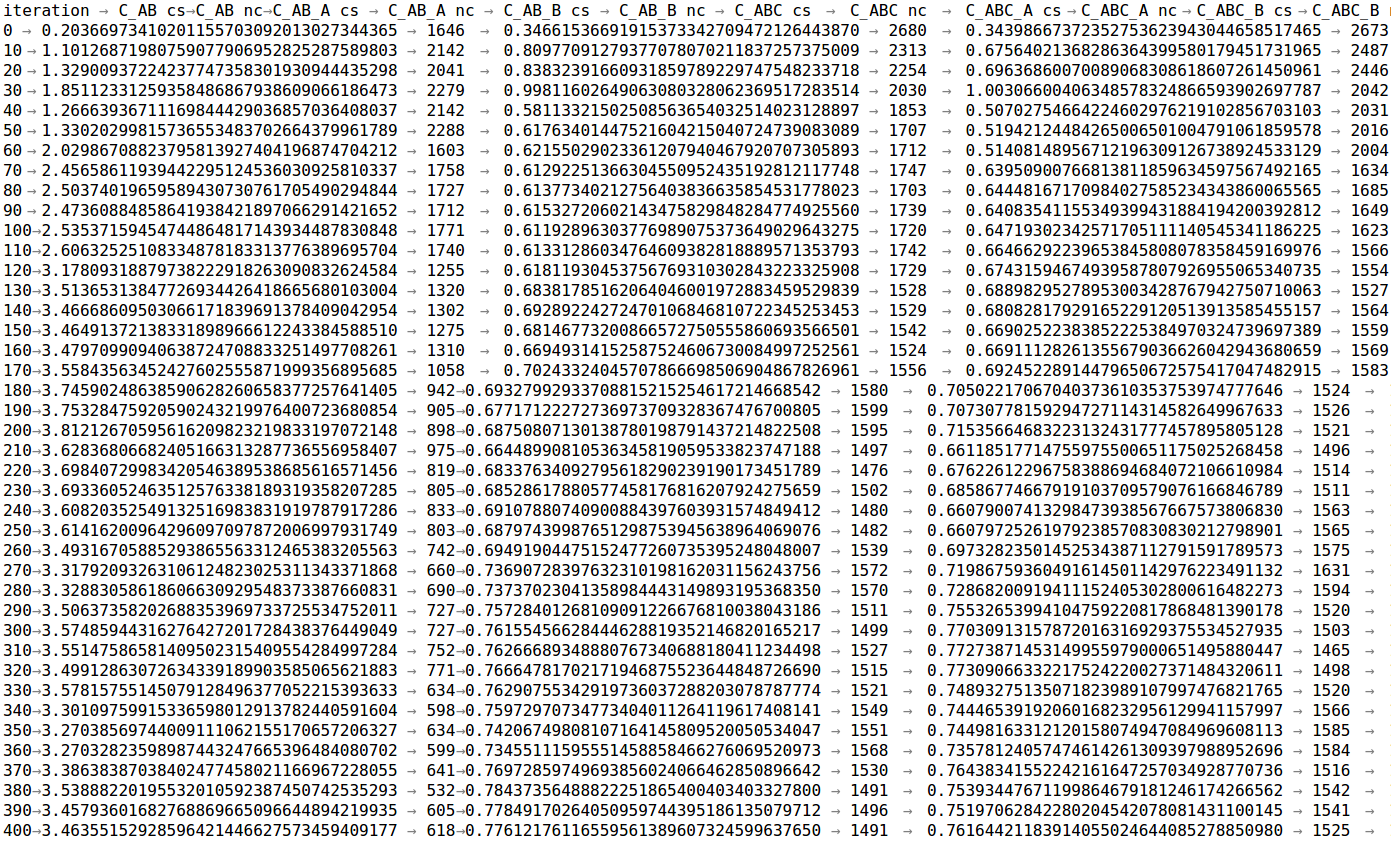
\includegraphics[width=1.0\textwidth]{appendix/sample_gphocs_sufficient_stats_trace}
\label{fig:sample_McRef_output}
\end{figure}

\noindent\rule{16cm}{0.4pt}

\begin{figure}[H]
\figuretitle{Sample McRef \textit{config.ini} for a comb reference model from experiment II}
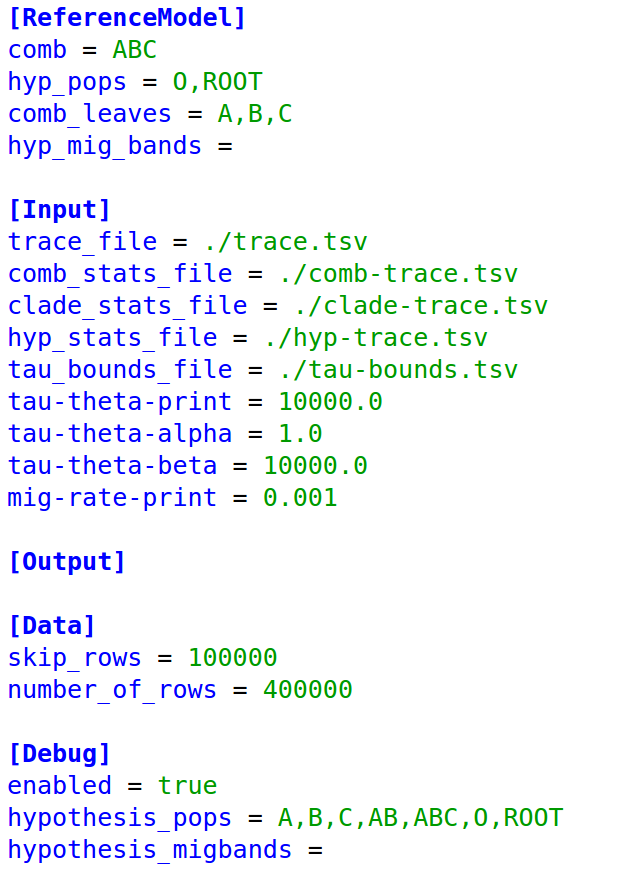
\includegraphics[width=0.5\textwidth]{appendix/sample_McRef_configuration}
\label{fig:sample_McRef_output}
\end{figure}

\noindent\rule{16cm}{0.4pt}

\begin{figure}[H]
\figuretitle{Sample McRef Output from experiment II}
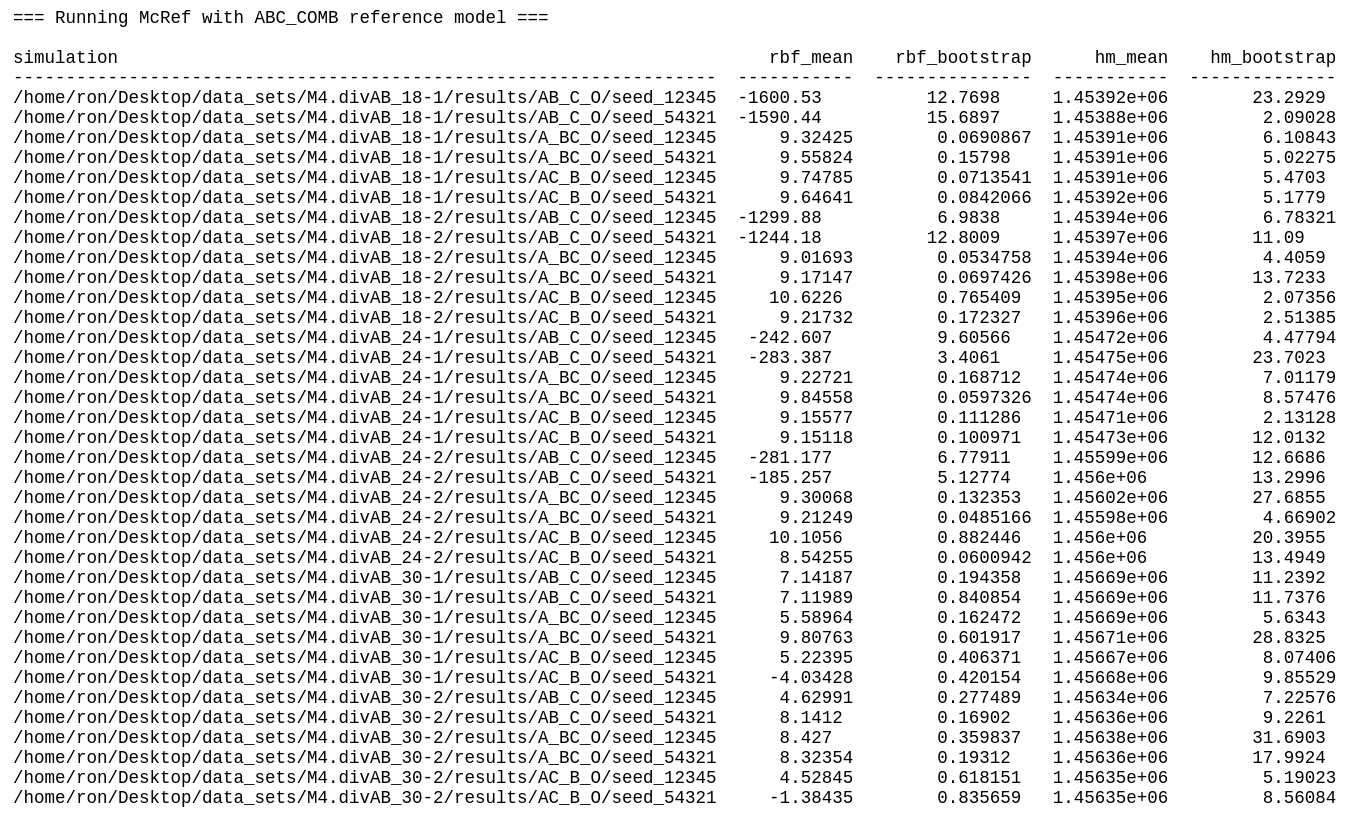
\includegraphics[width=1.0\textwidth]{appendix/sample_McRef_output}
\label{fig:sample_McRef_output}
\end{figure}

\noindent\rule{16cm}{0.4pt}

\begin{figure}[H]
\figuretitle{Sample McRef debug plot of reference population genealogy likelihoods}
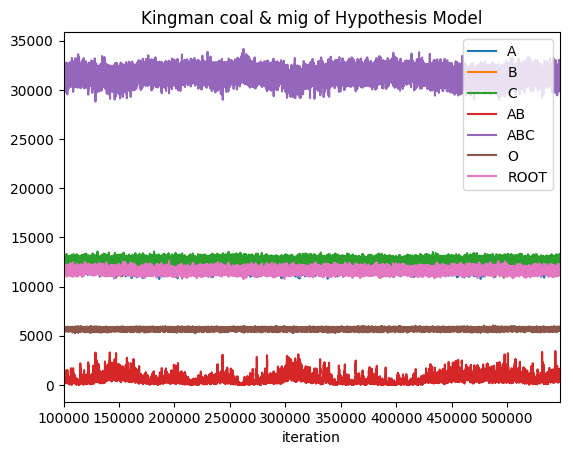
\includegraphics[width=0.9\textwidth]{appendix/hyp_ln_ld_line}
\label{fig:sample_McRef_output}
\end{figure}

\end{document}
